%%%%%%%%%%%%%%%%%%%%%%%%%%%%%%%%%%%%%%%%%%%%%%%%%%%%%%%%%%%%%%%%%%%%%%
% Template for a UBC-compliant dissertation
% At the minimum, you will need to change the information found
% after the "Document meta-data"
%
%!TEX TS-program = pdflatex
%!TEX encoding = UTF-8 Unicode

%% The ubcdiss class provides several options:
%%   gpscopy (aka fogscopy)
%%       set parameters to exactly how GPS specifies
%%         * single-sided
%%         * page-numbering starts from title page
%%         * the lists of figures and tables have each entry prefixed
%%           with 'Figure' or 'Table'
%%       This can be tested by `\ifgpscopy ... \else ... \fi'
%%   10pt, 11pt, 12pt
%%       set default font size
%%   oneside, twoside
%%       whether to format for single-sided or double-sided printing
%%   balanced
%%       when double-sided, ensure page content is centred
%%       rather than slightly offset (the default)
%%   singlespacing, onehalfspacing, doublespacing
%%       set default inter-line text spacing; the ubcdiss class
%%       provides \textspacing to revert to this configured spacing
%%   draft
%%       disable more intensive processing, such as including
%%       graphics, etc.
%%

% For submission to GPS
\documentclass[gpscopy,onehalfspacing,11pt]{ubcdiss}

% For your own copies (looks nicer)
% \documentclass[balanced,twoside,11pt]{ubcdiss}

%%%%%%%%%%%%%%%%%%%%%%%%%%%%%%%%%%%%%%%%%%%%%%%%%%%%%%%%%%%%%%%%%%%%%%
%%%%%%%%%%%%%%%%%%%%%%%%%%%%%%%%%%%%%%%%%%%%%%%%%%%%%%%%%%%%%%%%%%%%%%
%%
%% FONTS:
%% 
%% The defaults below configures Times Roman for the serif font,
%% Helvetica for the sans serif font, and Courier for the
%% typewriter-style font.  Configuring fonts can be time
%% consuming; we recommend skipping to END FONTS!
%% 
%% If you're feeling brave, have lots of time, and wish to use one
%% your platform's native fonts, see the commented out bits below for
%% XeTeX/XeLaTeX.  This is not for the faint at heart. 
%% (And shouldn't you be writing? :-)
%%

%% NFSS font specification (New Font Selection Scheme)
\usepackage{times,mathptmx,courier}
\usepackage[scaled=.92]{helvet}

%% Math or theory people may want to include the handy AMS macros
%\usepackage{amssymb}
%\usepackage{amsmath}
%\usepackage{amsfonts}

%% The pifont package provides access to the elements in the dingbat font.   
%% Use \ding{##} for a particular dingbat (see p7 of psnfss2e.pdf)
%%   Useful:
%%     51,52 different forms of a checkmark
%%     54,55,56 different forms of a cross (saltyre)
%%     172-181 are 1-10 in open circle (serif)
%%     182-191 are 1-10 black circle (serif)
%%     192-201 are 1-10 in open circle (sans serif)
%%     202-211 are 1-10 in black circle (sans serif)
%% \begin{dinglist}{##}\item... or dingautolist (which auto-increments)
%% to create a bullet list with the provided character.
\usepackage{pifont}
\usepackage{graphicx}
\usepackage{textcomp}
\usepackage{xcolor}
\usepackage{amsmath}
\usepackage{amsthm}
\usepackage{ gensymb }
\usepackage{ upgreek }
\usepackage{xspace}
\usepackage{longtable}
\theoremstyle{plain}
\usepackage{array}
\long\def\authornote#1{%
	\leavevmode\unskip\raisebox{-3.5pt}{\rlap{$\scriptstyle\diamond$}}%
	\marginpar{\raggedright\hbadness=10000
		\def\baselinestretch{0.8}\tiny
		\it #1\par}}

\newcommand{\pu}[1]{\authornote{PM: #1}}
\newcommand{\karthik}[1]{\authornote{KP: #1}}
\usepackage{cite}
\usepackage{amsmath,amssymb,amsfonts}
\usepackage[linesnumbered,ruled,vlined]{algorithm2e}
\usepackage{siunitx}
\usepackage{multirow}
\usepackage{blindtext}
\newtheorem{problem}{P}
\newtheorem*{approach*}{Approach}


\newcolumntype{L}[1]{>{\raggedright\let\newline\\\arraybackslash\hspace{0pt}}m{#1}}
\newcolumntype{C}[1]{>{\centering\let\newline\\\arraybackslash\hspace{0pt}}m{#1}}
\newcolumntype{R}[1]{>{\raggedleft\let\newline\\\arraybackslash\hspace{0pt}}m{#1}}
%%%%%%%%%%%%%%%%%%%%%%%%%%%%%%%%%%%%%%%%%%%%%%%%%%%%%%%%%%%%%%%%%%%%%%
%% Configure fonts for XeTeX / XeLaTeX using the fontspec package.
%% Be sure to check out the fontspec documentation.
%\usepackage{fontspec,xltxtra,xunicode}	% required
%\defaultfontfeatures{Mapping=tex-text}	% recommended
%% Minion Pro and Myriad Pro are shipped with some versions of
%% Adobe Reader.  Adobe representatives have commented that these
%% fonts can be used outside of Adobe Reader.
%\setromanfont[Numbers=OldStyle]{Minion Pro}
%\setsansfont[Numbers=OldStyle,Scale=MatchLowercase]{Myriad Pro}
%\setmonofont[Scale=MatchLowercase]{Andale Mono}

%% Other alternatives:
%\setromanfont[Mapping=tex-text]{Adobe Caslon}
%\setsansfont[Scale=MatchLowercase]{Gill Sans}
%\setsansfont[Scale=MatchLowercase,Mapping=tex-text]{Futura}
%\setmonofont[Scale=MatchLowercase]{Andale Mono}
%\newfontfamily{\SYM}[Scale=0.9]{Zapf Dingbats}
%% END FONTS
%%%%%%%%%%%%%%%%%%%%%%%%%%%%%%%%%%%%%%%%%%%%%%%%%%%%%%%%%%%%%%%%%%%%%%
%%%%%%%%%%%%%%%%%%%%%%%%%%%%%%%%%%%%%%%%%%%%%%%%%%%%%%%%%%%%%%%%%%%%%%



%%%%%%%%%%%%%%%%%%%%%%%%%%%%%%%%%%%%%%%%%%%%%%%%%%%%%%%%%%%%%%%%%%%%%%
%%%%%%%%%%%%%%%%%%%%%%%%%%%%%%%%%%%%%%%%%%%%%%%%%%%%%%%%%%%%%%%%%%%%%%
%%
%% Recommended packages
%%
\usepackage{checkend}	% better error messages on left-open environments
\usepackage{graphicx}	% for incorporating external images

%% booktabs: provides some special commands for typesetting tables as used
%% in excellent journals.  Ignore the examples in the Lamport book!
\usepackage{booktabs}

%% listings: useful support for including source code listings, with
%% optional special keyword formatting.  The \lstset{} causes
%% the text to be typeset in a smaller sans serif font, with
%% proportional spacing.
\usepackage{listings}
\lstset{basicstyle=\sffamily\scriptsize,showstringspaces=false,fontadjust}

%% The acronym package provides support for defining acronyms, providing
%% their expansion when first used, and building glossaries.  See the
%% example in glossary.tex and the example usage throughout the example
%% document.
%% NOTE: to use \MakeTextLowercase in the \acsfont command below,
%%   we *must* use the `nohyperlinks' option -- it causes errors with
%%   hyperref otherwise.  See Section 5.2 in the ``LaTeX 2e for Class
%%   and Package Writers Guide'' (clsguide.pdf) for details.
\usepackage[printonlyused,nohyperlinks]{acronym}
%% The ubcdiss.cls loads the `textcase' package which provides commands
%% for upper-casing and lower-casing text.  The following causes
%% the acronym package to typeset acronyms in small-caps
%% as recommended by Bringhurst.
\renewcommand{\acsfont}[1]{{\scshape \MakeTextLowercase{#1}}}

%% color: add support for expressing colour models.  Grey can be used
%% to great effect to emphasize other parts of a graphic or text.
%% For an excellent set of examples, see Tufte's "Visual Display of
%% Quantitative Information" or "Envisioning Information".
\usepackage{color}
\definecolor{greytext}{gray}{0.5}

%% comment: provides a new {comment} environment: all text inside the
%% environment is ignored.
%%   \begin{comment} ignored text ... \end{comment}
\usepackage{comment}

%% The natbib package provides more sophisticated citing commands
%% such as \citeauthor{} to provide the author names of a work,
%% \citet{} to produce an author-and-reference citation,
%% \citep{} to produce a parenthetical citation.
%% We use \citeeg{} to provide examples
\usepackage[numbers,sort&compress]{natbib}
\newcommand{\citeeg}[1]{\citep[e.g.,][]{#1}}

%% The titlesec package provides commands to vary how chapter and
%% section titles are typeset.  The following uses more compact
%% spacings above and below the title.  The titleformat that follow
%% ensure chapter/section titles are set in singlespace.
\usepackage[compact]{titlesec}
\titleformat*{\section}{\singlespacing\raggedright\bfseries\Large}
\titleformat*{\subsection}{\singlespacing\raggedright\bfseries\large}
\titleformat*{\subsubsection}{\singlespacing\raggedright\bfseries}
\titleformat*{\paragraph}{\singlespacing\raggedright\itshape}

%% The caption package provides support for varying how table and
%% figure captions are typeset.
\usepackage[format=hang,indention=-1cm,labelfont={bf},margin=1em]{caption}

%% url: for typesetting URLs and smart(er) hyphenation.
%% \url{http://...} 
\usepackage{url}
\urlstyle{sf}	% typeset urls in sans-serif


%%%%%%%%%%%%%%%%%%%%%%%%%%%%%%%%%%%%%%%%%%%%%%%%%%%%%%%%%%%%%%%%%%%%%%
%%%%%%%%%%%%%%%%%%%%%%%%%%%%%%%%%%%%%%%%%%%%%%%%%%%%%%%%%%%%%%%%%%%%%%
%%
%% Possibly useful packages: you may need to explicitly install
%% these from CTAN if they aren't part of your distribution;
%% teTeX seems to ship with a smaller base than MikTeX and MacTeX.
%%
%\usepackage{pdfpages}	% insert pages from other PDF files
%\usepackage{longtable}	% provide tables spanning multiple pages
%\usepackage{chngpage}	% support changing the page widths on demand
%\usepackage{tabularx}	% an enhanced tabular environment

%% enumitem: support pausing and resuming enumerate environments.
%\usepackage{enumitem}

%% rotating: provides two environments, sidewaystable and sidewaysfigure,
%% for typesetting tables and figures in landscape mode.  
%\usepackage{rotating}

%% subfig: provides for including subfigures within a figure,
%% and includes being able to separately reference the subfigures.
%\usepackage{subfig}

%% ragged2e: provides several new new commands \Centering, \RaggedLeft,
%% \RaggedRight and \justifying and new environments Center, FlushLeft,
%% FlushRight and justify, which set ragged text and are easily
%% configurable to allow hyphenation.
%\usepackage{ragged2e}

%% The ulem package provides a \sout{} for striking out text and
%% \xout for crossing out text.  The normalem and normalbf are
%% necessary as the package messes with the emphasis and bold fonts
%% otherwise.
%\usepackage[normalem,normalbf]{ulem}    % for \sout

%%%%%%%%%%%%%%%%%%%%%%%%%%%%%%%%%%%%%%%%%%%%%%%%%%%%%%%%%%%%%%%%%%%%%%
%% HYPERREF:
%% The hyperref package provides for embedding hyperlinks into your
%% document.  By default the table of contents, references, citations,
%% and footnotes are hyperlinked.
%%
%% Hyperref provides a very handy command for doing cross-references:
%% \autoref{}.  This is similar to \ref{} and \pageref{} except that
%% it automagically puts in the *type* of reference.  For example,
%% referencing a figure's label will put the text `Figure 3.4'.
%% And the text will be hyperlinked to the appropriate place in the
%% document.
%%
%% Generally hyperref should appear after most other packages

%% The following puts hyperlinks in very faint grey boxes.
%% The `pagebackref' causes the references in the bibliography to have
%% back-references to the citing page; `backref' puts the citing section
%% number.  See further below for other examples of using hyperref.
%% 2009/12/09: now use `linktocpage' (Jacek Kisynski): GPS now prefers
%%   that the ToC, LoF, LoT place the hyperlink on the page number,
%%   rather than the entry text.
\usepackage[bookmarks,bookmarksnumbered,%
    allbordercolors={0.8 0.8 0.8},%
    pagebackref,linktocpage%
    ]{hyperref}
%% The following change how the the back-references text is typeset in a
%% bibliography when `backref' or `pagebackref' are used
%%
%% Change \nocitations if you'd like some text shown where there
%% are no citations found (e.g., pulled in with \nocite{xxx})
\newcommand{\nocitations}{\relax}
%%\newcommand{\nocitations}{No citations}
%%
%\renewcommand*{\backref}[1]{}% necessary for backref < 1.33
\renewcommand*{\backrefsep}{,~}%
\renewcommand*{\backreftwosep}{,~}% ', and~'
\renewcommand*{\backreflastsep}{,~}% ' and~'
\renewcommand*{\backrefalt}[4]{%
\textcolor{greytext}{\ifcase #1%
\nocitations%
\or
\(\rightarrow\) page #2%
\else
\(\rightarrow\) pages #2%
\fi}}


%% The following uses most defaults, which causes hyperlinks to be
%% surrounded by colourful boxes; the colours are only visible in
%% PDFs and don't show up when printed:
%\usepackage[bookmarks,bookmarksnumbered]{hyperref}

%% The following disables the colourful boxes around hyperlinks.
%\usepackage[bookmarks,bookmarksnumbered,pdfborder={0 0 0}]{hyperref}

%% The following disables all hyperlinking, but still enabled use of
%% \autoref{}
%\usepackage[draft]{hyperref}

%% The following commands causes chapter and section references to
%% uppercase the part name.
\renewcommand{\chapterautorefname}{Chapter}
\renewcommand{\sectionautorefname}{Section}
\renewcommand{\subsectionautorefname}{Section}
\renewcommand{\subsubsectionautorefname}{Section}

%% If you have long page numbers (e.g., roman numbers in the 
%% preliminary pages for page 28 = xxviii), you might need to
%% uncomment the following and tweak the \@pnumwidth length
%% (default: 1.55em).  See the tocloft documentation at
%% http://www.ctan.org/tex-archive/macros/latex/contrib/tocloft/
% \makeatletter
% \renewcommand{\@pnumwidth}{3em}
% \makeatother

%%%%%%%%%%%%%%%%%%%%%%%%%%%%%%%%%%%%%%%%%%%%%%%%%%%%%%%%%%%%%%%%%%%%%%
%%%%%%%%%%%%%%%%%%%%%%%%%%%%%%%%%%%%%%%%%%%%%%%%%%%%%%%%%%%%%%%%%%%%%%
%%
%% Some special settings that controls how text is typeset
%%
% \raggedbottom		% pages don't have to line up nicely on the last line
% \sloppy		% be a bit more relaxed in inter-word spacing
% \clubpenalty=10000	% try harder to avoid orphans
% \widowpenalty=10000	% try harder to avoid widows
% \tolerance=1000

%% And include some of our own useful macros
% This file provides examples of some useful macros for typesetting
% dissertations.  None of the macros defined here are necessary beyond
% for the template documentation, so feel free to change, remove, and add
% your own definitions.
%
% We recommend that you define macros to separate the semantics
% of the things you write from how they are presented.  For example,
% you'll see definitions below for a macro \file{}: by using
% \file{} consistently in the text, we can change how filenames
% are typeset simply by changing the definition of \file{} in
% this file.
% 
%% The following is a directive for TeXShop to indicate the main file
%%!TEX root = diss.tex
\newcommand{\tool}{{\em ReLUSyn }}
\newcommand{\attack}{{\em ripple FDI attack }}
\newcommand{\NA}{\textsc{n/a}}	% for "not applicable"
\newcommand{\eg}{e.g.,\ }	% proper form of examples (\eg a, b, c)
\newcommand{\ie}{i.e.,\ }	% proper form for that is (\ie a, b, c)
\newcommand{\etal}{\emph{et al}}

% Some useful macros for typesetting terms.
\newcommand{\file}[1]{\texttt{#1}}
\newcommand{\class}[1]{\texttt{#1}}
\newcommand{\latexpackage}[1]{\href{http://www.ctan.org/macros/latex/contrib/#1}{\texttt{#1}}}
\newcommand{\latexmiscpackage}[1]{\href{http://www.ctan.org/macros/latex/contrib/misc/#1.sty}{\texttt{#1}}}
\newcommand{\env}[1]{\texttt{#1}}
\newcommand{\BibTeX}{Bib\TeX}

% Define a command \doi{} to typeset a digital object identifier (DOI).
% Note: if the following definition raise an error, then you likely
% have an ancient version of url.sty.  Either find a more recent version
% (3.1 or later work fine) and simply copy it into this directory,  or
% comment out the following two lines and uncomment the third.
\DeclareUrlCommand\DOI{}
\newcommand{\doi}[1]{\href{http://dx.doi.org/#1}{\DOI{doi:#1}}}
%\newcommand{\doi}[1]{\href{http://dx.doi.org/#1}{doi:#1}}

% Useful macro to reference an online document with a hyperlink
% as well with the URL explicitly listed in a footnote
% #1: the URL
% #2: the anchoring text
\newcommand{\webref}[2]{\href{#1}{#2}\footnote{\url{#1}}}

% epigraph is a nice environment for typesetting quotations
\makeatletter
\newenvironment{epigraph}{%
	\begin{flushright}
	\begin{minipage}{\columnwidth-0.75in}
	\begin{flushright}
	\@ifundefined{singlespacing}{}{\singlespacing}%
    }{
	\end{flushright}
	\end{minipage}
	\end{flushright}}
\makeatother

% \FIXME{} is a useful macro for noting things needing to be changed.
% The following definition will also output a warning to the console
\newcommand{\FIXME}[1]{\typeout{**FIXME** #1}\textbf{[FIXME: #1]}}

% END


%%%%%%%%%%%%%%%%%%%%%%%%%%%%%%%%%%%%%%%%%%%%%%%%%%%%%%%%%%%%%%%%%%%%%%
%%%%%%%%%%%%%%%%%%%%%%%%%%%%%%%%%%%%%%%%%%%%%%%%%%%%%%%%%%%%%%%%%%%%%%
%%
%% Document meta-data: be sure to also change the \hypersetup information
%%

\title{Security analysis of Deep Neural Network Based Cyber-Physical Systems.}
%\subtitle{If you want a subtitle}

\author{Aarti Kashyap}
\previousdegree{B. Technology, College of Engineering Pune, 2018}


% What is this dissertation for?
\degreetitle{Master of Applied Science}

\institution{The University of British Columbia}
\campus{Vancouver}

\faculty{The Faculty of graduate and postdoctoral studies}
\department{Computer Engineering}
\submissionmonth{}
\submissionyear{2020}

% details of your examining committee
\examiningcommittee{Karthik Pattabiraman, Electrical and Computer Engineering}{Supervisor}
\examiningcommittee{Margo Seltzer, Computer Science}{Committee member}
\examiningcommittee{Sathish Gopalakrishnan, Electrical and Computer Engineering}{Chair}
\iffalse
\examiningcommittee{Mary Maker, Materials Engineering}%
    {Supervisory Committee Member}
\examiningcommittee{Nebulous Name, Department}{Supervisory Committee Member}
\examiningcommittee{Magnus Monolith, Other Department}{Additional Examiner}

% details of your supervisory committee
\supervisorycommittee{Karthik Pattabiraman, Electrical and Computer Engineering}%
    {Supervisory Committee Member}
\supervisorycommittee{Adeline Long, \textsc{CEO} of Aerial Machine
    Transportation, Inc.}{Supervisory Committee Member}
\fi
%% hyperref package provides support for embedding meta-data in .PDF
%% files
\hypersetup{
  pdftitle={Change this title!  (DRAFT: \today)},
  pdfauthor={Johnny Canuck},
  pdfkeywords={Your keywords here}
}

%%%%%%%%%%%%%%%%%%%%%%%%%%%%%%%%%%%%%%%%%%%%%%%%%%%%%%%%%%%%%%%%%%%%%%
%%%%%%%%%%%%%%%%%%%%%%%%%%%%%%%%%%%%%%%%%%%%%%%%%%%%%%%%%%%%%%%%%%%%%%
%% 
%% The document content
%%

%% LaTeX's \includeonly commands causes any uses of \include{} to only
%% include files that are in the list.  This is helpful to produce
%% subsets of your thesis (e.g., for committee members who want to see
%% the dissertation chapter by chapter).  It also saves time by 
%% avoiding reprocessing the entire file.
%\includeonly{intro,conclusions}
%\includeonly{discussion}

\begin{document}

%%%%%%%%%%%%%%%%%%%%%%%%%%%%%%%%%%%%%%%%%%%%%%%%%%
%% From Thesis Components: Tradtional Thesis
%% <http://www.grad.ubc.ca/current-students/dissertation-thesis-preparation/order-components>

% Preliminary Pages (numbered in lower case Roman numerals)
%    1. Title page (mandatory)
\maketitle

%    2. Committee page (mandatory): lists supervisory committee and,
%    if applicable, the examining committee
\makecommitteepage

%    3. Abstract (mandatory - maximum 350 words)
%% The following is a directive for TeXShop to indicate the main file
%%!TEX root = diss.tex

\chapter{Abstract}

\ac{CPS} are deployed in many mission-critical applications such as medical devices (e.g., an \ac{APS}), autonomous vehicular systems (e.g., self-driving cars, unmanned aerial vehicles) and aircraft control management systems (e.g.,  \ac{HCAS} and \ac{ACAS-Xu}). 
Ensuring correctness is becoming more difficult as these systems adopt new technology, such as \ac{DNN}, to control these systems. 
\ac{DNN} are black box algorithms whose inner workings are complex and difficult to discern.
As such, understanding their vulnerabilities is also complex and difficult. 

We identify a new vulnerability in these systems and demonstrate how to synthesize a new category of attacks \ac{RFDIA} in them by perturbing specific inputs, by minimal amounts to stealthily change the \ac{DNN}'s output. 
 These  perturbations propagate as ripples through multiple \ac{DNN} layers and can lead to corruptions that can be fatal. 
We demonstrate that it is possible  to construct such attacks efficiently by identifying the \ac{DNN}'s critical inputs. 
The critical inputs are those that  affect the final outputs the most on being perturbed. 
Understanding this new class of attacks sets the stage for developing methods to mitigate vulnerabilities. 

Our attack synthesis technique is based on modeling the attack as an optimization problem using \ac{MILP}.
We define an abstraction for \ac{DNN}-based \ac{CPS} that allows us to automatically: 1) identify the critical inputs, and 2) find the smallest perturbations that produce output changes. 
We demonstrate our technique on three practical \ac{CPS} with two mission-critical applications in increasing order of complexity: Medical systems (\ac{APS}) and aircraft control management systems (\ac{HCAS} and \ac{ACAS-Xu}). 
Our key observations for scaling our technique to complex systems such as \ac{ACAS-Xu} were to define: 1) appropriate intervals for their inputs and the outputs, and 2) attack specific objective (cost) functions in the abstraction.  
 



% Consider placing version information if you circulate multiple drafts
%\vfill
%\begin{center}
%\begin{sf}
%\fbox{Revision: \today}
%\end{sf}
%\end{center}

\cleardoublepage

%    4. Lay Summary (Effective May 2017, mandatory - maximum 150 words)
%% The following is a directive for TeXShop to indicate the main file
%%!TEX root = diss.tex

%% https://www.grad.ubc.ca/current-students/dissertation-thesis-preparation/preliminary-pages
%% 
%% LAY SUMMARY Effective May 2017, all theses and dissertations must
%% include a lay summary.  The lay or public summary explains the key
%% goals and contributions of the research/scholarly work in terms that
%% can be understood by the general public. It must not exceed 150
%% words in length.

\chapter{Lay Summary}

Cyber-physical systems (CPS) are systems that perform computations by continuous interactions with the physical environment and perform actions in the physical environment based on the computations. 
\ac{CPS} are deployed in many mission-critical applications such as medical devices, autonomous vehicular systems (e.g., self-driving cars, unmanned aerial vehicles), and aircraft control management systems. 
This mission-critical aspect of \ac{CPS} suggests that ensuring their correct functioning, and complying with all safety specifications is of paramount importance. 
Ensuring correctness is becoming more difficult as these systems adopt new technology, such as Deep Neural Networks (DNN), to control them. 
\ac{DNN} are black box algorithms whose inner workings are complex and difficult to discern.
As such, understanding their vulnerabilities is also difficult. 

This exposes new vulnerabilities by introducing a  technique to produce attacks that can alter the behavior of the system in unexpected ways. 
Understanding this new class of attacks is the first step towards developing methods to mitigate these vulnerabilities. 



 


%Basically three things are being done here
%1- new category of attacks
%2- formalised them
%3- showed them on three different systems


\cleardoublepage

%    5. Preface
%% The following is a directive for TeXShop to indicate the main file
%%!TEX root = diss.tex

\chapter{Preface}

I was responsible for shaping the key idea, leading the project, designing the experiments, analyzing the results, and writing the work.
Prof. Karthik Pattabiraman was responsible for overseeing the project and discussions.
Prof. Margo Seltzer helped in writing and editing the drafts and analyzing the results. 
Mubashir Iqbal contributed with his prior knowledge and expertise in the area and helped with the experiments.

\cleardoublepage

%    6. Table of contents (mandatory - list all items in the preliminary pages
%    starting with the abstract, followed by chapter headings and
%    subheadings, bibliographies and appendices)
\tableofcontents
\cleardoublepage	% required by tocloft package

%    7. List of tables (mandatory if thesis has tables)
\listoftables
\cleardoublepage	% required by tocloft package

%    8. List of figures (mandatory if thesis has figures)
\listoffigures
\cleardoublepage	% required by tocloft package

%    9. List of illustrations (mandatory if thesis has illustrations)
%   10. Lists of symbols, abbreviations or other (optional)

%   11. Glossary (optional)
%% The following is a directive for TeXShop to indicate the main file
%%!TEX root = diss.tex

\chapter{Glossary}

%This glossary uses the handy \latexpackage{acroynym} package to automatically
%maintain the glossary.  It uses the package's \texttt{printonlyused}
%option to include only those acronyms explicitly referenced in the
%\LaTeX\ source.

% use \acrodef to define an acronym, but no listing
\acrodef{UI}{user interface}
\acrodef{UBC}{University of British Columbia}

% The acronym environment will typeset only those acronyms that were
% *actually used* in the course of the document
\begin{acronym}[ANOVA]
	\acro{ANOVA}[ANOVA]{Analysis of Variance\acroextra{, a set of
			statistical techniques to identify sources of variability between groups}}
	\acro{API}{application programming interface}
	\acro{CTAN}{\acroextra{The }Common \TeX\ Archive Network}
	\acro{DOI}{Document Object Identifier\acroextra{ (see
			\url{http://doi.org})}}
	\acro{GPS}[GPS]{Graduate and Postdoctoral Studies}
	\acro{PDF}{Portable Document Format}
	\acro{RCS}[RCS]{Revision control system\acroextra{, a software
			tool for tracking changes to a set of files}}
	\acro{TLX}[TLX]{Task Load Index\acroextra{, an instrument for gauging
			the subjective mental workload experienced by a human in performing
			a task}}
	\acro{UML}{Unified Modelling Language\acroextra{, a visual language
			for modelling the structure of software artefacts}}
	\acro{URL}{Unique Resource Locator\acroextra{, used to describe a
			means for obtaining some resource on the world wide web}}
	\acro{W3C}[W3C]{\acroextra{the }World Wide Web Consortium\acroextra{,
			the standards body for web technologies}}
	\acro{XML}{Extensible Markup Language}
	
		\acro{ACAS-Xu}{Collision Avoidance System-Xu}
		\acro{APS}{Artifical Pancreas System}
				\acro{AV}{Autonomous Vehicles}
					\acro{CA}{Collision Avoidance}
		\acro{CPS}{Cyber Physical Systems}
			\acro{CGM}{Continuous Glucose Monitor}
	\acro{DNN}{Deep Neural Network}
\acro{FDIA}{False Data Injection Attacks}
	\acro{ReLUSyn}{ReLU Synthesizer}
		\acro{HCAS}{Horizontal Collision Avoidance System}
		\acro{LP}{Linear Programs}
			\acro{MILP}{Mixed Integer Linear Programming}
		\acro{MIP}{Mixed Integer Programs}
		
		
		
		\acro{ML}{Machine Learning}
			\acro{NN}{Neural Network}
	\acro{RFDIA}{Ripple False Data Injection Attacks}


	\acro{RPi}{Raspberry Pi}



		\acro{ReLU}{Rectified Linear Unit}
		\acro{SMT}{Satisfiability Modulo Theories}
\end{acronym}

% You can also use \newacro{}{} to only define acronyms
% but without explictly creating a glossary
% 
% \newacro{ANOVA}[ANOVA]{Analysis of Variance\acroextra{, a set of
%   statistical techniques to identify sources of variability between groups.}}
% \newacro{API}[API]{application programming interface}
% \newacro{GOMS}[GOMS]{Goals, Operators, Methods, and Selection\acroextra{,
%   a framework for usability analysis.}}
% \newacro{TLX}[TLX]{Task Load Index\acroextra{, an instrument for gauging
%   the subjective mental workload experienced by a human in performing
%   a task.}}
% \newacro{UI}[UI]{user interface}
% \newacro{UML}[UML]{Unified Modelling Language}
% \newacro{W3C}[W3C]{World Wide Web Consortium}
% \newacro{XML}[XML]{Extensible Markup Language}
	% always input, since other macros may rely on it

\textspacing		% begin one-half or double spacing

%   12. Acknowledgements (optional)
%% The following is a directive for TeXShop to indicate the main file
%%!TEX root = diss.tex

\chapter{Acknowledgments}

I would like to thank the following:
My advisor, Karthik Pattabiraman, for allowing me to pursue my ideas and explore during my masters which was my original goal. I've learned a lot from him. 

Margo Seltzer for being a constant source of inspiration that helped me pursue my ideas fearlessly and enjoy research during my masters. Without her, this thesis would not have been possible. 

Syed Mubashir Iqbal for collaborating on this work and teaching me a bunch of stuff; working with Mubashir was one of the most fun experiences of my master's thesis because of the infinite all-nighters we pulled off to finish the experiments in ICICS 348. 

Mark Greenstreet, Alan Hu, Hassan Halawa and Puneet Mehrotra for patiently listening to my half-baked ideas in the initial stages of the work that eventually lead me to find my path. 

William Bowman for introducing me to the world of abstractions that helped me understand my work a little better.  

Members of the computer systems reading group and static analysis reading group for interesting discussions that might have directly or indirectly influenced my thinking. 

The multiple 'travel granting committees' from conferences that allowed me to
travel all around the world and have many interesting discussions with researchers which might have significantly influenced my thinking. 

Members of Dependable Systems and Systopia (formerly NSS) Lab for multiple fun hangouts. 

The library staff at UBC for always ordering the books I've asked for as soon as possible.

All my friends (y' all know who you are) for being there; listening to my constant bicker about life despite being in different timezones.   

Tom Lee Music store for letting me use their jam room for hours and hours every week since 2018. Surviving the journey without music would be impossible. 

Akshay Gopalakrishnan for ... everything. 

My ma and sister for being ok (or may be pretending to be ok) with my new life plan every other week, thus never holding me back. 






%   13. Dedication (optional)

% Body of Thesis (not all sections may apply)
\mainmatter

\acresetall	% reset all acronyms used so far

%    1. Introduction
%%% The following is a directive for TeXShop to indicate the main file
%%!TEX root = diss.tex
\begin{comment}


\chapter{Introduction}
\label{ch:Introduction}

\begin{epigraph}
    \emph{If I have seen farther it is by standing on the shoulders of
    Giants.} ---~Sir Isaac Newton (1855)
\end{epigraph}

This document provides a quick set of instructions for using the
\class{ubcdiss} class to write a dissertation in \LaTeX. 
Unfortunately this document cannot provide an introduction to using
\LaTeX.  The classic reference for learning \LaTeX\ is
\citeauthor{lamport-1994-ladps}'s
book~\cite{lamport-1994-ladps}.  There are also many freely-available
tutorials online;
\webref{http://www.andy-roberts.net/misc/latex/}{Andy Roberts' online
    \LaTeX\ tutorials}
seems to be excellent.
The source code for this docment, however, is intended to serve as
an example for creating a \LaTeX\ version of your dissertation.

We start by discussing organizational issues, such as splitting
your dissertation into multiple files, in
\autoref{sec:SuggestedThesisOrganization}.
We then cover the ease of managing cross-references in \LaTeX\ in
\autoref{sec:CrossReferences}.
We cover managing and using bibliographies with \BibTeX\ in
\autoref{sec:BibTeX}. 
We briefly describe typesetting attractive tables in
\autoref{sec:TypesettingTables}.
We briefly describe including external figures in
\autoref{sec:Graphics}, and using special characters and symbols
in \autoref{sec:SpecialSymbols}.
As it is often useful to track different versions of your dissertation,
we discuss revision control further in
\autoref{sec:DissertationRevisionControl}. 
We conclude with pointers to additional sources of information in
\autoref{sec:Conclusions}.

%%%%%%%%%%%%%%%%%%%%%%%%%%%%%%%%%%%%%%%%%%%%%%%%%%%%%%%%%%%%%%%%%%%%%%
\section{Suggested Thesis Organization}
\label{sec:SuggestedThesisOrganization}

The \acs{UBC} \acf{GPS} specifies a particular arrangement of the
components forming a thesis.\footnote{See
    \url{http://www.grad.ubc.ca/current-students/dissertation-thesis-preparation/order-components}}
This template reflects that arrangement.

In terms of writing your thesis, the recommended best practice for
organizing large documents in \LaTeX\ is to place each chapter in
a separate file.  These chapters are then included from the main
file through the use of \verb+\include{file}+.  A thesis might
be described as six files such as \file{intro.tex},
\file{relwork.tex}, \file{model.tex}, \file{eval.tex},
\file{discuss.tex}, and \file{concl.tex}.

We also encourage you to use macros for separating how something
will be typeset (\eg bold, or italics) from the meaning of that
something. 
For example, if you look at \file{intro.tex}, you will see repeated
uses of a macro \verb+\file{}+ to indicate file names.
The \verb+\file{}+ macro is defined in the file \file{macros.tex}.
The consistent use of \verb+\file{}+ throughout the text not only
indicates that the argument to the macro represents a file (providing
meaning or semantics), but also allows easily changing how
file names are typeset simply by changing the definition of the
\verb+\file{}+ macro.
\file{macros.tex} contains other useful macros for properly typesetting
things like the proper uses of the latinate \emph{exempli grati\={a}}
and \emph{id est} (\ie \verb+\eg+ and \verb+\ie+), 
web references with a footnoted \acs{URL} (\verb+\webref{url}{text}+),
as well as definitions specific to this documentation
(\verb+\latexpackage{}+).

%%%%%%%%%%%%%%%%%%%%%%%%%%%%%%%%%%%%%%%%%%%%%%%%%%%%%%%%%%%%%%%%%%%%%%
\section{Making Cross-References}
\label{sec:CrossReferences}

\LaTeX\ make managing cross-references easy, and the \latexpackage{hyperref}
package's\ \verb+\autoref{}+ command\footnote{%
    The \latexpackage{hyperref} package is included by default in this
    template.}
makes it easier still. 

A thing to be cross-referenced, such as a section, figure, or equation,
is \emph{labelled} using a unique, user-provided identifier, defined
using the \verb+\label{}+ command.  
The thing is referenced elsewhere using the \verb+\autoref{}+ command.
For example, this section was defined using:
\begin{lstlisting}
    \section{Making Cross-References}
    \label{sec:CrossReferences}
\end{lstlisting}
References to this section are made as follows:
\begin{lstlisting}
    We then cover the ease of managing cross-references in \LaTeX\
    in \autoref{sec:CrossReferences}.
\end{lstlisting}
\verb+\autoref{}+ takes care of determining the \emph{type} of the 
thing being referenced, so the example above is rendered as
\begin{quote}
    We then cover the ease of managing cross-references in \LaTeX\
    in \autoref{sec:CrossReferences}.
\end{quote}

The label is any simple sequence of characters, numbers, digits,
and some punctuation marks such as ``:'' and ``--''; there should
be no spaces.  Try to use a consistent key format: this simplifies
remembering how to make references.  This document uses a prefix
to indicate the type of the thing being referenced, such as \texttt{sec}
for sections, \texttt{fig} for figures, \texttt{tbl} for tables,
and \texttt{eqn} for equations.

For details on defining the text used to describe the type
of \emph{thing}, search \file{diss.tex} and the \latexpackage{hyperref}
documentation for \texttt{autorefname}.


%%%%%%%%%%%%%%%%%%%%%%%%%%%%%%%%%%%%%%%%%%%%%%%%%%%%%%%%%%%%%%%%%%%%%%
\section{Managing Bibliographies with \BibTeX}
\label{sec:BibTeX}

One of the primary benefits of using \LaTeX\ is its companion program,
\BibTeX, for managing bibliographies and citations.  Managing
bibliographies has three parts: (i) describing references,
(ii)~citing references, and (iii)~formatting cited references.

\subsection{Describing References}

\BibTeX\ defines a standard format for recording details about a
reference.  These references are recorded in a file with a
\file{.bib} extension.  \BibTeX\ supports a broad range of
references, such as books, articles, items in a conference proceedings,
chapters, technical reports, manuals, dissertations, and unpublished
manuscripts. 
A reference may include attributes such as the authors,
the title, the page numbers, the \ac{DOI}, or a \ac{URL}.  A reference
can also be augmented with personal attributes, such as a rating,
notes, or keywords.

Each reference must be described by a unique \emph{key}.\footnote{%
    Note that the citation keys are different from the reference
    identifiers as described in \autoref{sec:CrossReferences}.}
A key is a simple sequence of characters, numbers, digits, and some
punctuation marks such as ``:'' and ``--''; there should be no spaces. 
A consistent key format simiplifies remembering how to make references. 
For example:
\begin{quote}
   \fbox{\emph{last-name}}\texttt{-}\fbox{\emph{year}}\texttt{-}\fbox{\emph{contracted-title}}
\end{quote}
where \emph{last-name} represents the last name for the first author,
and \emph{contracted-title} is some meaningful contraction of the
title.  Then \citeauthor{kiczales-1997-aop}'s seminal article on
aspect-oriented programming~\cite{kiczales-1997-aop} (published in
\citeyear{kiczales-1997-aop}) might be given the key
\texttt{kiczales-1997-aop}.

An example of a \BibTeX\ \file{.bib} file is included as
\file{biblio.bib}.  A description of the format a \file{.bib}
file is beyond the scope of this document.  We instead encourage
you to use one of the several reference managers that support the
\BibTeX\ format such as
\webref{http://jabref.sourceforge.net}{JabRef} (multiple platforms) or
\webref{http://bibdesk.sourceforge.net}{BibDesk} (MacOS\,X only). 
These front ends are similar to reference manages such as
EndNote or RefWorks.


\subsection{Citing References}

Having described some references, we then need to cite them.  We
do this using a form of the \verb+\cite+ command.  For example:
\begin{lstlisting}
    \citet{kiczales-1997-aop} present examples of crosscutting 
    from programs written in several languages.
\end{lstlisting}
When processed, the \verb+\citet+ will cause the paper's authors
and a standardized reference to the paper to be inserted in the
document, and will also include a formatted citation for the paper
in the bibliography.  For example:
\begin{quote}
    \citet{kiczales-1997-aop} present examples of crosscutting 
    from programs written in several languages.
\end{quote}
There are several forms of the \verb+\cite+ command (provided
by the \latexpackage{natbib} package), as demonstrated in
\autoref{tbl:natbib:cite}.
Note that the form of the citation (numeric or author-year) depends
on the bibliography style (described in the next section).
The \verb+\citet+ variant is used when the author names form
an object in the sentence, whereas the \verb+\citep+ variant
is used for parenthetic references, more like an end-note.
Use \verb+\nocite+ to include a citation in the bibliography
but without an actual reference.
\nocite{rowling-1997-hpps}
\begin{table}
\caption{Available \texttt{cite} variants; the exact citation style
    depends on whether the bibliography style is numeric or author-year.}
\label{tbl:natbib:cite}
\centering
\begin{tabular}{lp{3.25in}}\toprule
Variant & Result \\
\midrule
% We cheat here to simulate the cite/citep/citet for APA-like styles
\verb+\cite+ & Parenthetical citation (\eg ``\cite{kiczales-1997-aop}''
    or ``(\citeauthor{kiczales-1997-aop} \citeyear{kiczales-1997-aop})'') \\
\verb+\citet+ & Textual citation: includes author (\eg
    ``\citet{kiczales-1997-aop}'' or
    or ``\citeauthor{kiczales-1997-aop} (\citeyear{kiczales-1997-aop})'') \\
\verb+\citet*+ & Textual citation with unabbreviated author list \\
\verb+\citealt+ & Like \verb+\citet+ but without parentheses \\
\verb+\citep+ & Parenthetical citation (\eg ``\cite{kiczales-1997-aop}''
    or ``(\citeauthor{kiczales-1997-aop} \citeyear{kiczales-1997-aop})'') \\
\verb+\citep*+ & Parenthetical citation with unabbreviated author list \\
\verb+\citealp+ & Like \verb+\citep+ but without parentheses \\
\verb+\citeauthor+ & Author only (\eg ``\citeauthor{kiczales-1997-aop}'') \\
\verb+\citeauthor*+ & Unabbreviated authors list 
    (\eg ``\citeauthor*{kiczales-1997-aop}'') \\
\verb+\citeyear+ & Year of citation (\eg ``\citeyear{kiczales-1997-aop}'') \\
\bottomrule
\end{tabular}
\end{table}

\subsection{Formatting Cited References}

\BibTeX\ separates the citing of a reference from how the cited
reference is formatted for a bibliography, specified with the
\verb+\bibliographystyle+ command. 
There are many varieties, such as \texttt{plainnat}, \texttt{abbrvnat},
\texttt{unsrtnat}, and \texttt{vancouver}.
This document was formatted with \texttt{abbrvnat}.
Look through your \TeX\ distribution for \file{.bst} files. 
Note that use of some \file{.bst} files do not emit all the information
necessary to properly use \verb+\citet{}+, \verb+\citep{}+,
\verb+\citeyear{}+, and \verb+\citeauthor{}+.

There are also packages available to place citations on a per-chapter
basis (\latexpackage{bibunits}), as footnotes (\latexpackage{footbib}),
and inline (\latexpackage{bibentry}).
Those who wish to exert maximum control over their bibliography
style should see the amazing \latexpackage{custom-bib} package.

%%%%%%%%%%%%%%%%%%%%%%%%%%%%%%%%%%%%%%%%%%%%%%%%%%%%%%%%%%%%%%%%%%%%%%
\section{Typesetting Tables}
\label{sec:TypesettingTables}

\citet{lamport-1994-ladps} made one grievous mistake
in \LaTeX: his suggested manner for typesetting tables produces
typographic abominations.  These suggestions have unfortunately
been replicated in most \LaTeX\ tutorials.  These
abominations are easily avoided simply by ignoring his examples
illustrating the use of horizontal and vertical rules (specifically
the use of \verb+\hline+ and \verb+|+) and using the
\latexpackage{booktabs} package instead.

The \latexpackage{booktabs} package helps produce tables in the form
used by most professionally-edited journals through the use of
three new types of dividing lines, or \emph{rules}.
% There are times that you don't want to use \autoref{}
Tables~\ref{tbl:natbib:cite} and~\ref{tbl:LaTeX:Symbols} are two
examples of tables typeset with the \latexpackage{booktabs} package.
The \latexpackage{booktabs} package provides three new commands
for producing rules:
\verb+\toprule+ for the rule to appear at the top of the table,
\verb+\midrule+ for the middle rule following the table header,
and \verb+\bottomrule+ for the bottom-most at the end of the table.
These rules differ by their weight (thickness) and the spacing before
and after.
A table is typeset in the following manner:
\begin{lstlisting}
    \begin{table}
    \caption{The caption for the table}
    \label{tbl:label}
    \centering
    \begin{tabular}{cc}
    \toprule
    Header & Elements \\
    \midrule
    Row 1 & Row 1 \\
    Row 2 & Row 2 \\
    % ... and on and on ...
    Row N & Row N \\
    \bottomrule
    \end{tabular}
    \end{table}
\end{lstlisting}
See the \latexpackage{booktabs} documentation for advice in dealing with
special cases, such as subheading rules, introducing extra space
for divisions, and interior rules.

%%%%%%%%%%%%%%%%%%%%%%%%%%%%%%%%%%%%%%%%%%%%%%%%%%%%%%%%%%%%%%%%%%%%%%
\section{Figures, Graphics, and Special Characters}
\label{sec:Graphics}

Most \LaTeX\ beginners find figures to be one of the more challenging
topics.  In \LaTeX, a figure is a \emph{floating element}, to be
placed where it best fits.
The user is not expected to concern him/herself with the placement
of the figure.  The figure should instead be labelled, and where
the figure is used, the text should use \verb+\autoref+ to reference
the figure's label.
\autoref{fig:latex-affirmation} is an example of a figure.
\begin{figure}
    \centering
    % For the sake of this example, we'll just use text
    %\includegraphics[width=3in]{file}
    \Huge{\textsf{\LaTeX\ Rocks!}}
    \caption{Proof of \LaTeX's amazing abilities}
    \label{fig:latex-affirmation}   % label should change
\end{figure}
A figure is generally included as follows:
\begin{lstlisting}
    \begin{figure}
    \centering
    \includegraphics[width=3in]{file}
    \caption{A useful caption}
    \label{fig:fig-label}   % label should change
    \end{figure}
\end{lstlisting}
There are three items of note:
\begin{enumerate}
\item External files are included using the \verb+\includegraphics+
    command.  This command is defined by the \latexpackage{graphicx} package
    and can often natively import graphics from a variety of formats.
    The set of formats supported depends on your \TeX\ command processor.
    Both \texttt{pdflatex} and \texttt{xelatex}, for example, can
    import \textsc{gif}, \textsc{jpg}, and \textsc{pdf}.  The plain
    version of \texttt{latex} only supports \textsc{eps} files.

\item The \verb+\caption+ provides a caption to the figure. 
    This caption is normally listed in the List of Figures; you
    can provide an alternative caption for the LoF by providing
    an optional argument to the \verb+\caption+ like so:
    \begin{lstlisting}
    \caption[nice shortened caption for LoF]{%
	longer detailed caption used for the figure}
    \end{lstlisting}
    \ac{GPS} generally prefers shortened single-line captions
    in the LoF: multiple-line captions are a bit unwieldy.

\item The \verb+\label+ command provides for associating a unique, user-defined,
    and descriptive identifier to the figure.  The figure can be
    can be referenced elsewhere in the text with this identifier
    as described in \autoref{sec:CrossReferences}.
\end{enumerate}
See Keith Reckdahl’s excellent guide for more details,
\webref{http://www.ctan.org/tex-archive/info/epslatex.pdf}{\emph{Using
imported graphics in LaTeX2e}}.

\section{Special Characters and Symbols}
\label{sec:SpecialSymbols}

\LaTeX\ appropriates many common symbols for its own purposes,
with some used for commands (\ie \verb+\{}&%+) and
mathematics (\ie \verb+$^_+), and others are automagically transformed
into typographically-preferred forms (\ie \verb+-`'+) or to
completely different forms (\ie \verb+<>+).
\autoref{tbl:LaTeX:Symbols} presents a list of common symbols and
their corresponding \LaTeX\ commands.  A much more comprehensive list 
of symbols and accented characters is available at:
\url{http://www.ctan.org/tex-archive/info/symbols/comprehensive/}
\begin{table}
\caption{Useful \LaTeX\ symbols}\label{tbl:LaTeX:Symbols}
\centering\begin{tabular}{ccp{0.5cm}cc}\toprule
\LaTeX & Result && \LaTeX & Result \\
\midrule
    \verb+\texttrademark+ & \texttrademark && \verb+\&+ & \& \\
    \verb+\textcopyright+ & \textcopyright && \verb+\{ \}+ & \{ \} \\
    \verb+\textregistered+ & \textregistered && \verb+\%+ & \% \\
    \verb+\textsection+ & \textsection && \verb+\verb!~!+ & \verb!~! \\
    \verb+\textdagger+ & \textdagger && \verb+\$+ & \$ \\
    \verb+\textdaggerdbl+ & \textdaggerdbl && \verb+\^{}+ & \^{} \\
    \verb+\textless+ & \textless && \verb+\_+ & \_ \\
    \verb+\textgreater+ & \textgreater && \\
\bottomrule
\end{tabular}
\end{table}

%%%%%%%%%%%%%%%%%%%%%%%%%%%%%%%%%%%%%%%%%%%%%%%%%%%%%%%%%%%%%%%%%%%%%%
\section{Changing Page Widths and Heights}

The \class{ubcdiss} class is based on the standard \LaTeX\ \class{book}
class~\cite{lamport-1994-ladps} that selects a line-width to carry
approximately 66~characters per line.  This character density is
claimed to have a pleasing appearance and also supports more rapid
reading~\cite{bringhurst-2002-teots}.  I would recommend that you
not change the line-widths!

\subsection{The \texttt{geometry} Package}

Some students are unfortunately saddled with misguided supervisors
or committee members whom believe that documents should have the
narrowest margins possible.  The \latexpackage{geometry} package is
helpful in such cases.  Using this package is as simple as:
\begin{lstlisting}
    \usepackage[margin=1.25in,top=1.25in,bottom=1.25in]{geometry}
\end{lstlisting}
You should check the package's documentation for more complex uses.

\subsection{Changing Page Layout Values By Hand}

There are some miserable students with requirements for page layouts
that vary throughout the document.  Unfortunately the
\latexpackage{geometry} can only be specified once, in the document's
preamble.  Such miserable students must set \LaTeX's layout parameters
by hand:
\begin{lstlisting}
    \setlength{\topmargin}{-.75in}
    \setlength{\headsep}{0.25in}
    \setlength{\headheight}{15pt}
    \setlength{\textheight}{9in}
    \setlength{\footskip}{0.25in}
    \setlength{\footheight}{15pt}

    % The *sidemargin values are relative to 1in; so the following
    % results in a 0.75 inch margin
    \setlength{\oddsidemargin}{-0.25in}
    \setlength{\evensidemargin}{-0.25in}
    \setlength{\textwidth}{7in}       % 1.1in margins (8.5-2*0.75)
\end{lstlisting}
These settings necessarily require assuming a particular page height
and width; in the above, the setting for \verb+\textwidth+ assumes
a \textsc{US} Letter with an 8.5'' width.
The \latexpackage{geometry} package simply uses the page height and
other specified values to derive the other layout values.
The
\href{http://tug.ctan.org/tex-archive/macros/latex/required/tools/layout.pdf}{\texttt{layout}}
package provides a
handy \verb+\layout+ command to show the current page layout
parameters. 


\subsection{Making Temporary Changes to Page Layout}

There are occasions where it becomes necessary to make temporary
changes to the page width, such as to accomodate a larger formula. 
The \latexmiscpackage{chngpage} package provides an \env{adjustwidth}
environment that does just this.  For example:
\begin{lstlisting}
    % Expand left and right margins by 0.75in
    \begin{adjustwidth}{-0.75in}{-0.75in}
    % Must adjust the perceived column width for LaTeX to get with it.
    \addtolength{\columnwidth}{1.5in}
    \[ an extra long math formula \]
    \end{adjustwidth}
\end{lstlisting}


%%%%%%%%%%%%%%%%%%%%%%%%%%%%%%%%%%%%%%%%%%%%%%%%%%%%%%%%%%%%%%%%%%%%%%
\section{Keeping Track of Versions with Revision Control}
\label{sec:DissertationRevisionControl}

Software engineers have used \acf{RCS} to track changes to their
software systems for decades.  These systems record the changes to
the source code along with context as to why the change was required.
These systems also support examining and reverting to particular
revisions from their system's past.

An \ac{RCS} can be used to keep track of changes to things other
than source code, such as your dissertation.  For example, it can
be useful to know exactly which revision of your dissertation was
sent to a particular committee member.  Or to recover an accidentally
deleted file, or a badly modified image.  With a revision control
system, you can tag or annotate the revision of your dissertation
that was sent to your committee, or when you incorporated changes
from your supervisor.

Unfortunately current revision control packages are not yet targetted
to non-developers.  But the Subversion project's
\webref{http://tortoisesvn.net/docs/release/TortoiseSVN_en/}{TortoiseSVN}
has greatly simplified using the Subversion revision control system
for Windows users.  You should consult your local geek.

A simpler alternative strategy is to create a GoogleMail account
and periodically mail yourself zipped copies of your dissertation.

%%%%%%%%%%%%%%%%%%%%%%%%%%%%%%%%%%%%%%%%%%%%%%%%%%%%%%%%%%%%%%%%%%%%%%
\section{Recommended Packages}

The real strength to \LaTeX\ is found in the myriad of free add-on
packages available for handling special formatting requirements.
In this section we list some helpful packages.

\subsection{Typesetting}

\begin{description}
\item[\latexpackage{enumitem}:]
    Supports pausing and resuming enumerate environments.

\item[\latexpackage{ulem}:]
    Provides two new commands for striking out and crossing out text
    (\verb+\sout{text}+ and \verb+\xout{text}+ respectively)
    The package should likely
    be used as follows:
    \begin{verbatim}
    \usepackage[normalem,normalbf]{ulem}
    \end{verbatim}
    to prevent the package from redefining the emphasis and bold fonts.

\item[\latexpackage{chngpage}:]
    Support changing the page widths on demand.

\item[\latexpackage{mhchem}:] 
    Support for typesetting chemical formulae and reaction equations.

\end{description}

Although not a package, the
\webref{http://www.ctan.org/tex-archive/support/latexdiff/}{\texttt{latexdiff}}
command is very useful for creating changebar'd versions of your
dissertation.


\subsection{Figures, Tables, and Document Extracts}

\begin{description}
\item[\latexpackage{pdfpages}:]
    Insert pages from other PDF files.  Allows referencing the extracted
    pages in the list of figures, adding labels to reference the page
    from elsewhere, and add borders to the pages.

\item[\latexpackage{subfig}:]
    Provides for including subfigures within a figure, and includes
    being able to separately reference the subfigures.  This is a
    replacement for the older \texttt{subfigure} environment.

\item[\latexpackage{rotating}:]
    Provides two environments, sidewaystable and sidewaysfigure,
    for typesetting tables and figures in landscape mode.  

\item[\latexpackage{longtable}:]
    Support for long tables that span multiple pages.

\item[\latexpackage{tabularx}:]
    Provides an enhanced tabular environment with auto-sizing columns.

\item[\latexpackage{ragged2e}:]
    Provides several new commands for setting ragged text (\eg forms
    of centered or flushed text) that can be used in tabular
    environments and that support hyphenation.

\end{description}


\subsection{Bibliography Related Packages}

\begin{description}
\item[\latexpackage{bibunits}:]
    Support having per-chapter bibliographies.

\item[\latexpackage{footbib}:]
    Cause cited works to be rendered using footnotes.

\item[\latexpackage{bibentry}:] 
    Support placing the details of a cited work in-line.

\item[\latexpackage{custom-bib}:]
    Generate a custom style for your bibliography.

\end{description}


%%%%%%%%%%%%%%%%%%%%%%%%%%%%%%%%%%%%%%%%%%%%%%%%%%%%%%%%%%%%%%%%%%%%%%
\section{Moving On}
\label{sec:Conclusions}

At this point, you should be ready to go.  Other handy web resources:
\begin{itemize}
\item \webref{http://www.ctan.org}{\ac{CTAN}} is \emph{the} comprehensive
    archive site for all things related to \TeX\ and \LaTeX. 
    Should you have some particular requirement, somebody else is
    almost certainly to have had the same requirement before you,
    and the solution will be found on \ac{CTAN}.  The links to
    various packages in this document are all to \ac{CTAN}.

\item An online
    \webref{http://www.ctan.org/get/info/latex2e-help-texinfo/latex2e.html}{%
	reference to \LaTeX\ commands} provides a handy quick-reference
    to the standard \LaTeX\ commands.

\item The list of 
    \webref{http://www.tex.ac.uk/cgi-bin/texfaq2html?label=interruptlist}{%
	Frequently Asked Questions about \TeX\ and \LaTeX}
    can save you a huge amount of time in finding solutions to
    common problems.

\item The \webref{http://www.tug.org/tetex/tetex-texmfdist/doc/}{te\TeX\
    documentation guide} features a very handy list of the most useful
    packages for \LaTeX\ as found in \ac{CTAN}.

\item The
\webref{http://www.ctan.org/tex-archive/macros/latex/required/graphics/grfguide.pdf}{\texttt{color}}
    package, part of the graphics bundle, provides handy commands
    for changing text and background colours.  Simply changing
    text to various levels of grey can have a very 
    \textcolor{greytext}{dramatic effect}.


\item If you're really keen, you might want to join the
    \webref{http://www.tug.org}{\TeX\ Users Group}.

\end{itemize}

\endinput

Any text after an \endinput is ignored.
You could put scraps here or things in progress.
\end{comment}



\chapter{Introduction }
\label{ch:Chapter1}
%\section{Introduction}
%Para-1 - What are safety-critical cps? Some egs. of their existance in different applications. What are the damages they are capable of causing?
\ac{CPS} combine the cyber capabilities with physical capabilities which neither part can solve alone \cite{Platzer18}. They are useful in multiple application domains \cite{10.1145/2038642.2038685}\cite{10.1145/1837274.1837463} \cite{6051465}.
Some common safety-critical applications include medical devices such as insulin pumps, robotic  surgery equipment etc. \cite{10.1145/2038642.2038667} \cite{6051465} \cite{10.1145/2461328.2461369} \cite{Bresolin2015} % \ag{you might want to not put too many references for the examples. Consider focusing on putting references related to the concepts that you will utilize or have seen wrt the topic of the paper}.
Unfortunately, there have been multiple, targeted attacks on safety-critical CPS such as pacemakers\cite{4531149}, airplanes \cite{217595} and  cars \cite{10.5555/1929820.1929848}.

%\todot{Add some more examples from practical world to show the importance of safety-critical world} Hence, they require hard guarantees otherwise they can lead to incomprehensible damages such as loss of life. There have been reports where self-driving cars ended up in crashes leading to loss of life. \todot{Add some real life examples of damage due to reliability}

%Paragrah-2 - controller based cyber physical systems - What have cps been modelled using previously and the different sort of attacks that have been show in those cases. 
Traditionally, CPS have used classical control theory-based controllers  \cite{1337806} \cite{10.1145/2038642.2038667} \cite{6051465}. Control theory utilizes differential equations to model the systems' behavior, while accounting for any external factors that might affect the system e.g., friction, wind etc. This makes them vulnerable to malicious attacks that exploit these tolerances.
The first publicly reported targeted attack on a SCADA system \cite{article22} was the attack on Maroochy Shire Council’s sewage control system in Queensland, Australia where the attacker caused more than 750,000 gallons of untreated sewage water to be released into parks and resulted in more than \$200,000 clean up damages \cite{10.1016/j.adhoc.2009.04.012}. There have also been targeted attacks demonstrated on surgical robots \cite{7579758}, bugs disguised as attacks \cite{242054}. There have been multiple attacks demonstrated in the control systems in the past but a lot of the attacks have no public information\cite{doi:10.1080/13518040590969785}.
%\todot{Add more examples of attacks here from papers}
%

%Paragraph 3- What are FDI attacks? - why are they common? - previous instances of these attacks. 
For eg. by targeting the way sensors capture real-world data, an attacker can inject a false sensor reading. These are called \ac{FDIA}. In an FDIA, an attacker compromises the measurements from the sensors in such a way that undetected errors are introduced in the outputs by changing the state estimation \cite{7438916}. In turn, these can lead to incorrect actions or unintended behavior. 
%The change in the state estimation leads to a wrong step being taken by the system.  


%paragraph 4- What are DNN based controllers? Why are they being used in CPS? Why is this work important?

Recently,  \ac{DNN} based controllers are replacing classical control-theory based controllers \cite{xiang18} \cite{Kocic2019} \cite{bechtel2017deeppicar}. There are two reasons for using DNNs over control theory models in CPS: %\ag{you might want to use \textit{itemize/enumerate} to properly format the points. Might become difficult for the reader} 
\begin{enumerate}
	\item  Due to the data-based nature of DNNs, modeling the systems is easier as compared to control theory based systems, which require domain expertise \cite{Aamir_2013}. For eg. to model a medical system such as \ac{APS} conventional control theory requires precise equations to build models. DNNs on the other hand can automatically build models with data. There are different problems encountered in building DNN models that depends on the availability of  data, however, the designers don't need to model precise control equations like in control theory. 
		\item  Modeling complex CPS such as autonomous vehicles has certain limitations such as building dynamic models when using classical control theory \cite{article23}. For eg., autonomous vehicles require multiple interacting dynamic control systems, whereas conventional control designs are built for only one specific system. DNNs provide this dynamic capability. Due to the data driven modeling using DNNs, it is relatively easier to build models for autonomous vehicles that have multiple models interacting within it such as image recognition and lane detection. There are separate models that are used for detecting the obstacles, and one for detecting the lanes. These models have to interact continuously with each other to decide the next best course of action.
\end{enumerate}


%There are two types of FDIA: random FDIA and targeted FDIA. 
%To construct a targeted FDIA, the relationship described through classical control theory is assumed to be known by the attacker. Hence, previous techniques proposed for targeted
FDIA generation techniques for classical control theory based controllers \cite{10.1145/1952982.1952995} are not applicable to DNNs. This is because typical FDIA techniques construct attack vectors according to the control-theory equations and these attack vectors do not correspond directly with DNN attack vectors. . %In DNN these equations are different and the same attack vectors cannot be used.
% since the interfaces are completely different. 
Further, in classical control theory, small perturbations in specific inputs can lead to changes in outputs by changing the state estimations. There have been multiple mechanisms proposed to synthesize the FDIA in classical controllers  \cite{e3f0020abba24d4389aff937fe8bcdd5},  \cite{10.1145/1952982.1952995}.  
However, using the same mechanisms to synthesize FDIA in DNN  based controllers because they have different mathematical representations. %due to the differences in their interface \ag{This statement is mentioned at the start of the paragraph, just in different words. Consider why this sentence is different}
-- we design a technique to synthesize FDIA for DNN controllers. We call these \ac{RFDIA} as they are transmitted through the DNN's layers in the CPS like ripples in large puddle of water. % \karthik{How do ripple attacks differ from classical FDIAs? - they are transmitted through the layers, unlike in classical fdia since there are no layers type structure in control theory.}

%paragraph 3a
A ripple is created when the perturbation caused at the input layer is transmitted to the output layer thereby causing deviations without raising any alarms. 
%However, to cause a successful ripple it is important to identify the  input and its perturbation that will ensure that the output is deviated by a certain threshold. %If we conduct a FDI attack but by perturbing the not so effective input \karthik{What does this mean}, the ripple will not be successful. Hence, t
To mount a successful \ac{RFDIA}, the attacker need to identify two things: 
\begin{enumerate}
	\item The critical inputs-- these affect the final outputs most on being perturbed; inputs most likely to generate a ripple in the network. To attack the system the attacker does not need to modify all the inputs. Modifying the critical inputs is enough to attack the system but identifying the inputs can be tricky because not all inputs can lead to an attack. 
	\item The smallest amount by which each critical input needs to be perturbed to cause a ripple--We are looking for the smallest perturbations because large deviations in the inputs can trigger alarms due to the inbuilt error detection mechanisms that 
	check the upper and lower bounds of the inputs to prevent them from deviating by large amounts.
\end{enumerate}

%\karthik{I don't understand the difference}
%\karthik{This is the same point as the one above}. DNNs are constructed using data that provides an input-output mapping for the controller. \karthik{So what?}


In this work, we investigate whether { \attack \em can be mounted on DNN-based controllers, and if so, whether it is possible to find the attacks automatically with minimal cost.} 
%karthik{Doesn't automatic imply minimal effort ? Did you mean cost ?}. - yes cost  }
%since mathematical modeling is different. \karthik{So I'm not sure I understand why this is specific to control theory ?}
%The traditional FDIA has been conducted in a control theory based CPS settings. 
%We introduce similar FDIA attacks in our work called drift attacks that cause the inputs to drift over time eventually leading to some bad outcome. These attacks are conducted on Deep Neural Network(DNN) based CPS.  

%Due to the advancements in DNN in the recent years, there are some realistic cases of self-driving cars visible these days. There has been a lot of work that focuses on modeling CPS using DNNs in different settings  
%In this paper, we address the question - \textit{Are DNN based CPS subject to FDIA, and if so, what is the effort required to conduct such attacks?} 
%\karthik{What mechanisms are these?- yes done}.  	
%Paragraph 4a - why is the FDIA in DNN be challenging?

To synthesize ripples in DNN based CPS, there are two main challenges.
\begin{enumerate}

	\item If an attacker is conducting the attack in a practical setting, she has limited time to mount the attacks. For eg. when an attacker is trying to attack a DNN based CPS, the architecture can be made available through open source documents, however, the exact values of the architecture differ from each other. For eg. a medical device such as \ac{APS} will have a similar architecture but the relations between the parameters are going to be different for different patients. Hence for attacking the devices the attacker would require atleast one time access to the devices to obtain the precise parameter values for attacking the system. Once the data is obtained through the access the attacker has limited time to launch the attack.  %\karthik{Why is limited time a factor?}. 
	\item The state space for DNN based systems is very big since the DNN model is constructed using huge data sets and many intermediate layers. This makes it difficult to find the perturbations for inputs. The existence of non-linear activation functions such as ReLU, tanh etc. makes it infeasible to find linear mappings between the inputs and the outputs to synthesize \ac{RFDIA} and hence we need an approach that can handle the  non-linearity of the activation functions. 
	%\karthik{Does ripple mean just the perturbation or does it include the input?}.  
\end{enumerate}

                                                          

%To understand the the existance of successful ripples in DNN based CPS, there are two challenges with respect to the control theory approach. First, the state space for DNN based systems is typically much bigger than control-theoretic models. The reason behind this is that the control theory equations are well defined for different different modes for state estimation. In DNNs, this is not the case, since the model is defined using the data-set, and needs to capture the behaviors for the CPS. %\karthik{Really ? All possible behaviors ?}. 
%Therefore, verification of DNNs is still an open and challenging problem. Researchers have spent a lot of time on verifying the properties for CPS modeled using control theory using theorem proving \cite{Araiza_Illan_2014} \cite{SYS-001} . Hence, there are guarantees associated with the control theory systems. However, DNNs lack in providing strong guarantees for the systems due to the reasons stated above. 
%Second, DNNs are non-linear in nature due to the introduction of activation functions at each layer that determine the output for the neural network. There are multiple non-linear activation functions such as Sigmoid, tanH, ReLU and many others\cite{Goodfellow-et-al-2016}. 
%Figure 1. is the ReLU function which we use for our work%\karthik{What's the point of this figure?}. 

%To generate the FDIA, we focus on one type of non-linear activation function which is the Rectified Linear Unit (ReLU). The adoption of ReLU is considered as one of the milestones in deep learning revolution since the technique permits very deep neural networks ~\cite{Goodfellow-et-al-2016}.
%The reason we specifically chose ReLU for our tool is because as shown in Figure 1 , it can be partitioned to be represented in a piece-wise linear format. This property and the structure of the DNNs allows us to model it in Mixed-Integer Linear Programming (MILP) format. Mixed Integer Linear Porgramming (MILP) allows us to create models to find feasible solutions for the models. In our case we create a DNN model such that we can find security attacks using our formulation.     \karthik{We haven't introduced this yet? - AK(DOne)}

Our technique tackles both challenges and finds the \textit{critical inputs}, and also the minimal perturbations to cause a successful \ac{RFDIA}. To do so, we model the attack synthesis as an optimization problem using\ac{MILP}, and build an automated tool called \tool that identifies the critical inputs, and finds the perturbations to conduct \ac{RFDIA}. %to find \attack \ag{You can end the sentence at \tool} .

To tackle the state space explosion, we design \attack specific cost functions (i.e., objective functions) that reduce the search space significantly. This allows us to efficiently find the ripples (if they exist), or provide a proof of their absence in that specific setting. To find the smallest perturbations that cause  ripples, we define the model as a set of equations and constraints with an objective function. Therefore, finding the perturbations is achieved by solving the model. Minimizing cost functions provides an assurance that the smallest possible perturbations are found. %\karthik{Why is this important? Who's we here ? - It is imp because smallest perturbation means minimal effort from attacker}. %The next approach \karthik{What's the first approach ? I've told  you before - say upfront how many approaches you have and label them} 
Further we also locate the critical inputs automatically. Instead of trying to perturb all the inputs in a system, we focus on perturbing only the critical %\karthik{Is this the same as the critical input? Be consistent in terminology -yes}
inputs as it significantly reduces the search space and the time taken to synthesize the attacks %\karthik{I don't understand - I thought you already found the ripples - yes but ripples can exist by  perturbing multiple inputs and/or one input, the ripples that exist sucessfully with perturbing even a single input are called critical inputs.}. 

We handle the non-linearity of activation functions in two ways. 
\begin{enumerate}
	\item First, we chose the ReLU activation function as this can be converted from a non-linear function to a piece-wise linear function by adding a set of logical constraints. This allows us to create solvable models in MILP. We believe that any activation function can be used so long it can be represented as a set of linear functions. 
	\item Second, we add constraints to bound the search space that allows \tool to return results without state-space explosion
\end{enumerate}
 . %\karthik{What's the second thing?}
%\karthik{Wait a second - you just said it was non-linear, but now you're saying it's piece-wise linear}



% Paragraph 5 - Building up on the non-linearity challenge 1) why are relu being used so much 2) what is relu doing
%The ReLU activation function is computationally efficient and allows the network to converge very quickly. \karthik{I don't understand the relevance of this statement} 
%The ReLU is a function that returns the value provided for the positive values or the value zero if the input is negative as shown in Figure 1. This shows that ReLU is piece-wise linear and we leverage this property to model the DNN as an optimization problem to generate FDIA. \karthik{Can you please be more direct about what your insight here is? Is it that we can take a non-linear function and make it piece-wise linear?}
%\todot{Explain more about the non-linearity and CPS connections here}
%\karthik{What's the first observation?- relu was the first observation, but now i have changed the paragraph}
%After building a MILP model to conduct a successful ripple attack, we find that perturbing one input is enough to cause an output change without triggering alarms. The reason this happens is that there are some inputs which we call as the critical inputs, carry more weight than the others and if perturbed by certain values can cause damage by taking the wrong decision . Our tool not only allows us to find these inputs but also find the minimum perturbations that can lead to a ripple.  \karthik{You need to explain why this is the case - AK (done)} 

%Hence, to find those specific critical inputs in which perturbations cause damage in DNN based CPS, we use MILP. \karthik{Again, not clear what this has to do with MILP}
%Using MILP provides a significant (about 10x) improvement over brute force approaches to find the critical inputs that cause damage.    \karthik{Now why are we discussing the results here}\aarti{i dont know}

%Para 6/Problem statement
%\karthik{Lot of acronymns below without expansions}
%There has been work that models the DNNs in SMT solvers \cite{10.1007/978-3-319-63387-9_5}, or MILP encodings \cite{10.1145/3302504.3313351} to find the upper and lower bounds in DNNs. These techniques find the general upper and lower bounds for the DNNs which do not provide us hard guarantees for every state. These techniques try to explore every possible input-output combination possible in the space. This does not scale because of the complexity of the DNNs, and therefore leads to state explosion \karthik{Cite}. 
%Also, providing general upper and lower bounds does not show that the systems are free of side channel attacks or stealthy attacks such as the FDIA \karthik{Why are we talking about side-channel attacks?}. There have been many attacks on DNN systems that uses adversarial perturbations in the inputs for mis-classifying outputs \cite{Szegedy2013IntriguingPO}\cite{deng2020analysis}. %\karthik{Provide citations}
%However, there is no work or automated technique that demonstrates FDI attacks in DNN based controllers for CPS. 
%Also, it is not a trivial task to map the existing techniques directly since our use case is different from the previous use-cases. 
{\textit{To the best of our knowledge, we are the first to  propose an automated approach to systematically locate the critical inputs and find the minimum perturbations to conduct a \ac{RFDIA} for DNN-based controller systems.}}
%{\textit{To the best of our knowledge, we are the first to systematically propose security optimizations to find the optimal FDI attacks for DNN based controllers for CPS by finding the critical inputs instead of perturbing all the inputs. }
%\todot{Frame the problem statement better}
\newline
%Main contributions of the work
The main contributions in this work are as follows:
%\setlist{nolistsep}
\newline
\begin{enumerate}
	\item Demonstrate that FDIA on classical control-theory based CPS are also applicable to DNN-based controllers, and define RFDIA specific to DNN based CPS. %\ag{Didnt you mention that FDIA for control-theory based CPS is not applicable to DNN-based CPS? Which is what this paper addresses about?- attacks are applicable; attack generation technique is not} 
	% \karthik{How can you abstract the system as a problem?}
	% \newline
	\item Model the attack synthesis as an optimization problem (specifically as a MILP). %\karthik{Once you define an acronymn, use it consistently} 
	%to build a query like mechanism for conducting ripples.  %\karthik{such as?} 
	%  \item We discuss our key insights in selecting the automated techniques for our use-case. 
	%\newline
	
	\item Implement a tool called \tool, and demonstrate its applicability by synthesizing \attack.%\karthik{Make this a macro in latex} 
	\item Using \tool, we successfully identify the \textit{critical inputs} in three important safety-critical applications: \ac{APS},  and  two collision avoidance systems for unmanned vehicles called \ac{ACAS-Xu} and \ac{HCAS}.
	\item Evaluate \tool's performance and show that it can synthesize \attack in a short time period.   % and utilizing limited memory. 
	%\karthik{What about memory ?- very less memory - it can also run on rpi given gurobi can be easily installed on it.} 
	%\newline
\end{enumerate}

% Karthik - I folded this in with the contributions above- pk
%Our evaluation shows that ReLUSyn can provide a uniform platform for finding security attacks in a complex system constructed using DNNs. ReLUSyn also shows that we can abstract the security problem as an optimization problem to systematically find the possible attacks in the form of FDI and reason about the system. We believe we are the first to propose an optimization framework that allows different attack modeling for DNNs. 
We show models for different types of RFDIA in three different systems. \tool comes with three predefined attack models they can utilize them directly. We also believe this will lead to future work as researchers can model their own attacks for their applications and use the framework. 

%ReLUSyn always returns a result if there is a FDI attack possible \karthik{Can we use terms such as sound, complete etc.?}. It also allows us to find more subtle perturbations to conduct the FDI attacks by applying specific optimizations while modeling the DNN using MILP \karthik{I don't understand}. We demonstrate three different attacks for two different applications of CPS, and hence, in the future designing more cost functions for different attacks can be a way to proceed towards the ideal case \karthik{What ideal case ?}. 

%The goal of ReLUSyn is to identify the critical inputs that on perturbing cause changes in the outputs. 

%These attacks can lead to safety violations such as wrong amounts of insulin being injected in a patient, and crashes in a collision avoidance systems. 
% \karthik{Say something about the consequences of the attacks found}
%\karthik{Which ones -done} 
% Identification of critical inputs allows \tool to synthesize \attack efficiently %\karthik{So you can't synthesize them otherwise? - it will just take more time. focusing with the critical inputs approach allows us to understand the nature of the DNN and which inputs carry more weight. It is just interesting to know that. }. %We call these attacks as ripple attacks because with small changes in the inputs get carried over through the layers till the end and their effects can be observed in the output layer. \karthik{Did't we say this already ? Why do you keep repeating the same thing ?}
% Furthermore, \tool  provides a significant (about 10x)  improvement %\karthik{Of what?} 
%over brute force approaches in the time taken to conduct a \attack. \ag{do you test the brute force approach too? Mention in brief about that if not} 
%\karthik{Ithought you said brute force doesn't generate attacks at all?}
%\karthik{For heaven's sake, be consistent in terminology ! Is it ripples, or ripple attacks ?}   %\karthik{Talk about brute force comparison here-done}
%We demonstrate our attacks on three safety-critical systems ACAS Xu, HorizontalCAS and APS DNN. 
%We provide a systematic approach to find the inputs in order to compromise the system by utilising the physical notion of CPS and the DNN centric modelling. 
%In the next section we provide our problem formulation with the background. We follow this section with a motivating that we use to explain challenges in the next section. This is followed by the related work and the methodology. We finally present our results in the section followed by the methodology. 


\chapter{Background}
\label{background}

We begin with different roles in the design, implementation and attack of a \ac{CPS}. We use the different categories to explain the attack model in Chapter 3 clearly. 
We provide a summary of \ac{CPS} after which we introduce conventional controller designs and their limitations. 
We further define \ac{DNN} based models and describe the open problems in them. 
We then introduce the  general structure for \ac{MILP} modeling, which we will later use in Chapter 5. 
We end with the formal description of our problem statement.

\section{Roles description}
There are three roles involved in designing and attacking \ac{CPS}. These are important to understand the different pieces of information an attacker needs to gather for attacking a system.

\begin{enumerate}
	\item \textbf{Specification Designer/Domain Expert:} The domain expert is responsible for designing the specification documents. 
	For an \ac{APS}, the domain expert specifies the safe thresholds for the amount of insulin injected in a patient. The domain expert also indicates values that should trigger alarms, e.g., in case of a high blood glucose reading in \ac{APS}.
	\item \textbf{System Developer:} These are the people or the designers who
	build the \ac{DNN} architectures, e.g., an architect can use different types of \ac{ML} models such as decision trees, or \ac{DNN} to implement the system.
	\item \textbf{Attacker:} The attacker is trying to make the system misbehave by attacking the implementation of the \ac{CPS} without triggering safety alarms specified by the domain expert . 
\end{enumerate}

\begin{figure}
	\centering
	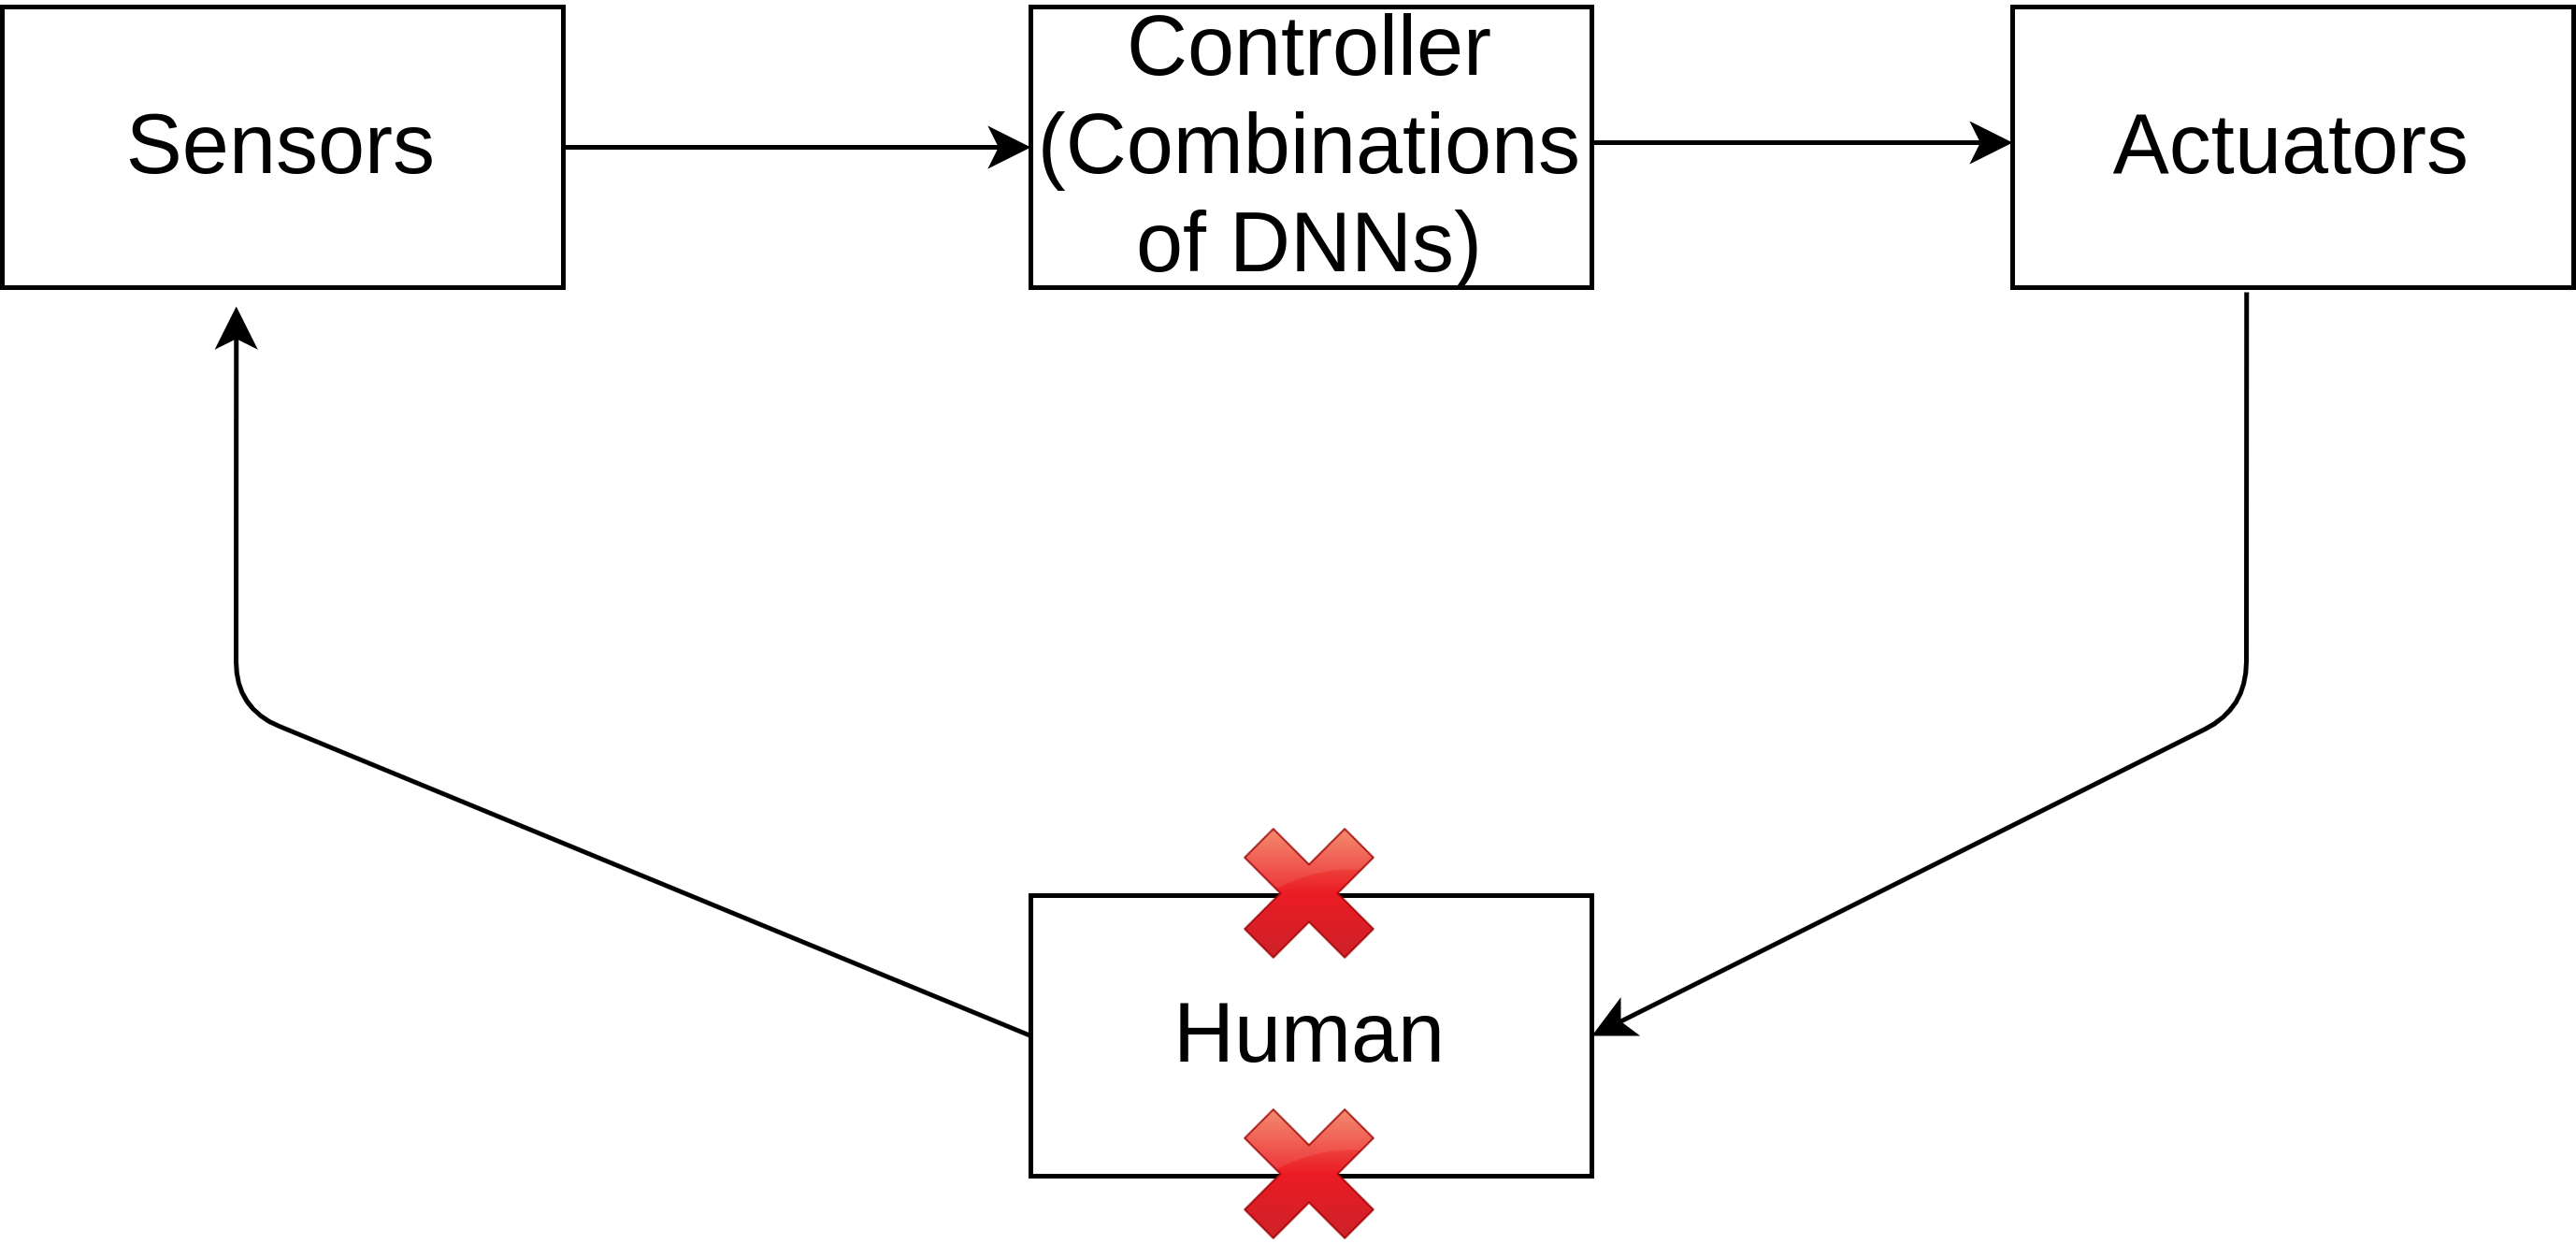
\includegraphics[width=0.7\linewidth]{Images/Systemsdescription}
	\caption{Architecture of a CPS}
	\label{fig:systemsdescription}
\end{figure}

\begin{figure}
	\centering
	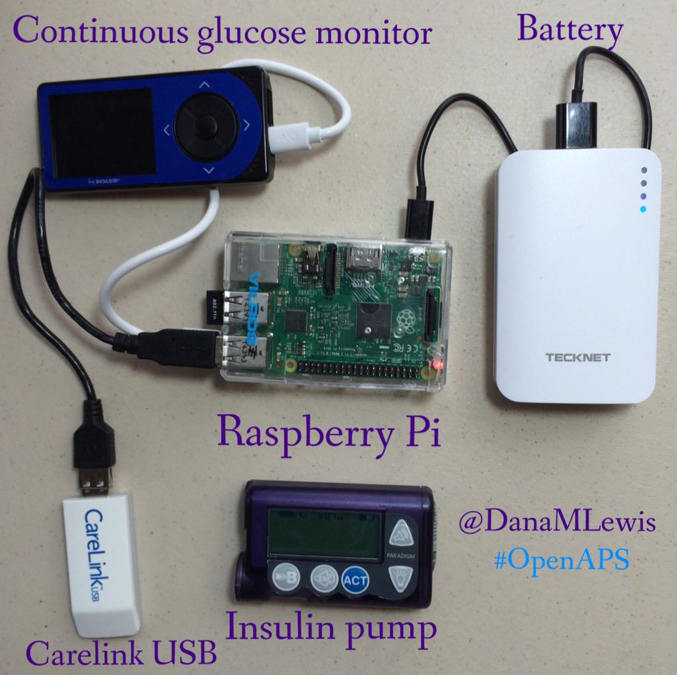
\includegraphics[width=0.7\linewidth]{Images/APSrig}
	\caption{Artifical Pancreas System components \\
		Source: www.openAPS.org}
	\label{fig:apsrig}
\end{figure}



\begin{figure}
	\centering
	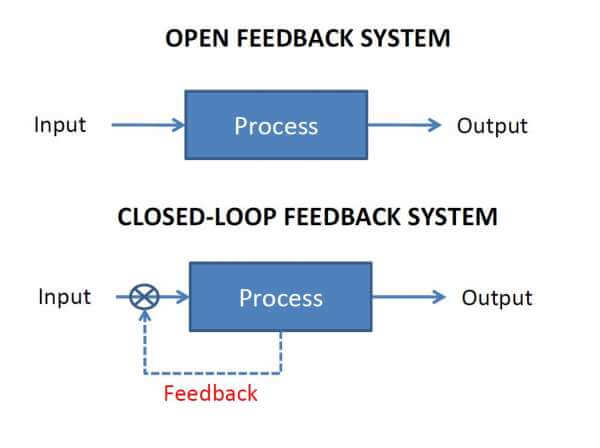
\includegraphics[width=0.7\linewidth]{Images/closedvsopen}
	\caption{General structure of a open and closed-loop systems 
		Source:https://instrumentationtools.com/open-loop-and-closed-loop-animation/ }
	\label{fig:closedvsopen}
\end{figure}


\section{Cyber-Physical Systems}
\ac{CPS} are systems that perform computations in the cyber part to reflect changes in the physical  part.   
As shown in Figure ~\ref{fig:systemsdescription} the sensors and actuators are the physical parts of the system. 
The sensors gather the data from the physical environment and send it to the computational unit. 
The decision is taken at the computational unit which is also the cyber part of the \ac{CPS} called the controller.
The decision is sent to the actuator which then physically performs the action.
The physical and virtual contexts can either be humans in the loop or some automated mechanism.

In an \ac{APS} shown in Figure ~\ref{fig:apsrig}, the sensor is the \ac{CGM} that is attached to the back of a patient to report the blood glucose levels.  
\ac{RPi} is the computational part of the \ac{APS}, and the insulin pump is the actuator. 

There are two types of CPS based on the decision making process: open feedback and closed-loop feedback.
In open feedback systems, 
%there is human intervention during the decision making process. 
as shown in Figure ~\ref{fig:closedvsopen} (top diagram), the human is a part of the loop where he/she keeps track of the decisions being taken by the controller. 
In closed-loop systems, there is no human intervention 
as shown in Figure ~\ref{fig:closedvsopen} (below diagram). 
In the latter case, understanding different types of security attacks becomes a necessity because the automation means that once the attacker has found a way to tamper with the automation mechanism, they can fool the system. 
In the case of stealthy (or subtle) attacks as described in Chapter 3, \karthik{Symbolic ref} 
the closed loop systems are more vulnerable because existing error-detection mechanisms can be reverse engineered and can be used to attack the systems. 

\section{Conventional Controllers for CPS}

A conventional controller takes in the sensors readings and processes the input based on the different sets of differential equations for the controller. 
For instance, a quadcopter contains multiple flight modes in its controller based on the weather conditions such as windy or normal day. 
These modes are important because during windy weather, the decision making model for stable quadcopter flights will be different from a normal weather flight \cite{inbook}. 

Based on the inputs or data collected from the sensors, the appropriate  mode is selected and the decision is calculated. 
Every mode consists of a different set of equations because every mode represents a different scenario.
Figure ~\ref{fig:controltheory} shows a position control system of a quadcopter \cite{inbook}. The input values use the derived version of the equations that are used in decision making. 

\begin{figure}
	\centering
	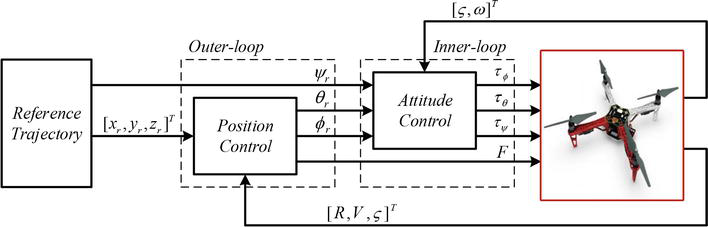
\includegraphics[width=0.7\linewidth]{Images/controltheory}
	\caption{The block diagram of the position control system of the quadcopter.
	}
	\label{fig:controltheory} 
\end{figure}


%How are they modeled
These modes are modeled using classical control theory that is represented as a set of equations designed by domain experts.
For instance, the model for a medical system such as \ac{APS} can be designed only if the specifications are known for the medical system. 
A part of the specifications such as the important parameters (insulin, blood glucose etc. in APS) and their threshold values are be provided by domain (in this case medical) experts. 
Another important aspect for designing control systems is modeling the precise relations between the parameters. 
This is possible in systems such as APS because it is a simpler system as compared to self-driving cars. 
However, designing the precise mathematical relations for systems such as self-driving cars can be tedious \cite{article23}, as we elaborate below.

The move towards DNNs over control theory models for modeling \ac{CPS} behaviour can be justified by the following observations:
\begin{enumerate}
	\item CPS behaviour is controlled using a lot of input data from the many sensors a system might have. The self-learning nature of DNNs lends itself well to model behaviour that is driven by the sensor input. This is easier than formulating the control theoretic differential equations, which need domain and mathematical expertise \cite{Aamir_2013}.
	
	
	To look at a more concrete example, let us turn to a medical system such as \ac{APS}, which uses conventional control theory to build models. 
	Forming the model requires the programmer to be aware of not only the intended system behaviour, but also the mathematical rigor needed to get the desired result. 
	DNNs, on the other hand, can automatically build models with data.
	Training DNNs is implicitly dependent on the quality of available training data, and it is a known problem in the field \cite{jabbar2015methods}. It does not, however, require the system designers to model precise control equations like in control theory.
	\item  There are limitations on the behaviors that can be modeled using the standard control-theoretic approaches. They do not, for instance, work well for building dynamic models \cite{article23}. Building such dynamic models is important in many systems such as in autonomous vehicles, which are essentially composed of multiple interacting control systems. Conventional control systems are not designed to work in an interactive, plug-and-play manner with other control systems because they are built to model only one behaviour. DNNs, by their very nature,  provide this dynamic capability \cite{article23}. 
	Due to the data driven modeling using DNNs, it is relatively easier to build models for autonomous vehicles that have multiple models interacting within them.
	For instance, they contain separate models for image recognition and lane detection that continuously interact with each other to decide the next best course of action.
	
	\item Sarabakha et al. \cite{sarabakha2019online} show that using \ac{DNN} based controller for a quadcopter leads to better decision making in unspecified cases as compared to control theory models.
	This is due to the learning nature of \ac{DNN}s in contrast to the fixed nature of conventional control theory. 
	Hence, in cases when the trajectories or situations are not precisely modeled, the \ac{DNN} comes closer to taking good decisions.
\end{enumerate}




\section{DNN Based Controller}
\label{apsdnn}


%A \ac{NN} is an algorithm that is modeled after the human brain.
A \ac{NN} consists of input, output and hidden layers. 
The layers are built of nodes. Every computation occurs within in a node of a network.
In the base case, there is a single neuron that takes all the inputs to produce an output as shown in Figure 2.5. 
All inputs to the node in Figure 2.5 are summed up, and  passed through an activation function. 
The activation function introduces non-linearity in the network. 
The node determines up to what extent the signal must be progressed \karthik{seems awkward} to calculate the final output. 
The final output depends on the network and can be in binary form or have a value associated with it. 


A \ac{DNN} consists of multiple hidden layers as apposed to our base case  as shown in Figure 2.7.
This is an example of a feed-forward \ac{DNN} which is the simplest type of artificial neural network devised \cite{feedforward}.
In this network, the information flows only forward from inputs, through layers, to outputs \cite{Zell}. 

The classical controller model is being replaced by such DNN based controllers for CPS as shown in  Figure 2.6.
The \ac{DNN} for \ac*{CPS} is trained using the data gathered from conventional control equations. 
One example is the DNN based controller designed by Dutta et al. \cite{Dutta_Others__2018__Robust}. 
Dutta et al. model robust DNN using available patient data to predict the output for an insulin pump.
Their controller design is for providing a data-driven approach for an artificial pancreas system (APS), which is also our first system for evaluation. 

We evaluate two other systems called \ac{CA} systems for unmanned vehicles \cite{7778055} called \ac{HCAS} and \ac{ACAS-Xu}: both \ac{CA} systems are bigger in size (number of nodes and layers) and have a complex architecture in terms of design as compared to \ac{APS}.


%Normalization layers in DNN
\ac{DNN}s also consist of a feature called normalization in their layers. 
This feature exist mostly in \ac{DNN}s as compared to other \ac{ML} models such as decision trees, since \ac{DNN}s involve less feature engineering as compared to other models. 
Feature engineering is an automatic method to extract features from raw data. 
Normalization is a common feature engineering method where all the inputs are brought to standard scale since different set of inputs can be in different ranges. 
This is important in \ac{DNN}s for reasons explained by  LeCun et al.  \cite{10.5555/645754.668382}.
%The first reason is trivial as computations on a bounded range of numbers prevent some numerical inaccuracies and limit the computational power required. The second reason is that some machine learning algorithms can handle that data better when it is normalized. There are several approaches to normalization of the data.
Our other two evaluation systems are aircraft  control management systems \cite{10.1007/978-3-319-63387-9_5} that consist of a normalization layer, 
which we have to consider in our system modeling. 
\subsection{Understanding DNN complexity}
\label{dnncomplexity}
To understand the complexity of \ac{DNN}s we use two criteria
\begin{enumerate}
	\item Size: The size depends on two aspects, the number of layers in a \ac{DNN} and the number of nodes in each layer. 
    The increase in the hidden layers corresponds to more connections and opacity between the inputs and the outputs. 
    The increase in the number of nodes per layer corresponds to more connections between each layer which ultimately increases the opacity of the input and output mapping. 
	\item Architecture: The architecture consists of the the design of the network. 
	For a fully-connected network, every node is connected to every other node in the network, and it contains ReLU or some other activation function to introduce non-linearity.
	Other networks also consist of layers that perform max/average pooling operations. 
	
\end{enumerate}
When we refer to \ac{DNN} complexity in this thesis, we are referring to the differences in size and architecture.


\begin{figure}
	\centering
	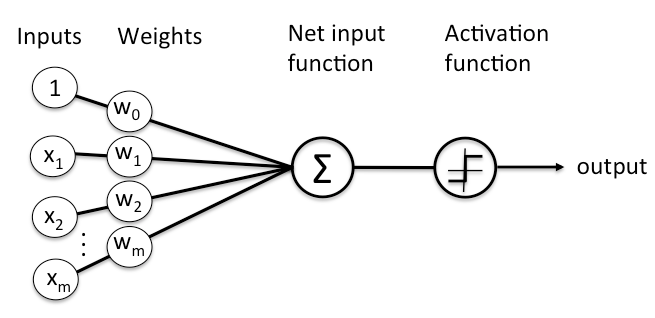
\includegraphics[width=0.7\linewidth]{Images/perceptron_node}
	\caption{Perceptron node  \\ Source: https://pathmind.com/wiki/neural-network}
	\label{fig:perceptronnode}
\end{figure}

\begin{figure}
	\centering
	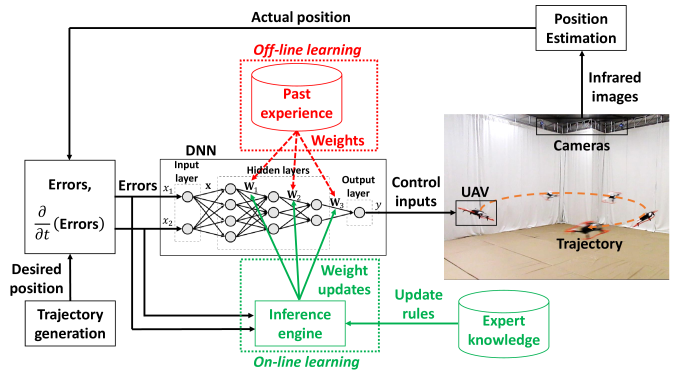
\includegraphics[width=0.7\linewidth]{Images/DNNcontroller}
	\caption{Illustration of how DNN controllers are replacing conventional controllers. The DNN is trained offline using input-output data obtained from different trajectories from a conventional controller. The DNN is shown to perform better than a conventional controller during real-time analysis for decision making.}
	\label{fig:dnncontroller}
\end{figure}

\begin{figure}
	\centering
	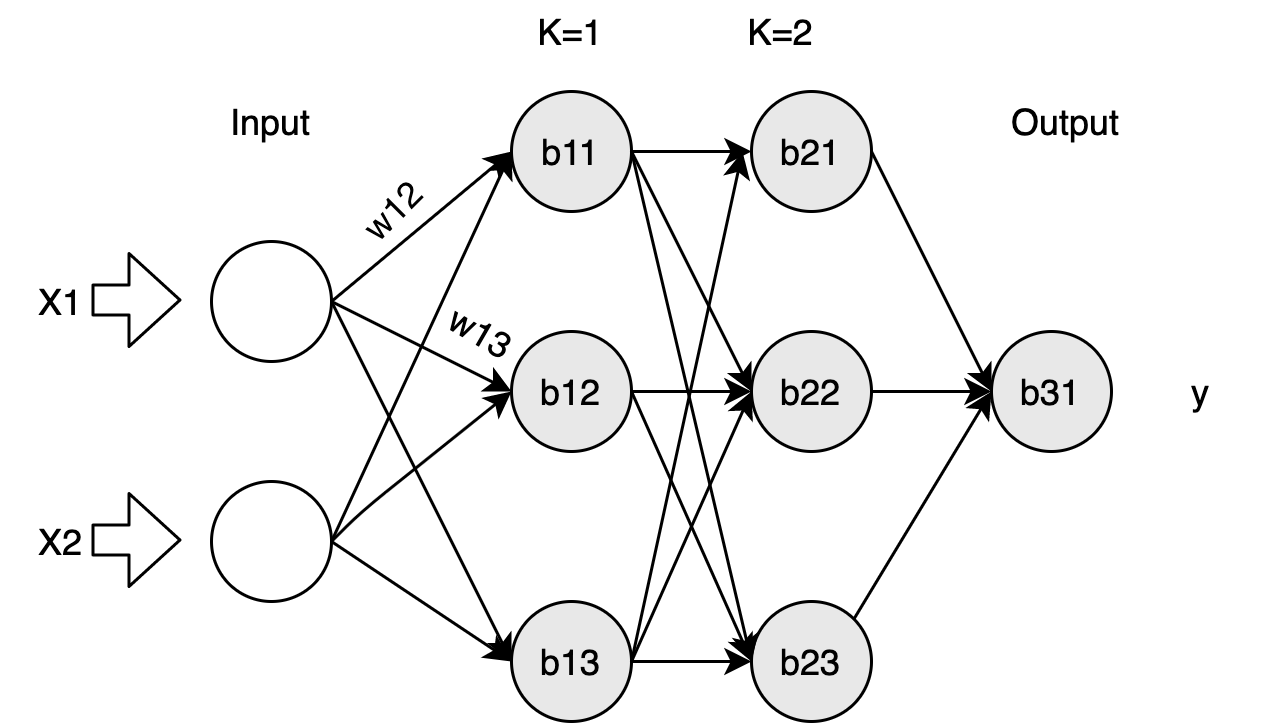
\includegraphics[width=0.7\linewidth]{Images/DNNstructure}
	\caption[DNN structure]{DNN controller structure with two hidden layers K=1,2, two inputs x1 and x2 and one output y. This is an example of a fully connected network.}
	\label{fig:dnn-controller}
\end{figure}

\section{Modeling Mixed-Integer Linear Programming Problems}
\label{milp}
We present a general structure that is required for building a \ac{LP} \ac{MILP} models.
The reason we are introducing the notion of \ac{MILP} is because we use the modeling techniques underlying \ac{MILP} to model \ac{DNN}s and systematically reason about them. 
An \ac{LP} is characterized by the following components. 

\begin{enumerate}
	\item A \ac{LP} contains a set of decision variables, which are the unknown quantities or decisions that are to be optimized. 
	\item The function that assess the quality of the solution is called an objective function or the cost function.
	\item \ac{LP}'s goal is to minimize or maximize the value of an objective function. 
	The decisions that are to be made depends on the requirements, and restrictions of the  system modeled as \ac{LP}.
	\item A solution that satisfies all constraints is called a feasible solution. 
	Feasible solutions that achieve the the best cost function value, depending on weather one is minimizing or maximizing are called as optimal solutions. 
\end{enumerate}


The general form of a \ac{LP} looks as shown in Equations 2.1. 
Values of $c$ denote the objective coefficients, and are often associated with their corresponding decisions minimization problems. 
$x_i$ denotes the set of our decision variables.
$b_i$ denotes the requirements of the constraints. 
A very important point here is that nonlinear terms are not allowed in the model. 
Hence, something as simple as multiplication of two decision variables is prohibited in the model representation. 
\begin{equation}
\begin{aligned}
& \underset{x}{\text{min/max}}
& & c^T x \\
& \text{subject to} & &  Ax \leq b_i \\
& & &  \sum_{i=1}^{n} x_i =1 \\
& & &  x_j, \; \forall j \in N. \\
\end{aligned}
\end{equation}

A \ac{MILP} is a \ac{LP} with a restriction that some of the variables in the model must be integer-valued. 
We define a \ac{DNN} as a \ac{MILP} model due to the complex structure of a \ac{DNN} which we will elaborate more in Chapter ~\ref{evaluation}. 

There are multiple tools that provide an interface to build \ac{MILP} models such as Cplex ~\cite{cplex}, and Gurobi ~\cite{gurobi}.
Both are high-performing tools\karthik{What's a high-performing tool?}; however, we choose Gurobi for our purpose as it was more usable\karthik{Please check}. 



\section{Problem Statement}
\label{problemstatement}

Given a trained DNN with fixed parameters our goal is to understand if the well-known \ac*{FDIA} in classical control theory are also valid in the DNN based CPS. \karthik{Given that we've introduced RFDIA, should we simply say RFDIA here?} \karthik{and to automatically mount them, correct ?}
This leads to two sub-problems as follows.

\begin{problem}
	How can we identify the critical inputs in a DNN?
\end{problem}

\begin{problem}
	What is the smallest perturbation to the critical input(s) that can produce \ac{RFDIA}?
\end{problem}





\chapter{Motivating Example}
\label{ch:Chapter2}
\section{Motivating system: APS}
We use a DNN based Artificial Pancreas system(APS), closed-loop model, by Dutta et al. \cite{10.1007/978-3-319-99429-1_11}  as our motivating example for showing \attack. According to the APS, the patient relies on the model to predict the next dose of insulin to be injected into the body. 

%How is APS constructed?
The APS consists of sensors and an actuator, one that calculates the blood glucose values and one that injects the insulin inside the body respectively. The values from the two sensors are sent to the controller that calculates or predicts the next outcome. The network samples the previous blood glucose and insulin values discretized overtime at every 5 minutes. Such a model whose prediction depends on the data collected previously over time is called a data-driven model. The APS DNN model from Dutta et al. is shown in Figure 1. The DNN for APS is able to create mappings between the insulin and the glucose values that allow for the prediction of future insulin values. The model has 74 inputs in total as shown in Figure 1 where 32 inputs are the glucose and the rest are insulin values collected over a span of every 5 minutes. The DNN layers map these values with each other to predict the next value. 
\begin{figure}
	\centering
	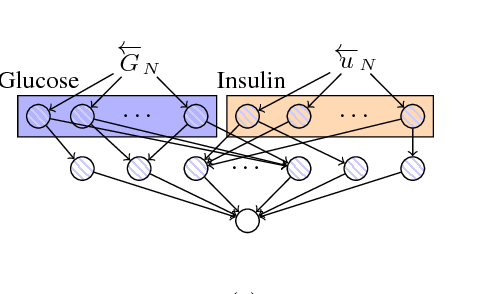
\includegraphics[width=0.7\linewidth, height=0.3\linewidth]{Images/APSDNN}
	\caption[APS DNN]{APS DNN designed by Dutta et. takes in 74 inputs of insulin and glucose. The next layers form connections between the insulin and the glucose to make predictions.}
	\label{fig:apsdnn}
\end{figure}

%Defense mechanisms
The APS DNN has certain defense mechanisms accompanying it. The DNN is accompanied by two DNNs that are trained to calculate the upper and the lower bounds to keep a check on the output prediction. In APS there is one output value that predicts the next outcome. Initially the expected output value is 140, after the attack the attacker changes it to 190. Due to the accompanying detection mechanisms, the attack will get detected. The range of acceptable output should be between 120-160. Hence, we want to perturb our inputs such that the output value is below 160 but much higher than 140. This is our motivation for designing an automatic attack synthesis mechanism. 

%This accompanying mechanism ensures that if the output value was supposed to be 140, does not change to 190 due to some malicious means. If the values don't lie within the bounds alarms are triggered. Our goal is to attack the system within these bounds and still cause some damage. 
%What is our goal
Since APS is a closed-loop system there is no human oversight. Consequently, it is important to ensure that the system is robust against ripples. We discuss a motivating attack below. 


\section{Attack Model}
CPS consist of the physical and the cyber-part. The physical part consists of components such as sensors and actuators. The attacker's goal is to manipulate the sensor measurements to conduct FDIAs without triggering alarms. The attack is conducted in a stealthy way such that the compromised inputs lie within the threshold ranges. 
%Based on our motivating example of APS, perturbing the inputs slightly and causing ripples ensures that no alarms are triggered. This leads to the wrong prediction of the outputs. However, since the deviation is so small, it is not observable in a closed-loop system by inbuilt error-detection mechanisms. 

We assume that the attacker has the following capabilities:
\begin{enumerate}
	\item The weights and bias for the DNN are available through one-time read-only access. There are multiple models that are open-source such as openAPS \cite{openAPS}. There are multiple reverse-engineering mechanisms \cite{10.1145/3195970.3196105} that allows one to infer the DNN models.  
	\item Has one-time access to the system to CPS since the attacker cannot keep injecting false data every five minutes (the data is collected from sensors as explained in the Motivating example section).
	%\item Can tamper \smi{add 'with' here} only the physical parts of the CPS such as the sensors based on her targeted attack. 
	\item The attacker does not modify the code but only the inputs to the model.
\end{enumerate}

\subsection{Dumb attacker}
The first way to attack the system would be to change all the 74 values that are the inputs to the DNN. If all the inputs are changed, the final output prediction is going to be wrong. The problem in this particular scenario is that these inputs are collected every five minutes from the sensors attached to the patient as explained above. This means that the attacker will have to conduct false data injection every five minutes when the data is being collected to cause a change in the output. Doing this is not feasible in a practical scenario and hence, the attacker needs a better way of attacking the system. 

\subsection{Smart Attacker}
A more sophisticated approach for the attacker to attack the system would be by perturbing one or two inputs out of the 74 inputs that cause a change in the output. There are two ways to proceed when the attacker tries to change just one or two inputs at a time. 

\subsubsection{Attack 1}
The attacker can randomly choose two inputs and perturb them by huge amounts. This will indeed cause a wrong output prediction. However, if the input is perturbed by very large amounts, the error detection mechanisms will recognize that there is an anomaly. To prevent this the attacker can choose to perturb the two inputs by small amounts. However, perturbing any two random inputs by very small amounts might not necessarily lead to a wrong output prediction.

\subsubsection{Attack 2}
Adding one more layer of sophistication, the attacker supposedly knows the critical inputs or the inputs that on perturbing can lead to wrong predictions. This will be a more targeted approach for attacking the system since the input selection will not be random. Here not knowing the precise amounts by which the critical inputs should be perturbed can lead to an unsuccessful attack. If the perturbation is too high it will trigger the error-detection mechanisms and if it is too low then it will not affect the output. 
\subsubsection{Attack 3}
The most sophisticated means for an attacker to attack the system would be to know precisely which inputs to perturb and by what amounts such that the output prediction is wrong. To do so, the attacker needs an advanced technique that in limited time finds the critical inputs (as we call them) and also the small perturbations that can ensure a wrong output prediction. 

We consider Attack 2c for our evaluation systems and develop a technique called \tool that can automatically synthesize such attacks in a limited amount of time. 



%The attacker does not have write-access to the operating system in the hardware. If the attacker has read-access then she can easily change the code, however, we assume that the attacker can only tamper through physical means.
%We assume that there are error-detection mechanisms that are deployed on top of the APS model that does not allow the attack to be successful if there are huge deviations observed from the input. The final and very important assumption is that the attacker has a limited amount of time to synthesize the attacks and then mount them after the first read access.
%Hence, the attacker needs to find the correct ranges of the inputs to conduct the attack. 





%We use an Artificial Pancreas System(APS) as a running example to motivate the problem and illustrate our technique. This is an example of a safety-critical CPS that uses DNNs.\karthik{Please check}
%A patient using an APS relies completely on the closed-loop model of the APS\cite{10.1007/978-3-319-99429-1_11}. She trusts the model to monitor the body and deliver the right amount of insulin. %However, the APS does not consider side-channel attacks that can be conducted due to the CPS's interface and the presence of DNNs. \karthik{This should be in the Threat model section, not here}
%\karthik{Can you provide a brief description of the APS system, including the role of the DNN? - this is explained in the next paragraph}
%\karthik{You never talk about the DNN through}

%The attackers' goal is to change the inputs slightly such that the amount of insulin to be injected every time is more than the original amount that is supposed to be delivered.
%\karthik{What's the actual amount - the one that is supposed to be delivered when there is no attack}. 
%We want the inputs to be only minutely perturbed such that there is some output deviation observed from the original output. 

%There are two parts to conduct an attack. Since this is a data-driven attack \karthik{What's a data-driven attack? Either cite or define}, 
%the DNN predicts the output by taking in the inputs over time \karthik{What does over time mean?}. Hence, the network has 74 inputs in total \karthik{How does this follow?}. 
%Changing all 74 inputs is not feasible in a practical setting \karthik{What would it entail for the attacker to do this?}. 
%Hence, to conduct a successful ripple attack \karthik{We didn't say the attacker wants to conduct a ripple attack so far}, 
%the attacker needs to first find the critical input and perturb them by specific amounts \karthik{input or inputs}. 
%We provide a technique and automated tool for finding the critical input and further by finding the smallest possible perturbations to those inputs to cause a ripple.
%\karthik{Again, this is already explained in the intro - we need to be specific here} 

%Our proposed synthesized attack can ensure that the inputs are changed in a way that the output always lies within the upper and lower bounds set as constraints for the safety settings for the system. A consistent deviation from the actual value of insulin leads to damage to the patient.  \cite{ZHANG2019403}.

%\karthik{This section is very poorly written - please rewrite it}
%\aarti{Is it easy to understand this? - This is very important to highlight the importance of this work. - there are three models that are deployed together, hence we have to very carefully craft the attacks. }
%\include{Rippleattacks}

%\chapter{Challenges}
We face  the following challenges during  the design of the technique. 

\section{ Mapping DNNs to MILP}
What do I want to say ?
- DNNs when with brute force take time since we cannot keep solving every solution space. 
- Define DNN solution space mathematically
- 
DNNs are complex algorithms 
It is is difficult to use b


\section{\textbf{C1}: Finding the critical inputs}
For the sophisticated attacker to conduct \attack as described in Chapter 3, the attackers require two vital pieces. The first one is finding the critical inputs. We explain this with our motivating example of the APS system from Chapter 3. APS has 74 inputs. It is not feasible to change all inputs by False Data Injection since the attacker will have to keep changing the inputs every five minutes. Therefore, if the model architecture is known to the attacker, the goal of the attacker is to quickly locate the critical inputs. Given this is a DNN based system, it is not possible to test it for every possible input-output combination in minimal amount of time to figure out the patterns for finding the critical inputs. 

\subsubsection*{Selecting  the automated technique}
The first part is choosing a technique that allows the attacker to model a DNN and find the critical inputs through the modeling. There are multiple means of modeling the DNN, some of which are using SMT solvers, symbolic execution, MILP and many more. 
Our goal is twofold: 
\begin{enumerate}
    \item generality
    \item scalability
\end{enumerate}

APS has a  feed-forward architecture with 74 inputs whereas the other systems on which we test our technique have completely different architectures as can be observed from Table 6.1 in Chapter 6. This is due to the difference in the application domain. APS is a medical system that is much easier to reason about as compared to our other test systems that are collision avoidance systems for air traffic control management.
APS has two layers and is the smallest system that we tested our technique for but we want our technique to be valid for much bigger systems as shown in Table 1. We show that MILP fulfills these two criteria by providing us generality and scalability. 


\section*{\textbf{C2}: Finding the input perturbations}
After locating the critical inputs, the next part of the challenge is to find the correct perturbations that can lead to ripples in APS. Based on Section V formulation, if the inputs in equation (1) ($x$) are perturbed by very small amounts, the effects are not observed in the final output due to the existence of K layers in the system and the ReLU activation function as shown in (3). There is not a linear mapping between the inputs and the outputs and hence, it is a challenging problem to find just the right perturbations. We show how we tackle this in our methodology using MILP. To find the correct perturbations for \attack, we run into the following challenge. 

\subsubsection*{Designing \attack specific cost function and selecting the range intervals for inputs and outputs. }
APS DNN is an architecture where K (the number of hidden layers) is 2, and the vector input $x$ consists of 74 inputs. Our attack model is that we want to perturb the inputs by the least amounts and cause deviations in the output that are not above a certain threshold. The threshold value is determined based on the specifications of the system as described in Section III. 
 Hence, our challenge here is how we design our cost function and add a range limit to the perturbations to ensure that the perturbation does not exceed the input values above or below the bounds. 


\chapter{ReLUSyn}
\label{relusyn}
In this section we explain the inner workings of our tool ReLUSyn. 
There are two parts to this; we first explain our approach and our algorithms that are used for the synthesis, and we then talk about our tool \tool that implements the algorithms and synthesizes the models and attacks. 
We show how fully connected feed-forward \ac{DNN}s can be formulated as \ac{MILP} models. 
We use a generic representation and describe the modeling of cost functions that are used to generate \ac{RFDIA}.
We then show how this allows us to identify critical inputs and find the perturbations. 
We finally explain how we map this to real systems.
We also include a section on how ReLU (the non-linear activation function) might be modeled internally by MILP solvers based on work by Fischetti et al. \cite{fischetti2017deep}, where they propose a 0-1 MILP model for DNN modeling.
This section is included for completeness as the solver we use for our evaluation is able to handle the $\max$ function automatically.

\begin{figure}
	\centering
	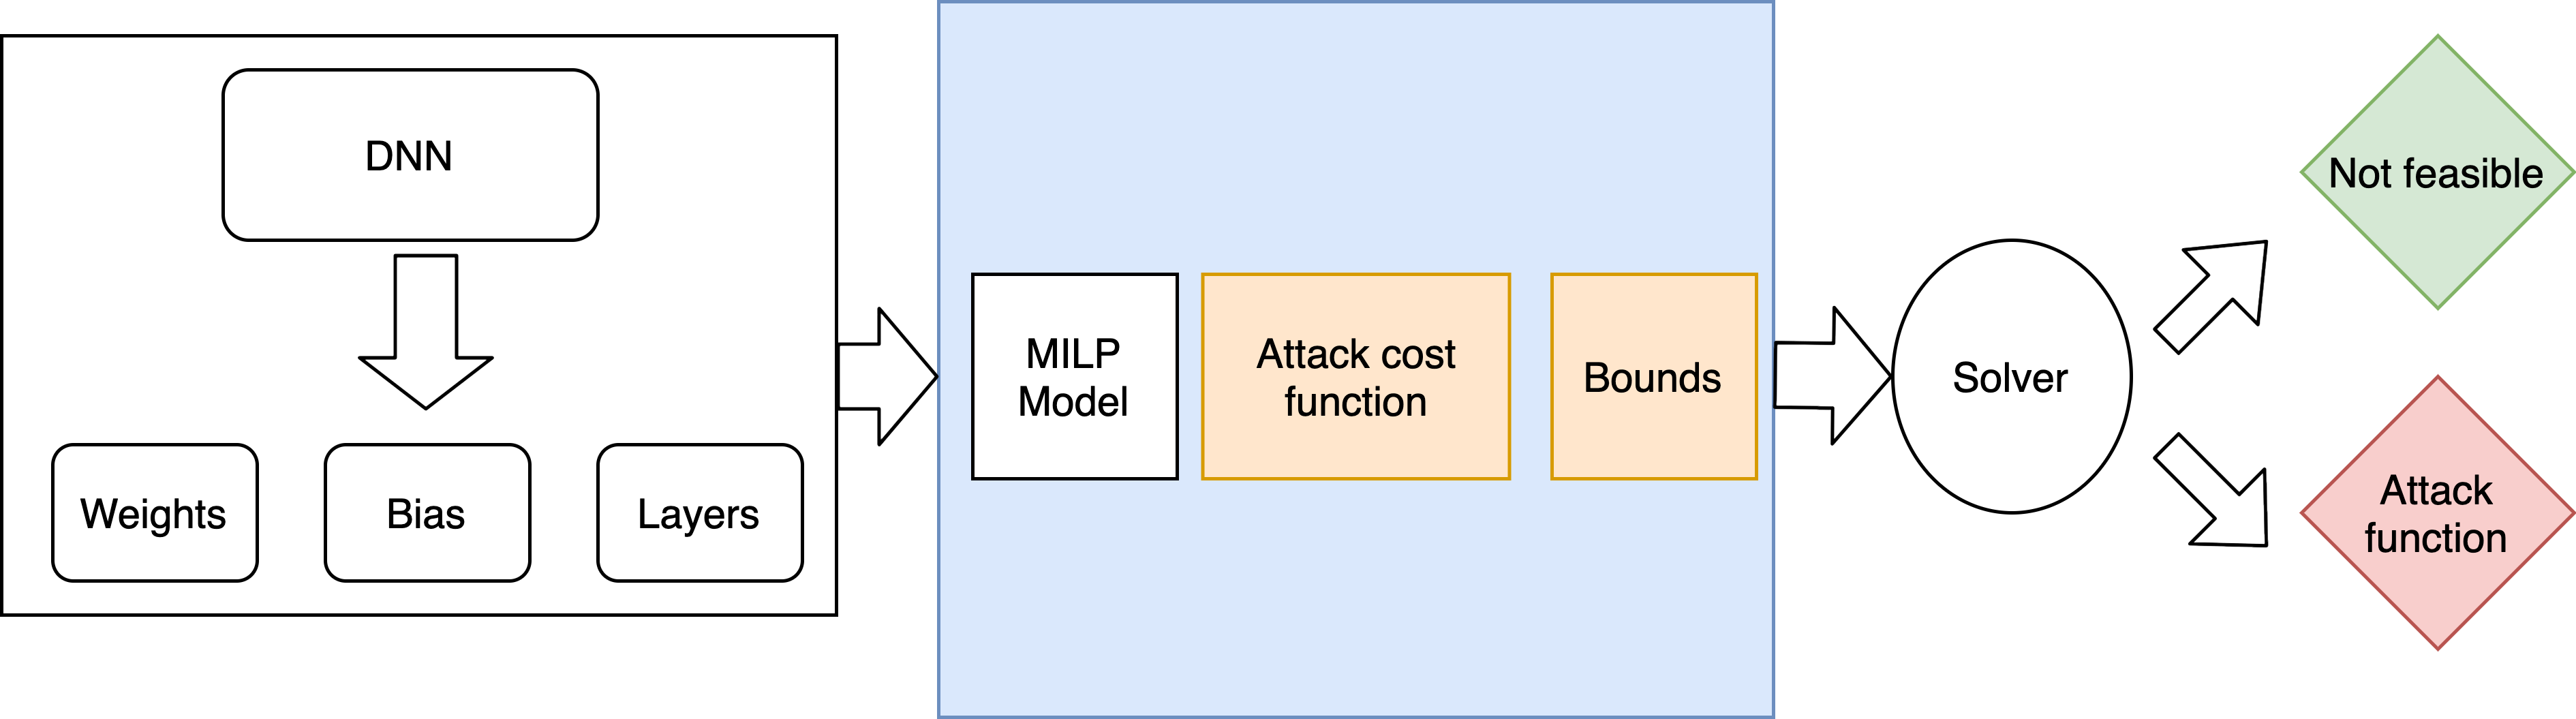
\includegraphics[scale=0.1]{Images/Methodology}
	\caption[Methodology]{The rounded boxes depict the information provided by the users and the sharp corners is the information provided by us that integrates the first layer into the solver layer.}
	\label{fig:methodology}
\end{figure}

\begin{figure}
	\centering
	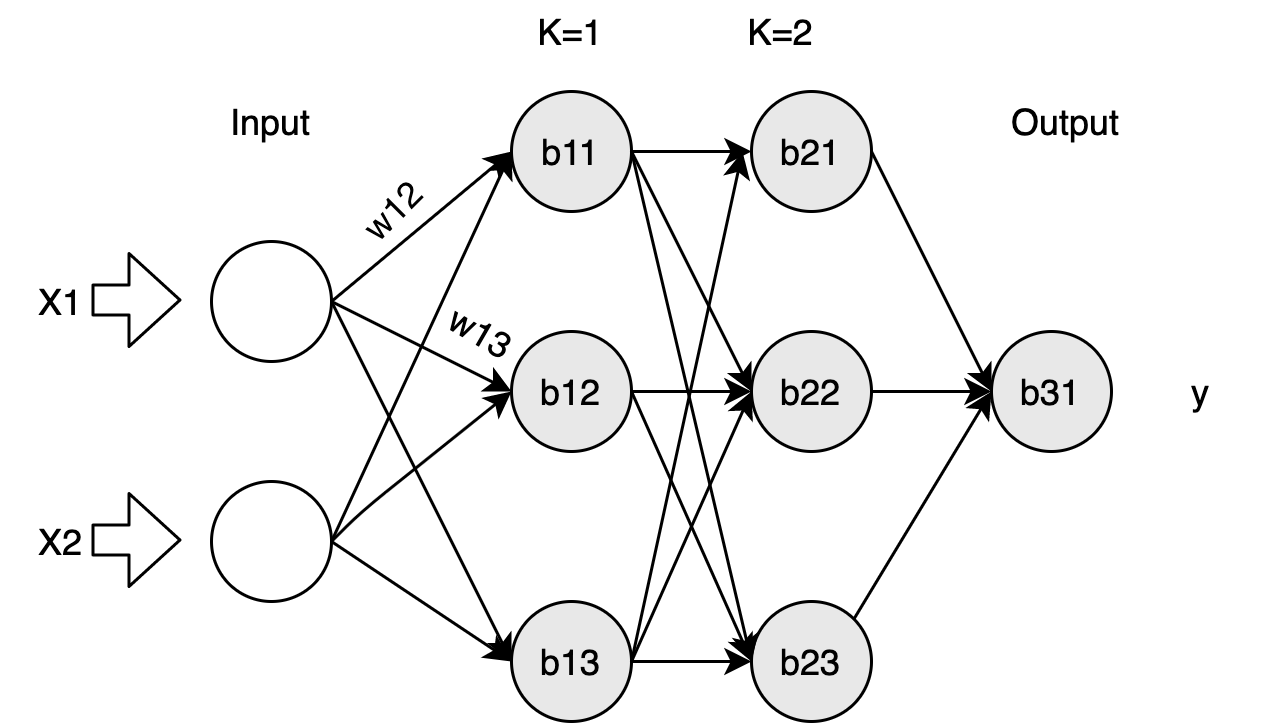
\includegraphics[width=0.7\linewidth]{Images/DNNstructure}
	\caption[DNN structure]{DNN controller structure with two hidden layers K=1,2, two inputs x1 and x2 and one output y. This is an example of a fully connected network.}
	\label{fig:dnn-controller}
\end{figure}


\section{ReLUSyn: Overview}
ReLUSyn is the tool that models our approach, and allows the attacker to generate \ac{RFDIA} attacks directly from the \ac{DNN} model. 
Our technique is shown in Figure ~\ref{fig:methodology}.
The \ac{DNN} is made available from the systems which can be directly passed through \tool. 
It automatically synthesizes a \ac{MILP} model from the \ac{DNN} model which also contains the input value bounds.
The attacker can specify a cost function if they possess the relevant domain-specific knowledge to make such a decision. 
The cost function determines the kind of attack to be launched on the system.
\karthik{Please say who does the synthesis in the next 2 sentences}
Everything inside the blue box is automatically synthesized in Figure ~\ref{fig:methodology}.
The cost function and bounds have a plug-gable \karthik{no hyphen} functionality. 
Everything inside the blue box is automatically synthesized. \karthik{Duh ! Didn't you just say this ?}
The orange parts can be easily changed to extend the technique for different systems and applications in the future. \karthik{What are these parts again?}
The models along with the cost functions and bounds are passed through a MILP solver; the solver finds an optimal solution for the MILP model, and this optimal solution corresponds to an attack. If the solver determines the model is infeasible, then no attacks exist.
Each feasible solution of the model corresponds to a particular attack \karthik{How's this different from what you told me 2 sentences back?}
and the optimal solution corresponds to the preferred attack as specified by the user's cost function. We discuss the concept of using cost functions to launch specific attacks later in this chapter.
	
\section{DNN formalism}
We follow the formalism based on the general architecture that we explain in Chapter ~\ref{background}. 
The \ac{DNN} controller maps the inputs that are the $x1$ and $x2$ to the output $y$ as shown in  Figure ~\ref{fig:dnn-controller}.   
We now begin with the formal modeling of the \ac{DNN}.


%Formal modeling of a DNN for later use when explaining the modeling in MILP  
The architecture can be represented as a function F defined as $F: X \rightarrow Y$ where the inputs X are mapped to the output Y and are composed of multiple layers. 
We consider \ac{DNN} to be made up of $K + 1$ layers, numbered from 0 to K.
Layer 0 %does not really exist since it 
is the input layer of the network, while
the last layer K corresponds to the output of the \ac{DNN}.
Every individual layer in the \ac{DNN} $k$ $\epsilon$ $\{0,1,....,K\}$ consists of $n_k$ nodes or neurons in the network.
Each neuron has a bias associated with it. 
Every neuron from the previous layer is connected to every neuron in the next layer. 
The neurons are labeled starting from $1$ to $n_k$ in the network. 
We denote every neuron by $NODE(i,k)$ which corresponds to the $ith$ node for the layer k. 

We denote the output vector of the layer $k$ as $F_k(x)$.
The output for every $NODE(i,k)$ denoted as $F_{ik}(x)$ where $i$ $\epsilon$ $\{0,1,....,n_k\}$ 

The output for layer 0 is represented as $F_k(0)$.
For every layer $k \geq 1$ the output vector is represented in Equation ~\ref{1}. 

\begin{equation}
\label{1}
\begin{aligned}
F_k(x) &= \upsigma(W^{k-1}x^{k-1} + b^{k-1}) \\
\end{aligned}
\end{equation}

where $\upsigma$ represents the activation function being used in the DNN under consideration. 
There are multiple types of activation functions with different modeling capabilities, such as ReLU ($f(x) = max {0,x}$) as shown in Figure 	\ref{fig:relubreakdown} and logistic (or sigmoid) activation function $f(x)=1/(1+ exp(-e))$.
\tool focuses on using Rectified Linear Unit (ReLU) since it is one of the commonly used activation functions in \ac{DNN}s as Krizhevsky et al. \cite{10.1145/3065386}. 
Hence, our equation now \karthik{as opposed to in the past ? Please avoid words like now} looks something like where, for a vector $x$, \texttt{ReLU}($x$):= $\sum_{i=1}^{n} e_{i}\max(0, x_{i})$ (per layer).



\begin{equation}
\label{2}
\begin{aligned}
F_k(x) &= ReLU(W^{k-1}x^{k-1} + b^{k-1}) \\
\end{aligned}
\end{equation}

Since a network consists of multiple layers, the general \ac{DNN} representation looks like a composition function as shown below. 
\begin{equation}
\label{3}
	\begin{aligned}
	F(x) &= F_K \circ F_{K-1} \circ F_{K-2} ....... \circ F_1(x),    \\
	or \\
	F(x) &= F_K ( F_{K-1}( F_{K-2} .......  (F_1(x)))),    \\
	\end{aligned}
\end{equation}

%This ends  our \ac{DNN} formalism. In the next section we use the formalism to create a \ac{MILP} model. 

\section{MILP Model}
The ReLU activation function cannot be modeled directly by MILP solvers. 
This section presents an
equivalent formulation that is accepted by such solvers, which we use to locate critical inputs and find the minimum perturbations as explained in ~\ref{problemstatement}. 
The solver we use, Gurobi, handles this conversion
internally without exposing the details to the user. 
However, we include the details for the purpose of completeness.

 To create a \ac{MILP} model, the essence lies in studying the basic scalar equation that describes the \ac{DNN} architecture. 

\begin{equation}
\label{4}
\begin{aligned}
x &= ReLU(w^Ty + b) \\
\end{aligned}
\end{equation}
 

We cannot apply the $f(X) = \max(0, x)$ operator directly because it is non-linear. 
Instead, we can rewrite the equation given above as follows:

\begin{equation}
\label{5}
\begin{aligned}
w^Ty + b = x - s, x \geq 0, s \geq 0 \\
\end{aligned}
\end{equation}

The reason we represent it as in Equation ~\ref{5} is to first separate the equation from its non-linear component;  ReLU activation function is the non-linear part of Equation ~\ref{4}.
$s$ in Equation ~\ref{5} translates the ReLU activation function to a linear representation. 
We make this division so that we can reason about the non-linear activation function separately from the actual equation. 

As explained in Figure \ref{fig:relubreakdown}, the ReLU function can be broken in two parts, namely positive and negative parts which is termed as piecewise linear.  
To implement the piece-wise linear behavior, we define an activation variable $ac$ that imposes the logical implications. 
The choice to use different symbols was made in the interest of clarity. The equation in this rewritten form is linear, and it does model ReLU functionality  correctly as $x$ will always be non-negative. 
The problem with this formulation is that it does not admit a unique solution. One way to account for this is to add indicator constraints of the form shown below. 
Modern MILP solvers can handle these constraints directly.

\begin{equation}
\label{6}
\begin{aligned}
ac =  1 \rightarrow x \leq 0  \\
ac =  0 \rightarrow s \leq 0  \\
ac \in \{0,1\} \\
\end{aligned}
\end{equation}

The $x \leq 0$ constraint in conjunction with $x \geq 0$ forces $x$ to zero. The other case forces $s$ to be zero.
This opens the door for a formulation that leads to unique solutions for $x$ and $s$ while enforcing the constraint $x \geq 0$.
The uniqueness may be achieved by adding a regularization term in the objective function that encourages most entries in $ac$ to be zero.
Extending this scalar example to the DNN case leads to a \ac{MILP} model of the form:
\begin{equation}
\label{7}
\begin{aligned}
& \underset{}{\text{min/max}}
& &  \sum_{k=0}^{K} \sum_{i=i}^{n_k}F_{jk}(x)   + \sum_{k=0}^{K} \sum_{i=i}^{n_k}F_{jk}(z)  \\
\end{aligned}
\end{equation}
%ReLU
ReLU constraints
\begin{equation}
\label{8}
\begin{aligned}
& \text{subject to} & &  \sum_{j=0}^{n_k} w_{ij}^{k-1}x_{j}^{k-1} + b_i^{k-1} = x_i^k - s_i^k  \\
& & & x_i^k \geq 0, \\
& & & s_i^k \geq 0 \\
& & & ac_i^k  \epsilon  \{0,1\} \\
& & & ac_i^k  =  1 \rightarrow  x_i^k \leq 0  \\
& & & ac_i^k =  0 \rightarrow s_i^k  \leq 0   \\
\end{aligned}
\end{equation}

Upper and lower bounds for range analysis
%Lower and upper bounds on the model
\begin{equation}
\label{9}
\begin{aligned}
& & & lb \geq x_i^k \geq up, \\
& & &  lb \geq s_i^k \geq up \\
& & & lb \geq z_i^k \geq up, \\
\end{aligned}
\end{equation}


We have divided our \ac{MILP} model in three main parts. 
Equation ~\ref{7} represents the cost functions that are to be minimized or maximized.
These cost functions are different for different applications.  
We will show in the next section how we model cost functions for \ac{RFDIA}
attack synthesis. 

Equations ~\ref{8} represents the ReLU modeling for each layer in the network. 
We showed in Equation~\ref{6} how we can represent ReLU units as a set of linear constraints in \ac{MILP} solvers. 
We expand on it and apply it to all the layers in the modeling. 

Equations ~\ref{9} add lower bounds ($lb$) and upper bounds ($up$) in the  model for different variables that we will  require to add limits to our search space.  
These will be 0 and $+\infty$ respectively except for the first input layer
where the bounds would depend on what is valid input for the DNN application.

Our MILP modeling applies the $f(x) = \max(0, x)$ operation directly to the output of layers because our MILP solver linearizes this internally when solving the model.
This section illustrated how the solver could be handling this linearization internally. The next section describes how we build our model.




\begin{figure}
	\centering
	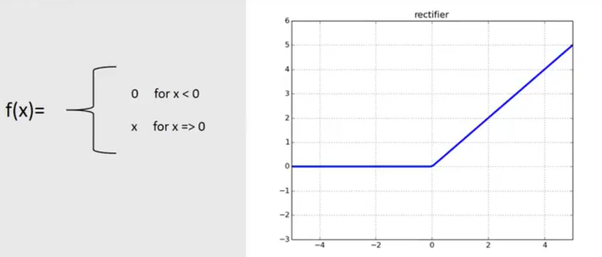
\includegraphics[width=0.7\linewidth]{Images/ReLUbreakdown}
	\caption{ReLU can be broken down into two linear units as shown in the figure for x $<$ 0 and x $\geq$ 0. This allows us to easily map the DNN equations in MILP models by breaking down the non-linearity inducing function.}
	\label{fig:relubreakdown}
\end{figure}

\section{Building the model}
\label{section:attacks}

As part of \tool, we provide automated attack synthesizers for the Artificial Pancreas System, Aircraft Collision Avoidance systems ACAS Xu and Horizontal CAS. 
As an example, we use an \ac{APS} shown in \label{fig:toyaps}, which consists of two sensor inputs that predict the amount of insulin as the output at some time $t$. 
\begin{figure}
	\centering
	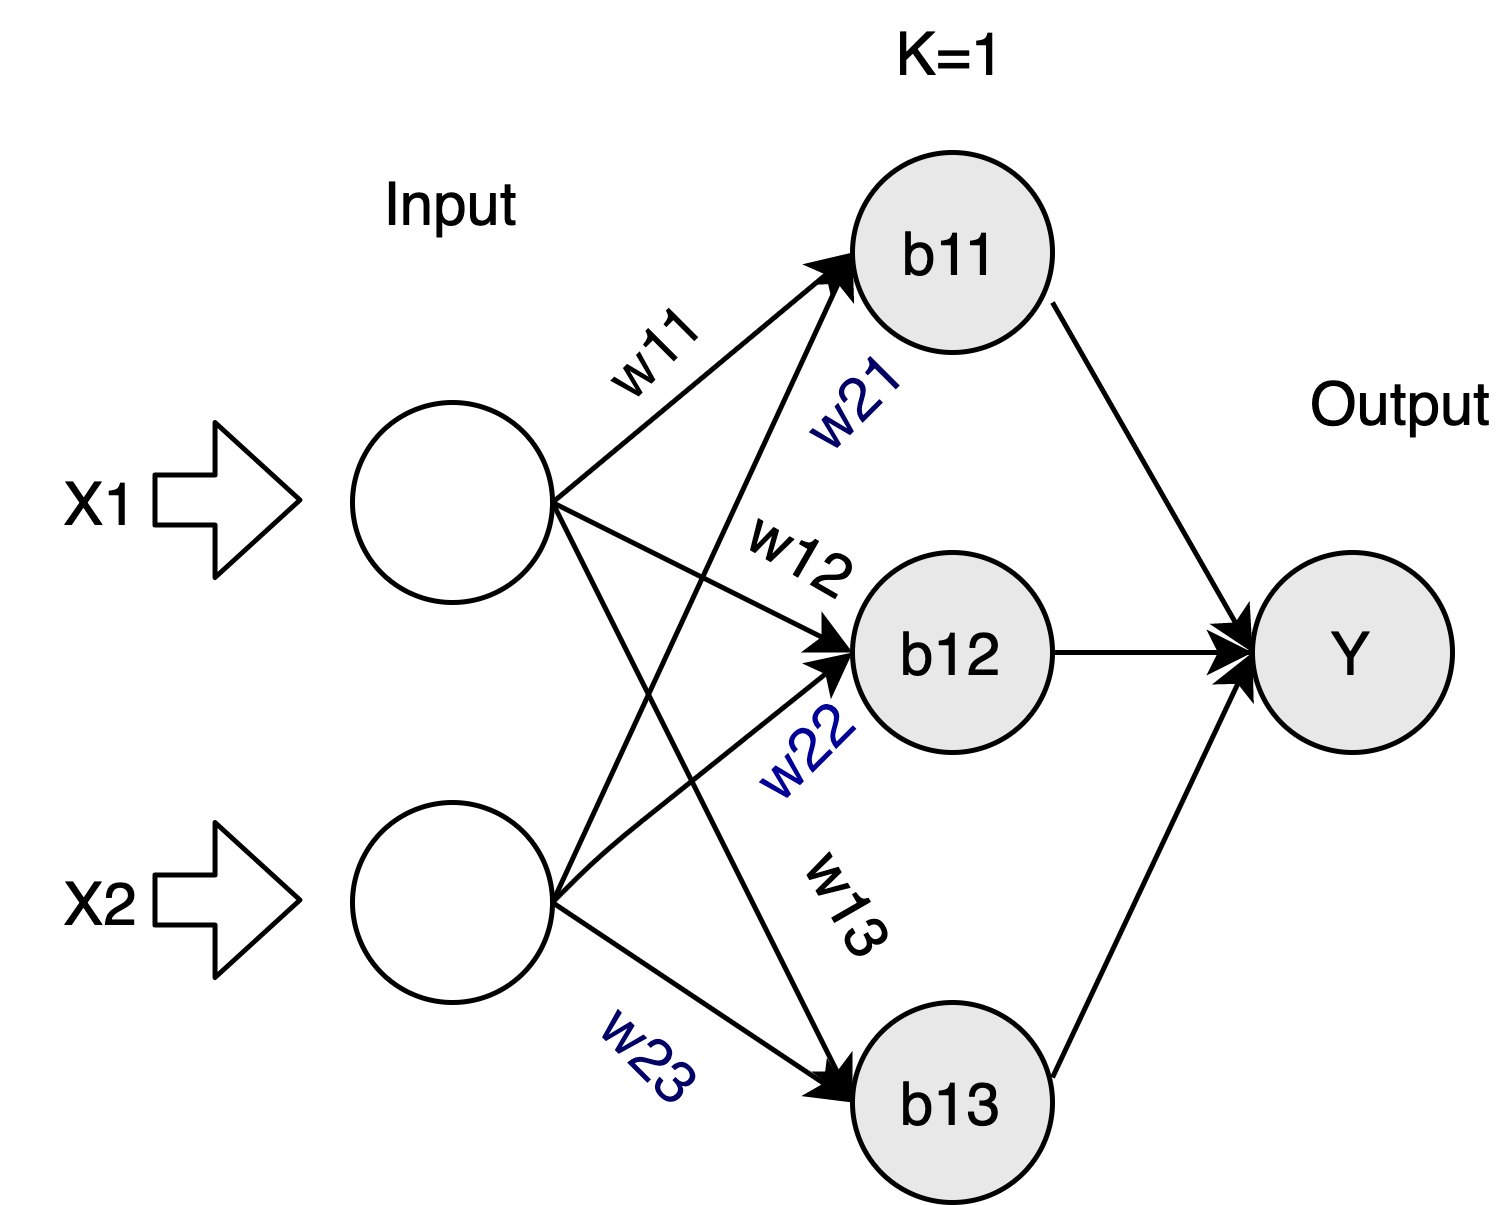
\includegraphics[width=0.7\linewidth]{Images/ToyAPS}
	\caption[APS]{APS that takes in two inputs which we consider as the sensor values from the human. It predicts the amount of insulin to be injected at some time based on the sensor inputs.}
	\label{fig:toyaps}
\end{figure}


\begin{algorithm}
	%\DontPrintSemicolon % Some LaTeX compilers require you to use \dontprintsemicolon    instead
	\KwIn{weight matrices, bias vectors, num\_layers, num\_neurons}
	\KwOut{DNN input, DNN output}
	Take the weight, bias, number of layers, and the number of neurons per layer. \\
	
	\textbf{Model}, \linebreak
	%\renewcommand{\labelenumi}{(\Roman{enumi})}
	%\begin{enumerate}[noitemsep,nolistsep]
	%\item
	(I) For every layer $k$ (with weight matrix $W_k$ and bias vector $b_k$), $output_k = W_k * input_k + b_k$
	\linebreak
	%\item 
	(II) Applying activation function to every layer's output,
	\linebreak
	Constraints: $ReLU\_output_k = max(0, output_k)$ (component-wise) \
	\linebreak
	The final layer's rectified output is the DNN output.
	
	\caption{Modeling neural network in MILP}
	\label{algo:b}
\end{algorithm}


The system can be represented as a MILP model through pseudo-code in Algorithm ~\ref{algo:b}. 
The model generated by this procedure is directly accepted by Gurobi (the solver we use for our experiments).
This converts the neural network structure into a set of linear equations that can be mapped directly into a back-end MILP solver.

An interesting point to note is that the DNN input is an output of Algorithm  ~\ref{algo:b}. 
This is because our procedure does not require an input to the DNN, as the resulting model can be solved to produce a valid input-output pair.
 Bounds can be enforced on the input variables by the user to ensure only
valid inputs are generated by the MILP solver. 
This is a positive consequence of using a constraint solving approach.
 The attacker does not need to have an input in hand when trying to compromise the system using \tool. 
 It also means that we can enumerate many such input-output pairs by repeatedly solving the model,
and adding constraints to exclude previously seen solutions.

This is the general algorithm for converting any \ac{DNN} into a \ac{MILP} model. 
The difference in our evaluated systems and this system is only the difference between the number of layers and nodes in each layer that can be easily extended.
Our \tool  takes in a \ac{DNN} and automatically synthesizes \ac{MILP} models for it. 
Following the same algorithm, we successfully synthesize models for \ac{APS}, \ac{ACAS-Xu}, and \ac{HCAS} within a minute. 

\begin{equation}
\label{10}
\begin{aligned}
x &= ReLU(w^Ty + b) \\
\end{aligned}
\end{equation}
Equation ~\ref{10} represents an \ac{APS}. 
We convert the equations above into a MILP model as shown in Algorithm ~\ref{algo:b}. 
Every layer is initially modeled as a linear equation. 
The activation function is represented as piecewise linear.
Our approach will work for any representation of a piece-wise linear function contingent on the assumption that a non-linear function can be broken down into linear components.
Since we have abstracted away the details that represent non-linearity, the future work\karthik{Do you mean you would consider this in future work?} would be representing non-linear functions as linear functions. 
 However, in our work, we focus on ReLU as explained in ~\ref{problemstatement}

\section{Modeling cost functions for attacks}
\label{section:costfunction}
%Why is modeling cost function important
Now that we have formulated the DNN as a MILP model, the next step is to add a cost or objective function to launch a specific kind of attack. 
This function allows the user to specify which inputs should be perturbed to generate a ripple.

In our \ac{APS}, we have two inputs $x_1$ and $x_2$ that map to an output $y$. 
To conduct \attack, the goal is to change the inputs in a way that the alarms are not triggered, and yet it leads to an output change as we explained in Chapter ~\ref{attack}. 
These small changes lead the system to end up in a bad consequence eventually. 
In \ac{APS}, every small increase is a bad consequence of the system. 
Since the output determines the amount of insulin to be injected inside the body, small increases in the output \karthik{hanging sentence}.
Therefore, the attacker's goal is to change the output to $y'$, where $y' = y + a$. $a$ is some constant. 

%She needs to find the deviations in the input that would help her to change the outputs. 
However, the catch here is that the inputs perturbations should be very small such that the new input now provides her the output $y'$.  
The reason she wants the input perturbations to be small is that there are accompanying neural networks that determine the upper and lower bounds for inputs and outputs at every stage. 
The reason for these accompanying networks is to ensure the patients' safety as explained in Chapter ~\ref{attack}.

Algorithm ~\ref{algo:b} describes the process of modeling a neural network in a MILP format.
It does not consist of the cost function since the function will be different for different systems, depending on what the attacker wants to minimize and/or maximize.
In our case we are specifically demonstrating \ac{RFDIA}. 
The attackers model the objective function by introducing a new variable called $input\_delta$ . Hence, the equation ~\ref{1}.
in this section can be redefined as:

\begin{align}
\label{11}
y &=  ReLU(W(x + \bigtriangleup  x ) + b)\\
\end{align}

Algorithm ~\ref{algo:c} shows how to include the cost functions for \ac{RFDIA} as a part of the MILP model. 
 
\begin{algorithm}
	%\DontPrintSemicolon % Some LaTeX compilers require you to use \dontprintsemicolon    instead
	\KwIn{input ($x$), weight matrices, bias vectors, num\_layers, num\_neurons}
	\KwOut{input\_delta ($\Delta x$), layer\_output, ReLU\_output,}
	Take the weight, bias, number of layers and number of neurons per layer. \\
	
	\textbf{Model}, \linebreak
	%\renewcommand{\labelenumi}{(\Roman{enumi})}
	%\begin{enumerate}[noitemsep,nolistsep]
	%\item
	(I) For the first layer $k = 0$ (with weight matrix $W_0$ and bias vector $b_0$), $output_0 = W_0 * (x + \Delta x) + b_k$
	\linebreak
	(II) For every subsequent layer $k \geq 1$ (with weight matrix $W_k$ and bias vector $b_k$), $output_k = W_k * input_k + b_k$
	\linebreak
	%\item 
	(III) Applying activation function to every layer's output,
	\linebreak
	Constraints: $ReLU\_output_k = max(0, output_k)$ (component-wise) \
	\linebreak
	(IV) Applying constraints to the DNN output to force the desired deviation
	\linebreak
	The final layer's rectified output is the DNN output.
	
	\textbf{Cost/Attack Function} \linebreak
	$\min |\Delta x|$
	%$Minimize $  $input\_delta$
	\caption{Modeling neural network in MILP with perturbation variables and a cost function}
	\label{algo:c}
\end{algorithm}

If there are two inputs as in \ac{APS}, we can either try to minimize the delta values for both the inputs or only one of the inputs. 
The reason it is important to understand this is because, in general, within \ac{APS} there are inputs that come from two different sensors as explained in the motivating example section. 

The attacker might want to make changes to only one of the sensor readings. Hence, considering different scenarios, we can minimize the values depending on which inputs we are interested in targeting with an \ac{RFDIA}. 
The \ac{RFDIA} cost function in Algorithm ~\ref{algo:c} minimizes the absolute values of the perturbations to both inputs.
The solver can minimize the cost function despite it not being linear by introducing an extra variable for each input and adding two additional constraints per input that bound the input's value using this newly introduced variable. 
This would essentially linearize the cost function.


\section{Synthesizing attacks}
Once the attacker has a model and the cost function modeled \karthik{you mean a model of the cost function?}, the next step is to identify the critical inputs, and the desirable perturbations as explained in ~\ref{problemstatement}.
The attacker can run our obtained models along with the cost functions in our \ac{MILP} solver. 
In our running example of APS, in reality, there are 74 inputs collected from two sensors every five minutes.
 The goal of the attacker is to locate the critical inputs such that they can conduct \ac{RFDIA} at the right time.
 To do so, as described in the previous two sections, the approach implemented as \tool is used to chose the index of inputs to be perturbed.
 \tool allows us to set ranges using the methodology described above such that we can find the desirable perturbations. \karthik{I think desirable perturbations is vague. How about minimum perturbations ?}
 

In this section we explain the intuition behind our approach and how we use the approach to model \tool. 
We further explain how we use \tool for synthesizing attacks from the models. 
In the next section we explain our results for three evaluation systems. 


\chapter{Evaluation}
\label{evaluation}
%What systems do we chose to show our evaluation on and why?
%Why are they important
%How are they different from each other?
%Why does my system selection show that our techniques are generalizable. 
Table \ref{tab:table1} presents the architectures of the three \ac{DNN}s used in \ac{APS}, \ac{HCAS}, and \ac{ACAS-Xu}, in increasing order of complexity. 
These applications are all mission critical, and can produce catastrophic outcomes in the presence of a successful attack.
They also come from two rather different domains: medical devices and autonomous vehicles, providing evidence of the generality of \tool. 

%We test our approach to incrementally larger DNNs. Larger DNNs imply networks with more layers and neurons per layer. %As mentioned previously, we have tested our approach for feed-forward neural networks that use ReLU for adding non-linearity. 


\begin{table}[h!]
	\begin{center}
		\caption{System descriptions}
		\label{tab:table1}
		\begin{tabular}{l|S|r|l}
			\textbf{} & \textbf{APS} & \textbf{HCAS} & \textbf{ACAS-Xu} \\
			%$\alpha$ & $\beta$ & $\gamma$ & $\gamma$ \\
			\hline
			\textbf{Size of the networks} &  &  &  \\
			Number of inputs &  74&   5&  5\\
			Number of hidden layers &  2&  5&  6\\
			Neurons/Layer &  8&  25 & 50 \\
			Number of outputs & 1&  3& 5\\
			\hline
			\hline
			
			%\textbf{Attacks synthesis (Avg. time in secs.)} &  &  &  \\
			%FDI attacks by perturbing 1 input &  0.01&  1000 &2700 \\
			%    FDI attacks by perturbing 2 inputs &  < 1&  2200&3600 \\
			%    FDI attacks by perturbing all inputs &  < 1&  2500& 5400 \\
			%    FDI attacks by perturbing 4 inputs  & &  & \\
			%    \hline
			%    \hline
		\end{tabular}
	\end{center}
\end{table}



\iffalse
We chose safety-critical applications for evaluating our approach. 
Our first application was inspired by the open-source system called openAPS.
Dutta et al. \cite{10.1007/978-3-319-99429-1_11} proposed a DNN for APS that takes in 74 inputs as explained in Section ~\ref{aps}.
The second and third systems are modeling a collision avoidance (CA) system; an automatic system designed for unmanned aerial vehicles.  
Manfredi et al. proposed ACAS Xu standards \cite{7778055}. 
These standards were implemented in \ac{ACAS-Xu} \ac{DNN}.
There are 45 DNNs that together make up the collision avoidance system \cite{Julian_2019}.  
Julian et al. \cite{Julian_2019} proposed a DNN compression for ACAS by representing large data tables in the form of DNNs. 
The \ac{ACAS-Xu} dataset is currently proprietary, so we did not have access to it. But for our tool, the trained model is enough to synthesize \ac{FDIA}. \ac{HCAS} is an open-source model created for collision avoidance. The reason we test our approach on \ac{ACAS-Xu} and \ac{HCAS} is that the architecture of these systems are different as shown in Table \ref{tab:table1}. 
The cost functions that we designed are the similar for the two cases.  
\fi 

Our overall methodology is described in Figure \ref{fig:methodology-2}. 
We pass the trained \ac{DNN} models through \tool, which then identifies the critical inputs, and perturbations for conducting \ac{RFDIA} (if they exist). 
Our tool currently supports TensorFlow \ac{DNN} formats  \cite{TensorFlow}. 
We wrote a Python script to synthesize \ac{MILP} models from \ac{DNN}s, and used it as our Gurobi interface. 

As explained in \ref{relusyn} the tool converts the \ac{DNN} to \ac{MILP} format and provides the critical inputs and the perturbations. 
We ran our experiments in server with a 2.40 GHz (10 MB L3 cache) Intel Xeon E5-2407 v2 processor
with 8 cores across 2 NUMA nodes and hyperthreading disabled. The server uses Ubuntu 16.04.6 LTS with 32 GB RAM that
is uniformly distributed (16 GB each) across both NUMA nodes.

%Gurobi's default mode that spawns multiple threads for solving a model; 


 

\begin{figure}
	\centering
	\includegraphics[width=0.7\linewidth]{"Images/Methodology2"}
	\caption[Methodology]{Our work supports DNNs modeled in tensorflow and pytorch. These files when passed through ReLUSyn produce the critical inputs and perturbations that can be used to conduct ripple false data injection attacks or determine that no such attack is possible.}
	\label{fig:methodology-2}
\end{figure}



\section{Case study: APS}
%The APS model designed by Kushner et al. \cite{Dutta_Others__2018__Robust}\smi{add space here}is a data-driven model. The goal of the model is to predict future blood glucose values for the patients.

As mentioned before in Section ~\ref{aps}, \ac{APS} takes 74 inputs ($37$ pairs of insulin and glucose values) gathered every $5$ minutes. 
It then predicts the next insulin value to be injected into the patient, which is $5$ minutes from the last calculated output by the network. 
%
%Attacks in the APS system.
Using \tool, we can successfully synthesize attacks in less than a minute, which is cost effective for an attacker.
%which works out well for an attacker since now the attacker can distort the inputs in one shot to cause damage in short time. 
%The experiments that we conduct






\begin{table}[h!]
	%\centering
	\caption{APS Results: The Attack column consists of the attack models where our goal is to minimize the inputs, Output ranges are the output bounds we have set where we want to find the deltas, no. of combinations is the combinations of attacks depending on the attack model (APS has 74 inputs) which is followed the total number of successful and unsuccessful attacks, peak time to conduct an attack in each set of experiment, memory used. }
	\label{APS}
	\begin{tabular}{|L{2cm}|L{2.7cm}|L{1cm}|L{1cm}|L{1cm}|L{1cm}|L{1cm}|L{4cm}|L{1cm}|}
		Attack & Output ranges (O) & No. of combinations  & Successful Attack(s) & Unsuccessful Attack(s) & Peak time (s)& Memory used/MB \\
		\hline
		
		\multicolumn{4}{c}{Attack 1: (-5 $<=$ Input $<$= 5)}\\
		\hline
		%\textbf{HCAS}&  &   & \\
		1 input changed at a time; delta minimization is primary objective& (204 $<$ O $<$ 210) \newline
		(210 $<$ O $<$ 215) \newline
		(215 $<$ O $<$ 220) \newline
		(220 $<$ O $<$ 221) \newline
		(200 $<$ O $<$ 203) \newline
		(197 $<$ O $<$ 200) \newline
		(194 $<$ O $<$ 197)& 74 \newline
		74 \newline
		74 \newline
		74 \newline
		74 \newline
		74 \newline
		74&   60 \newline
		2 \newline
		0 \newline
		0 \newline
		34 \newline
		16 \newline
		8& 14 \newline
		72 \newline
		74 \newline
		74 \newline
		40 \newline
		58 \newline
		66& 0.009 \newline
		0.001 \newline
		0.001 \newline
		0.001 \newline
		0.018 \newline
		0.008 \newline
		0.001& 21.8 \newline
		18.2 \newline
		18.1 \newline
		18.2 \newline
		22.8 \newline
		22.2 \newline
		18.5  \\
		
		
		\hline
		\multicolumn{4}{c}{Attack 2: (-5 $<=$ Input $<$= 5)}\\
		\hline
		%\textbf{HCAS}&  &   & \\
		2 inputs changed at a time; delta minimization is primary objective&(204 $<$ O $<$ 210) \newline
		(210 $<$ O $<$ 215) \newline
		(215 $<$ O $<$ 220) \newline
		(220 $<$ O $<$ 221) \newline
		(200 $<$ O $<$ 203) \newline
		(197 $<$ O $<$ 200) \newline
		(194 $<$ O $<$ 197)&  2701 \newline
		2701 \newline
		2701 \newline
		2701  \newline
		2701  \newline
		2701 \newline
		2701& 2669 \newline
		220 \newline
		29 \newline
		2 \newline
		2142 \newline
		1374 \newline
		739&   32 \newline
		2481 \newline
		2672 \newline
		2699 \newline
		559 \newline
		1327 \newline
		1962& 0.029\newline
		0.0139 \newline
		0.006 \newline
		0.003 \newline
		0.0632 \newline
		0.0412  \newline
		0.0413 & 21.8
		18.2
		18.1
		18.2
		22.8
		22.2
		18.5\\
		
		\hline
		\multicolumn{4}{c}{Attack 3: (-5 $<=$ Input $<$= 5)}\\
		\hline
		%\textbf{HCAS}&  &   & \\
		74 (All) inputs changed at a time; delta minimization is primary objective&  (204 $<$ O $<$ 210) \newline
		(210 $<$ O $<$ 215) \newline
		(215 $<$ O $<$ 220) \newline
		(220 $<$ O $<$ 221) \newline
		(200 $<$ O $<$ 203) \newline
		(197 $<$ O $<$ 200) \newline
		(194 $<$ O $<$ 197)& 1 \newline
		1 \newline
		1 \newline
		1 \newline
		1 \newline
		1 \newline
		1&   1 \newline
		1 \newline
		1 \newline
		1 \newline
		1 \newline
		1 \newline
		1& 0 \newline
		0 \newline
		0 \newline
		0 \newline
		0 \newline
		0 \newline
		0& 0.037
		0.060
		0.049
		0.045
		0.110
		0.073
		0.062&23.1
		19.1
		20.3
		20.3
		22.5
		22.0 \newline
		23.0\\
		\hline
		
		
		
		
		
		
		
		
		
	\end{tabular}
\end{table}

\begin{table}[h!]
	\begin{center}
		\caption{Critical Inputs - APS - 1 Input perturbed at a time. These are the safe ranges that we obtain from the specification document for a patient. We perturb inputs   }
		\label{criticalinputs}
		\begin{tabular}{|l|r|}
			\textbf{Output range}  & \textbf{Critical Inputs}  \\
			%$\alpha$ & $\beta$ & $\gamma$ & $\gamma$ \\
			\hline
			(204 $<= Output <=$ 210)&  (1-5, 7, 9-13, 34-43,45,70-74) \\
			
			
			(210 $<= Output <=$ 215) &   (41, 43)\\
			(215 $<= Output <=$ 220) &  X \\
			(220 $<= Output <=$ 221) &  X \\
			%(200 <= Output <= 203) &  74& , 50, 51, 53, 54, 55, 56, 59, 60, 61, 62, 63, 64, 65, 66, 67, 68, 69, 70, 72, 73) \\
			(200 $<= Output <=$ 203) &  (23, 31, 35, 36, 38-41, 42, 45-51, 53-56, 59-70, 72, 73) \\
			(197 $<= Output <=$200) & (40, 45, 48-51, 56, 61, 63-67, 70, 72, 73)\\
			\hline
			\hline
			
			
		\end{tabular}
	\end{center}
\end{table}

\subsection{Experimental methodology}

Our experimental methodology is as follows:
we consider a set of accurate inputs and construct perturbation scenarios.
A perturbation scenario consists of
\begin{enumerate}
	\item  Number of inputs to perturb
	\item  Range by which we can perturb each input. 
\end{enumerate}
	
For each perturbation scenario, we evaluate our attack efficacy for a range of different outcomes. 
 In \ac{APS}, if a normal output value is $x$; we consider $n$ different output ranges as shown in Table ~\ref{APS} and \ref{criticalinputs}, each of which administer too much insulin, differing only in how much additional insulin is administered.	
 We then exhaustively test each unique attack in the perturbation scenario till we obtain the smallest one.
 For example as shown in Table ~\ref{APS}, if the perturbation scenario is "Attack only a single input, change its value by $<= +/- 5$ and the objective is input perturbation minimization" then, given 74 inputs, we run 74 tests for each target output range till we find the feasible input. 
 We chose $5$ in our evaluation despite the units of insulin and glucose units being different, because we have constraints in the model that add the maximum and minimum values of insulin and glucose, which if $<$ $5$ and $>$ $-5$  respectively override $5$. 
 In \ac{APS}, we set the insulin and glucose ranges based on their units, and if $5$ is greater or less than their maximum and minimum values respectively, then $5$ is overridden by their ranges. 
 We do so because there are too many combinations to test to find all possible perturbations if we check for smaller ranges, or try to find every attack value that can possibly exist.   
 We iterate over the 74 different inputs, perturbing each by a random amount in the range ($x$ - $5$) $<=$ ($x$ + $5$) so we find the one with the smallest perturbation. 
 Finally, the inputs that on small perturbations lead to output deviations  becomes our critical inputs set as shown in Table ~\ref{criticalinputs} for one specific case. 
 
 
 Table ~\ref{APS} shows the results for three perturbation scenarios: changing a single input, changing two inputs, and changing all inputs, within a range of $+-$ $5$, % for each scenario.   
 
%The goal is to minimize the input perturbations such that the output is perturbed by amounts so it remains between the user-specified lower and the upper bounds.
%Injecting more than the required amounts even if within the bounds is potentially fatal for users of the systems. 
%Randomly changing inputs can trigger alarms in the system because it will raise the levels above the bounds enforced by specifications. We want to perturb the inputs in a stealthy way. The stealthiness is induced by finding the exact perturbations and to find those exact perturbations we need \tool. Brute force would require to search through the entire search space. We model the attack by including a $delta$ function in the inputs. 
\subsection{Result Analysis}
Results are shown in Table ~\ref{summary} and Table ~\ref{APS}. 
We find that for different ranges of outputs, the critical inputs vary as shown in Table ~\ref{criticalinputs}.         
\begin{enumerate}
	\item We show the critical inputs for the case where one input perturbation is enough to produce a desirable output change. 
	This makes attacking easy from an attacker's perspective because to conduct a successful \ac{RFDIA}, perturbing a single input is enough to cause damage instead of changing multiple inputs. 
	\item We kept the $delta$ range  to be between $+-5$ which is a very small perturbation for the insulin values which ideally lie between $100-200$; hence we can observe that small perturbations are enough to conduct successful \ac{RFDIA}.  
	\item  We show that it takes less than a second to identify the critical inputs and find the minimum perturbations for all the attacks.
	\item As we can observe in Table ~\ref{APS}, as the number of perturbed inputs increases, the possible combinations of critical inputs also increases. 
	
\end{enumerate}


 





%, For example, we find that when we perturb one input for an output range of 194-197, changing any one of these (40, 50, 61, 63, 66, 67, 72, 73) inputs by certain amounts will result in a successful  FDI \attack. Due to space reasons, we provide a summary of all combinations of attacks in Table II for APS. 
%Along with the critical inputs, we also obtain the perturbations that will lead to an output deviation. 
%Further we try 

%We observe that it is feasible to find one input perturbation that can cause output perturbations without getting detected. We find every attack for APS within seconds. We test out our approach by perturbing specific inputs at a time instead of randomly finding attacks. 

%We generate attacks by keeping all inputs constant but one to observe the above phenomenon. We keep all inputs constant but two in the next set of the experiment to understand if it is easier to find such attacks as compared to finding only one input perturbation and in the process, we are successfully able to locate the critical inputs.  






%Table template
\iffalse
\begin{table}[h!]
	%\centering
	\caption{Results Summary}
	%\label{summary}
	\begin{tabular}{l|S|r|l|r|l|r|l}
		Attack & Attack  & No. of  & Successful & Unsuccessful  & Peak  & Memory \\
		&  No. &  combinations &  Attack(s) & Attack(s& time& used \\
		\hline
		
		\multicolumn{4}{c}{Random}\\
		\hline
		%\textbf{HCAS}&  &   & \\
		&  & &   & & &\\
		&  & &   & & &\\
		
		\hline
		\multicolumn{4}{c}{Targeted}\\ 
		\hline
		
		
	\end{tabular}
\end{table}
\fi

%\section{FDI attack 2}
%In our next set of attacks we maximize the output deviation and minimize the input deviations. We do so to cause the maximum damage possible to a patient by perturbing inputs within bounds yet we want it to perturb by maximum amounts within those bounds. As shown in Table 2  in the lower half we conduct a similar analysis by keeping everything constant but perturbing on 1, 2 and then finally all inputs together. We conduct these experiments to show that our technique is capable of identifying one critical input and also a set of critical inputs that can cause output deviations. 



\section{Case Study: ACAS-Xu and HCAS}




\begin{table}[h!]
	%\centering
	\caption{HCAS Results: The different attacks are explained in the Attack column which depends on the order of the outputs and the ranges of the deltas, the number of inputs to be perturbed are selected by the attacker for  conducting each attack, the total number of combinations are calculated based on the total number of inputs  and the inputs selected to be perturbed, the peak time is the maximum time it took to test for an attack from the combinations, X indicates that the experiments timed out.}
	\label{hcas}

		\begin{tabular}{|L{3cm}|L{2cm}|L{1cm}|L{1cm}|L{1cm}|L{1cm}|L{1cm}|L{2cm}|L{1cm}|}
		Attack & Inputs perturbed & No. of combinations  & Successful Attack(s) & Unsuccessful Attack(s) & Peak time (s)& Memory used/ MB &Critical inputs\\
		\hline
		
		\multicolumn{4}{c}{Random}\\
		\hline
		%\textbf{HCAS}&  &   & \\
		Attack 1 - One output is set to be minimum (others can be ordered arbitrarily); deltas are restricted to be 5 at the max and are minimized& 1A - 1 input
		1B - 2 inputs
		1C - 3 inputs & 12 \newline
		12 \newline
		4&   5 \newline
		11 \newline
		4& 7 \newline
		1 \newline
		0& 5.7 \newline
		94.3 \newline
		80.9& 70.2 \newline
		108 \newline
		103.5 & {0: [(0), (2)], 2: [(1)], 4: [(0), (1)]} \newline All but {1: [(1,2)]} 
		\\
		
		
		\hline
		\multicolumn{4}{c}{Targeted 1}\\ 
		\hline
			Attack 1 - Complete ordering on outputs; deltas do not have user-specified restriction and are not minimized &
			1A - 1 input
			1B - 2 inputs
			1C - 3 inputs& 3 \newline
			3\newline
			1 & 0\newline
			0\newline
			0&  3\newline
			3\newline
			1 &7.9 \newline
			174.4 \newline
			1130.6& 73.1 \newline
			114.9 \newline
			152.7 & NA\\
			
	 	\hline
	 \multicolumn{4}{c}{Targeted 2}\\ 
	 \hline
	 Attack 2 - Complete ordering on outputs; deltas do not have user-specified restriction and are not minimized&  2A - 1 input
	 2B - 2 inputs
	 2C - 3 inputs& 3 \newline
	 3 \newline
	 1&   0 \newline
	 0 \newline
	 0& 3 \newline
	 3 \newline
	 1& 6.7 \newline
	 214.6 \newline
	 2039.2 &71.5 \newline
	 123.9 \newline
	 290.1 & NA\\    
	 
	 
	 
	 	 	\hline
	 \multicolumn{4}{c}{Targeted 3}\\ 
	 \hline
	 Attack 3 - Partial ordering on outputs; deltas do not have user-specified restriction and are not minimized&  3A - 1 input
	 3B - 2 inputs
	 3C - 3 inputs& 3 \newline
	 3 \newline
	 1&   2 \newline
	 3 \newline
	 1& 1 \newline
	 0 \newline
	 0& 3.0 \newline
	 4.2 \newline
	 2.7& 69.0 \newline
	 71.5 \newline
	 67.4 & [0], [2] \newline
	  ([0,1],[0,2], [1,2]) \newline
	 ([0,1,2])\\
	 \hline
	  	 
		
		
	\end{tabular}
\end{table}

\begin{table}[h!]
	%\centering
	\caption{HCAS Results continued}
	\label{hcas2}
	
	\begin{tabular}{|L{3cm}|L{2cm}|L{1cm}|L{1cm}|L{1cm}|L{1cm}|L{1cm}|L{2cm}|L{1cm}|}
	Attack & Inputs perturbed & No. of combinations  & Successful Attack(s) & Unsuccessful Attack(s) & Peak time& Memory used &Critical inputs\\
	\hline
		\multicolumn{4}{c}{Targeted 4}\\ 
		\hline
		Attack 4 - Partial ordering on outputs; deltas do not have user-specified restriction and are minimized& 4A - 1 input
		4B - 2 inputs
		4C - 3 inputs & 3 \newline
		3 \newline
		1&   2 \newline
		3 \newline
		1& 1 \newline
		0 \newline
		0& 1 \newline
		0 \newline
		0& 69.4 \newline
		83.1 \newline
		76 & ([0], [2]) \newline
		([0,1], [0,2], [1,2]) \newline
		([0,1,2]) \\
		\hline
		\multicolumn{4}{c}{Targeted 5}\\ 
		\hline
		Attack 5 - Partial ordering on outputs; deltas do not have user-specified restriction and are not minimized&  5A - 1 input
		5B - 2 inputs
		5C - 3 inputs& 3 \newline
		3 \newline
		1&   0 \newline
		0 \newline
		1& 3 \newline
		3 \newline
		0& 4.9 \newline
		229.6 \newline
		1.8& 69.7 \newline
		110.4 \newline
		58.9 & 
		X  \newline
		X \newline
		([0,1,2])\\
		
		\hline
		\multicolumn{4}{c}{Targeted 6}\\ 
		\hline
		Attack 6 - Partial ordering on outputs; deltas do not have user-specified restriction and are minimized &
		6A - 1 input
		6B - 2 inputs
		6C - 3 inputs&  3 \newline
		3 \newline
		1& 0 \newline
		0 \newline
		1&   
		3 \newline
		3 \newline
		0 &
		X \newline
		X \newline
		357.4&
		X \newline
		X \newline
		111.1& 
		X  \newline
		X \newline
		([0,1,2])\\
		
		\hline
		\multicolumn{4}{c}{Targeted 7}\\ 
		\hline
		Attack 7 - Partial ordering on outputs; deltas do not have user-specified restriction and are not minimized&  7A - 1 input
		7B - 2 inputs
		7C - 3 inputs& 3 \newline
		3 \newline
		1&   1 \newline
		3 \newline
		1& 2 \newline
		0 \newline
		0& 3.5 \newline
		24.8 \newline
		1.9& 67.9 \newline
		90.5 \newline
		62.0 & [1] \newline 
	([0,1], [0,2], [1,2]) \newline
		([0,1,2])\\
		
		\hline
	
		
		
		
	\end{tabular}
\end{table}

\begin{table}[h!]
	%\centering
	\caption{HCAS Results continued}
	\label{hcas3}
	
	\begin{tabular}{|L{3cm}|L{2cm}|L{1cm}|L{1cm}|L{1cm}|L{1cm}|L{1cm}|L{2cm}|L{1cm}|}
	Attack & Inputs perturbed & No. of combinations  & Successful Attack(s) & Unsuccessful Attack(s) & Peak time& Memory used &Critical inputs\\
	\hline
		\multicolumn{4}{c}{Targeted 8}\\ 
		\hline
		Attack 8 - Partial ordering on outputs; deltas do not have user-specified restriction and are minimized&  8A - 1 input
		8B - 2 inputs
		8C - 3 inputs& 3 \newline
		3 \newline
		1&  1 \newline
		3 \newline
		1 & 2 \newline
		0 \newline
		0& 3.5 \newline
		80.5 \newline
		67.9& 68.6 \newline
		104.4 \newline
		103.1 & [1] \newline
		([0,1], [0,2], [1,2])
		([0,1,2])\\
		
		\hline
		\multicolumn{4}{c}{Targeted 9}\\
		\hline
		%\textbf{HCAS}&  &   & \\
		Attack 9 - Partial ordering on outputs; deltas do not have user-specified restriction and are not minimized& 9A - 1 input
		9B - 2 inputs
		9C - 3 inputs & 3 \newline
		3 \newline
		1&  0 \newline
		1 \newline
		1 & 3 \newline
		2 \newline
		0& 6.3 \newline
		139.3 \newline
		314.1 & 67.3 \newline
		98.4 \newline
		126.6 & 
		X \newline
		([1,2]) \newline
		([0,1,2])\\
		
			\hline
		\multicolumn{4}{c}{Targeted 10}\\
		\hline
		Attack 10 - Partial ordering on outputs; deltas do not have user-specified restriction and are minimized &
		10A - 1 input \newline
		10B - 2 inputs \newline
		10C - 3 inputs&
		3 \newline
		3 \newline
		1&
		0 \newline
		1 \newline
		1&
		3 \newline
		2 \newline
		0&
		4.7 \newline
		85.0 \newline
		228.8&
		71.6 \newline
		92.7 \newline
		109.9 &
		X \newline
		([1,2]) \newline
		([0,1,2])\\
		\hline 
		
		
	\end{tabular}
\end{table}

\begin{table}[h!]
	%\centering
	\caption{ACAS-Xu Results: The different attacks are explained in the Attack column which depends on the order of the outputs and the ranges of the deltas, the number of inputs to be perturbed are selected by the attacker for  conducting each attack, the total number of combinations are calculated based on the total number of inputs  and the inputs selected to be perturbed, the peak time is the maximum time it took to test for an attack from the combinations, X indicates that the experiments timed out.}
	\label{acasxu}
		

	\begin{tabular}{|L{3cm}|L{2cm}|L{1cm}|L{1cm}|L{1cm}|L{1cm}|L{1cm}|l}
		Attack & Inputs perturbed & No. of combinations  & Successful Attack(s) & Unsuccessful Attack(s) & Peak time& Memory used\\
	
		\hline
		\multicolumn{4}{c}{Random}\\
		\hline
		%\textbf{HCAS}&  &   & \\
		One output is set to be minimum (others can be ordered arbitrarily); deltas are restricted to be 5 at the max and are minimized& 1A - 1 input
		1B - 2 inputs
		1C - 3 inputs
		1D - 4 inputs
		1E - 5 inputs & 
		20  \newline
		40  \newline
		40   \newline
		20   \newline 
		4&  2  \newline
		9 \newline
		12 \newline
		8 \newline
		2 &
		18 \newline
		31\newline
		28\newline
		12\newline
		2 & 465.8
		4141.1
		6644.9
		17637.9
		11528.4&
		160.7 \newline
		209.1 \newline
		269.1 \newline
		449.5 \newline
		348.2 \\
		
		
		
		
		
		\hline
		\multicolumn{4}{c}{Targeted}\\ 
		\hline
		Complete ordering on outputs; deltas are restricted to be 5 at the max and are minimized&  1A - 1 input
		1B - 2 inputs
		1C - 3 inputs
		1D - 4 inputs
		1E - 5 inputs& 5 \newline
		10 \newline
		10  \newline
		5 \newline
		1&  0 \newline
		0 \newline
		0 \newline
		0 \newline
		0 &5 \newline
		10 \newline
		10 \newline
		5 \newline
		1 & 739.4
		3678.1
		7296.6
		24041.9
		4434.7& 204.8
		202.6
		296
		562.1
		200.2\\
		
		
		\hline
		\multicolumn{4}{c}{Targeted}\\ 
		\hline
		
		Partial ordering on outputs; deltas are restricted to be 5 at the max and are minimized&  2A - 1 input
		2B - 2 inputs
		2C - 3 inputs
		2D - 4 inputs
		2E - 5 inputs& 5 \newline
		10  \newline
		10  \newline
		5  \newline
		1&  0  \newline
		0 \newline
		X \newline
		X \newline 
		0 &5 \newline
		10  \newline
		X \newline X \newline
		
		1 & 975.8
		3816.4
		X\newline
		
		X \newline
		4766.6& 223.2 \newline
		197.1 \newline
		X \newline
		X \newline
		
		218.6\\
		
		\hline
		\multicolumn{4}{c}{Targeted}\\ 
		\hline
		Attack 3 - Partial ordering on outputs; deltas are unrestricted	&  3A - 1 input
		3B - 2 inputs
		3C - 3 inputs
		3D - 4 inputs
		3E - 5 inputs&  5 \newline
		10 \newline
		10 \newline
		5 \newline
		1 &   0\newline
		1\newline
		X \newline
		X \newline
		1&5 \newline
		9 \newline
		X \newline
		X \newline
		0&
		1075.0
		62876.6
	X \newline
	X	\newline
		8311.2& 288.2
		1740.5
	X	\newline
	X	\newline
		1447.4 \\
		\hline
	\end{tabular}
\end{table}
%We test our approach on two other available systems that are collision avoidance (CA) as explained in the above section. 
The ACAS Xu and HCAS are different from each other in terms of their architectures and parameters as shown in Table ~\ref{tab:table1}. 
Apart from the difference between the weights, bias and the number of layers, the datasets used to produce the two are also quite different. 

%We conduct two random and targeted \attack \smi{this is singular but should perhaps be plural; good idea to skim the rest of the paper where \attack is used} in these systems, to understand how the systems\smi{this sentence is incomplete}
The geometry of \ac{ACAS-Xu} is shown in Figure ~\ref{fig:acasxugeometry}.
The ownship is the unmanned vehicle with the \ac{CA} system and the intruder's (another vehicle) goal is to crash with the ownship. 
The \ac{ACAS-Xu} is designed to model a large lookup table that maps sensor readings to the decisions based on the readings or advisories. 
This is represented as forty-five different \ac{DNN} models. 
Each network has the architecture as described Table ~\ref{tab:table1} with $5$ inputs, $6$ hidden layers and $5$ outputs.  

There are five sensor readings (inputs to the network): 
\begin{enumerate}[noitemsep,nolistsep]
	\item Distance from ownship to intruder ($\upvarrho$)
	\item Angle to the intruder relative to ownship heading direction ($\psi$)
	\item Header angle to intruder relative to ownship heading direction  ($\theta$)
	\item Speed of ownship ($v_{own}$)
	\item Speed of intruder($v_{int}$)
\end{enumerate}

The $5$ outputs are:
\begin{enumerate}[noitemsep,nolistsep]
		\item clear-of-conflict (COC): keep going in the same direction
	\item weak right: Turn ($1.5\degree /s$) to right
	\item strong right:  Turn  ($3 \degree /s$) to right
	\item weak left: Turn ($1.5\degree /s$) to left
	\item strong left: Turn ($3 \degree /s$) to left
\end{enumerate}

\ac{ACAS-Xu}'s goal is to avoid crashes of the ownship with the intruder; in case the two are getting too close, an action is taken that moves the two apart. 
The output in the \ac{DNN} corresponds to the score of outputs where the one with the minimal score is the action to be taken. 
This means that based on the sensor readings, if the output score for $strong$ $right$ is the least of all the other outputs then the unmanned vehicle should turn $3 \degree /s$ to its right to avoid a crash. 

\ac{HCAS} functions similar to \ac{ACAS-Xu} apart from the architectural differences as stated in Table 5.1. 

We conduct two types of \ac{RFDIA}: targeted and random.
In targeted attacks, the attacker specifically chooses a particular action to take, and in a random attack, the model should produce any output that differs from the correct one. 

\begin{figure}
	\centering
	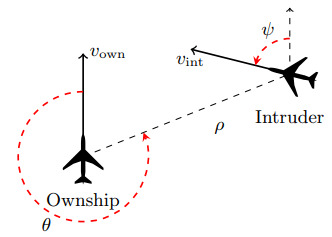
\includegraphics[width=0.7\linewidth]{Images/ACASXugeometry}
	\caption[ACAS Xu]{ACAS Xu geometry}
	\label{fig:acasxugeometry}
\end{figure}

\subsection{Experiment Methodology}
We consider a set of accurate inputs and construct perturbation scenarios. A perturbation scenario consists of 
\begin{enumerate}
	\item The output order
	\item Inputs perturbed
\end{enumerate}

\subsubsection{Random Attack}
Unlike \ac{APS} that had a concrete value as an output, in \ac{ACAS-Xu} and \ac{HCAS}, the output action depends on the scores. 
In a random attack, if the normal output was $strong$ $right$ the attacker's goal
is to change the output to $COC$.
This would lead to a crash since according to the new output decision, there is no intruder in the vicinity, and the unmanned vehicle should keep following its original path. 
This can be done by adding a constraint that ensures that the score of $COC$ is the least among all other outputs. 
The orderings of other outputs is of no concern to the attacker so long $COC$ has the least score. 

For each perturbation scenario, we evaluate our attack efficacy for different orderings, which means that if the correct decision based on the scores is $1$, then we perturb the inputs such that the output changes to $2$.
For this to happen the score for $2$ has to be the least of all other outputs. 

$Attack$ $1$ in Table ~\ref{hcas} is an example of a random attack where we set one of the outputs to be the least of all the outputs. 
The ordering of rest of outputs does not matter because the decision is selected based on the output with the least score. 
We test it by checking for attacks by perturbing $1$, $2$ and $3$ inputs at a time. 
From a practical scenario, a random attack is useful for an attacker because
they just have to state one constraint in this case, $value(2)$ $<$ $(all$ $other$ $values)$.

\subsubsection{Targeted Attack}

 
In a targeted attack, if the original output was $strong$ $right$, the goal of the attacker is to change the output to $strong$ $left$. 
The difference from a random attack is that the attacker wants the order of all the other inputs also to be in a specific order. 
This is to avoid potentially getting detected, since if the score for $strong$ $left$ is the lowest and the next higher score is for $strong$ $right$, this can trigger conflicts that are likely to be detected. 
Hence, the attacker sets constraints with a specific order such that $strong$ $left$ is followed by $weak$ $left$. 

Multiple different orders are tested for in Table ~\ref{hcas}, ~\ref{hcas2}, ~\ref{hcas3} and ~\ref{acasxu} for \ac{HCAS} and \ac{ACAS-Xu}. 

We conducted two types of targeted attacks:
\begin{enumerate}
\item Total ordering: In total ordering, there is a specific order decided by the attacker.
\item Partial ordering: In partial ordering, the order is set only for the first two outputs.  
\end{enumerate}



\iffalse

Consider a set of five inputs for which the output is weak left. 
The output weak left indicates that the \ac{DNN} returns 4. 
The network is trained in a way such that the least value signifies the output that should be taken next. 
The attacker's goal is to change the output in a way such that the minimum value changes from weak left to weak right. 
To model this, we first add a delta value to the inputs as in our previous evaluation. 
To do so, we add constraints that force the output to 5 instead of 4; the constraints look of the form "$05 < $(All other outputs)".
\fi


 
The attacker can conduct various targeted attacks using the critical inputs as shown in Table ~\ref{hcas}, ~\ref{hcas2}, ~\ref{hcas3} and ~\ref{acasxu} for \ac{HCAS} and \ac{ACAS-Xu}. 



\iffalse
\subsection{FDI random attack} 
Constructing random \ac{RFDIA} attacks is slightly less effort for the attacker as compared to targeted attacks; this is because the constraints in a targeted setting are much tighter. 
Building on the previous example, if we have 5 inputs that give us the result as output 4, we need to perturb the inputs such that the output changes to any of the other possibilities such as output 1, output 2, output 3 and output 5.

In this case, we try out multiple different combinations that allow us to find the perturbations as shown in Table ~\ref{hcas}, ~\ref{hcas2}, ~\ref{hcas3} and ~\ref{acasxu} for \ac{HCAS} and \ac{ACAS-Xu}.
\fi

\subsection{Result Analysis}
Some interesting observations were:
\begin{enumerate}
	\item We found attacks where perturbing a single input was enough to change the output decision.  
	\item In a complete ordering targeted attack scenario, we were unable to find a single successful attack. We believe this was so because the constraints were too tight. 
	\item When we tried finding the smallest perturbation, several experiments timed out but finding a perturbation between $delta$ was successful. 
\end{enumerate}	


\section{Summary}
\begin{enumerate}
	\item Overall, we conducted ~19,000 attacks for \ac{APS} out of which ~7200 attacks were successful, and took less than 1 second per attack. 
	\item We conducted ~30 \ac{HCAS} random attacks out of which ~20 were successful, and the maximum amount taken by the attacks was 41 seconds.
	\item We conducted ~7 targeted attacks for \ac{HCAS} out of which 1 attack was successful.
	\item We conducted ~140 \ac{ACAS-Xu} random attacks out of which ~32 were successful, and the maximum amount taken by the attacks was 7228 seconds.
	\item We conducted ~16 targeted attacks for \ac{HCAS}, out of which 2 attacks was successful.
\end{enumerate}

 
These results are shown in Table ~\ref{summary}.

Thus we can see that synthesizing \ac{RFDIA} attacks can be easily accomplished by the attacker in a small amount of time using \tool. 
We have also tried out multiple different combinations of attacks keeping multiple attacker scenarios in mind, and show that for systems such as \ac{APS} perturbing a single input out of the 74 inputs is enough to cause damage in Table ~\ref{APS}.
Similarly for \ac{HCAS} and \ac{ACAS-Xu}, we observe  from Table ~\ref{hcas}, ~\ref{hcas2}, ~\ref{hcas3} and ~\ref{acasxu} that perturbing a single input in certain scenarios is enough to cause output deviation. 

 \begin{table}[h!]
 	%\centering
 	\caption{Results Summary}
 	\label{summary}
 	\begin{tabular}{l|S|r|l}
 		\textbf{Inputs-pert} & \textbf{Total} &  \textbf{Successful} & \textbf{Mean-Time/ } \\
 		urbed/Attack &  Attacks &  Attacks &  Attack(s) \\
 		\hline
 		\multicolumn{4}{c}{APS}\\
 		\hline
 		1 &  518& 120 &  0.0015\\
 		2 &  18907& 7175 &  0.002\\
 		74 &  7& 7 &  0.03\\
 		\hline
 		\multicolumn{4}{c}{HCAS - Random}\\
 		\hline
 		%\textbf{HCAS}&  &   & \\
 		1 &  12& 5 &  3.87\\
 		2 &  12& 11 &  32.89\\
 		3 &  4&  4&  41.14\\
 		\hline
 		\multicolumn{4}{c}{HCAS - Targeted (Partial Ordering)}\\
 		\hline
 		%\textbf{HCAS}&  &   & \\
 		1 &  3& 1&  2.14\\
 		2 &  3& 0 &  2.91\\
 		3 &  1&  0&  2.74\\
 		\hline
 		\multicolumn{4}{c}{ACAS Xu - Random}\\
 		\hline
 		%\textbf{HCAS}&  &   & \\
 		1 &  20& 2&  100.11\\
 		2 &  40& 9& 548.72\\
 		3 &  40& 12&  1452.176\\
 		4 &  20&  8&  5029.58\\
 		5 &  20&  2&  7228.966\\
 		\hline
 		\multicolumn{4}{c}{ACAS Xu- Targeted (Partial Ordering)}\\ 
 		\hline
 		%\textbf{HCAS}&  &   & \\
 		1 &  5& 0&  297.2\\
 		2 &  10& 1 &  23595.58\\
 		5 &  1&  1&  8311.21\\
 		\hline
 		\hline
 	\end{tabular}
 \end{table}

\chapter{Discussion}
In this section we discuss how to model our insights into modeling robhust \karthik{Spell Check Fail!} 
DNNs by two approaches. \karthik{Did you mean leverage insights ? Also, what're the approaches for ?} 
We also discuss some limitations in our approach.

\section{Designing Robust DNNs}
From our experience in working with three different types of DNN based CPS to attack the systems, we realized that there are two ways to construct or build robust DNN based systems. 
\karthik{Can you say a little bit about how you came to this realization ? Was it based on the experimental results ?}

\section{Designing Robust DNN from scratch}
The biggest difference between APS and ACAS Xu apart from the DNN size was the robustness of the DNN. APS had a simple feed-forward architecture, where the network took the inputs, applied the non-linearity to the equations \karthik{non-linearity is not an action !},
 and calculated the outputs. Whereas ACAS Xu applied normalization to its inputs. \karthik{This is a phrase, not a sentence}

APS had accompanying DNNs that kept\karthik{Duh ?} did a range check to ensure that the output prediction lies within certain bounds \karthik{Did you mean specified bounds ?}. 
This was easier to break as per our attack model as compared to ACAS Xu\karthik{Can we quantify easier? Also, by break, I guess you mean attack?}. 
In ACAS Xu, due to the normalization of the inputs, the perturbations had to be carefully designed since one input perturbation did not easily perturb the outputs easily \karthik{Too many easilys!}. 
We can also observe the percentage of successful attacks from Table II \karthik{Symbolic ref.?} in APS and ACAS Xu. \karthik{What did you observed about them?}
Hence, we believe that applying techniques while training and modeling DNN architecture can significantly help prevent \attack. \karthik{This is a vacuous statement. What techniques are these ? How does one go about designing such a DNN?}

\section{Debugging existing DNN using \tool}
Given there exists a system with DNN similar to that of APS without inbuilt mechanisms, we believe that our tool can help in debugging the DNN by constructing a comprehensive list of cost functions and running the model for different scenarios. This might not provide complete coverage but can certainly help in the falsification process. 
\karthik{So what's falsification here. Also, it seems like an overly restrictive statement to make about the similarity with APR. What's inbuilt mechanism here ?}

\section{ Limitations}

There are 2 limitations in our work.
First, we are assuming that the attacker has access\karthik{Read or write ? Be specific !} to the weights and the bias. However, in a more ideal attack scenario \karthik{for the attacker ?}, if we \karthik{Who's we?} can find a way to  attack the system without knowing the weights and bias of the system, that would be really interesting \karthik{Please avoid weasel words like interesting - make it clear what is of interest}. %Figuring out FDI attacks in that scenario would be challenging yet rewarding. 
Second, for bigger systems such as ACAS Xu, we observed that running all combinations was taking a lot of time (approx 13 hours), only to tell us that no attack exists \karthik{I suppose us is we as the researcher here. Also, is the time taken a function of the attacks or the network ?}. We think there is scope of improvement to provide speedups by applying clever heuristics to the model. \karthik{Perhaps give 1-2 examples of heuristics here.}


%The limitation of our work is that we do not evaluate the completeness of our approach. We show experimentally that our technique always provides us a solution if the model is properly modeled and if there are attacks possible. Otherwise, it returns an infeasible model.  Since the modeling of the network is represented as a set of well-defined equations it is always going to return a solution if it exists. If no solution exists then it will return the model is infeasible. 
%The interesting part of our approach is that we are not trying to verify but instead we are trying to find feasible FDI attacks for the system. 
\label{section:limitations}
\include{futurework}
\chapter{Related Work}
\label{relatedwork}

We have classified related work into four broad categories. 
The first category discusses the verification techniques that have emerged to verify DNNs. We highlight why those techniques cannot directly be used for our application. The second discusses work done in the \ac{FDIA} community for classic control theory modeled systems, and why our work is required when \ac{DNN}s replace control theory equations. 
In the third category, we discuss multiple applications where DNNs have replaced or have been added to the CPS. This provides a glimpse into how the DNNs are being utilized in safety-critical applications. Furthermore, this motivates the need for a technique that can generalize to different settings of DNN based CPS.
 Finally, in the last category, we discuss adversarial attacks that have gained a lot of attention in the Machine Learning(ML) community and how are they different from our \attack. 
\section{Verification of CPS}
%Providing formal guarantees for CPS has always been an important part of the literature. The reason is due to their safety-critical nature. 

%\subsection{Control Theory CPS }
%\subsection{DNN based CPS}
Formally verifying DNN based CPS has recently gained a lot of momentum. Researchers have proposed automated verification mechanisms that use techniques involving SMT solvers, symbolic execution and MILP \cite{10.1007/978-3-642-14295-6_24}, \cite{article}, \cite{10.1007/978-3-319-63387-9_5}. 
However, the modeling that has been done for those interfaces cannot be directly used for our use case without significant modifications. 
The goal of these techniques is to conduct an input-output range analysis to establish bounds for the DNN for its correctness. Our work focuses not on conducting a bound analysis, but on finding the inputs for changing the outcome of a CPS under a constrained setting for a FDIA. Also, the approaches focus more on verifying certain properties such as reachability analysis that do not account for \attack.

Pulina et al.\cite{10.1007/978-3-642-14295-6_24} proposed one of the first approaches for verifying DNN safety properties using abstraction refinement. They further abstract \cite{article} the nonlinear activation functions in a linear arithmetic \ac{SMT} formula but their application and abstraction interface is different from ours. 
They then use a counterexample based approach for abstract refinement. There has been further work by Katz et al.\cite{10.1007/978-3-319-63387-9_5} in verifying the networks using SMT solvers where they build rules for handling the ReLU activation function. Most of work we have mentioned above in this domain utilizes the state-of-the art solvers Z3 and CVC4. However, all the existing techniques focus on proving robustness properties \cite{NIPS2016_6339} for DNNs that cannot detect or produce FDIA. Xiang at al.\cite{xiang2017output} focuses on an output reachable estimation for NN using simulation-based methods. There have been multiple methods proposed to conduct a reachability analysis for DNN using MILP/SMT approach \cite{10.1145/3302504.3313351} \cite{ehlers2017formal} \cite{10.1007/978-3-319-63387-9_5} \cite{lomuscio2017approach} \cite{article}. Ivanov et al. \cite{ivanov2018verisig} proposes a verification framework for verifying DNN based controllers by abstracting the problem into a hybrid system verification problem.  


\section{False Data Injection Attacks (FDIA) in traditional systems}
%FDI attacks in CPS in different domains. Difference in terms of modelling of systems. Sparse FDI attacks
Attacking a CPS by exploiting the deep integration of the physical-nature and cyber- nature of the systems has lead to the emergence of FDIAs. 
There are two main categories of FDI attacks that have been proposed in the literature: random FDIA and targeted FDIA. Random FDIA are generated by randomly changing the inputs to cause changes in the state estimation. Targeted FDIAs are the more interesting ones from an attackers perspective, because they have to synthesize the exact values of inputs to cause a change in the output without triggering alarms. Our work focuses on synthesizing both random and targeted FDIAs under a specific set of constraints based on the specification documentation that we explain in Chapter ~\ref{background}. 

In FDI attacks, the attacker's goal is to compromise the sensor inputs to mislead the state estimation process \cite{e3f0020abba24d4389aff937fe8bcdd5}. Liu et al. \cite{10.1145/1952982.1952995} introduced the class of FDIA for electric power grids to introduce arbitrary errors into certain state variables without being detected. Giannini et al. \cite{unknown} generate FDIA under a specific setting, 
where they introduce new information as constraints in the state estimator under the assumption that the new information is not available to the attacker. These techniques generate FDIA for systems modeled using control theory in order to cause a wrong state estimation without getting detected. Our work studies the CPS constructed using \ac{DNN}s. We demonstrate if  \ac{FDIA} would work in different constraint settings. 
Bobba et al. \cite{Bobba2010DetectingFD} show that by protecting a strategically selected set of sensor measurements, it is possible to detect the attacks proposed by Liu at al. \cite{10.1145/1952982.1952995}.
% Bai et al. \cite{bai2020aigan} proposes AI-GAN which provides a boost up over previous adversarial examples techniques. In contrast, our work is not focusing on adversarial examples for DNNs but FDIA for DNN based CPS in a constrained environment. 

\section{DNN controllers in CPS}
This line of work focuses on intelligent control using \ac{DNN} in designing the control systems. %As discussed in the Problem Formulation section NN allow the input-output mapping because of the nodes connecting in a network.
Fukuda et al. \cite{170966} show how NN can be utilized in industrial systems. Cong et al. \cite{Cong} proposes a recurrent neural network that is used to create a Proportional–Integral–Derivative (PID, K$_p$, K$_i$ and K$_d$)  neural network (PIDNN). 
This allows the network to converge more quickly since PIDNN has one hidden layer with 3 neurons that represent K$_p$, K$_i$ and K$_d$ that are used in traditional PID controllers. Wang et al. \cite{Wang2016ACA} proposes a double layer architecture for a non-linear system using adaptive NN control and Nonlinear Model Predictive Control (NMPC).

\section{Deep Neural Network Security}
%ML security such as adversarial ML
%adding noise to the inputs to change classification but they are based on RNN and other such networks- we use MILP optimization in order to find attacks that cause slight deviations and do not necessarily change the output
%DNNs are susceptible to attacks as is.

Adversarial machine learning emerged when Szegedy et al.  \cite{Szegedy2013IntriguingPO} showed that the input-output mappings for \ac{DNN}s are not continuous and it is possible to perturb the inputs by small amounts such that the classification changes. 
Since then there has been a lot of work exploring different types of adversarial attacks. Deng et al. \cite{deng2020analysis} analyzes five types of adversarial attacks in autonomous driving models. 
ConAML \cite{li2020conaml} explores constrained adversarial attacks for \ac{CPS} under different settings. They propose a best effort algorithm to iteratively generate adversarial examples but don't consider the physical notion of systems for their attack model. We, on the other hand, introduce \attack  that generate ripples based on constraints. 
Wang et al. \cite{217595} proposes ReLUVal that uses symbolic execution to show that the DNN based systems are free from security vulnerabilities to ensure that in specific intervals, the system is free from attacks; we use MILP that provides us the ability to model different cost functions for different attacks; symbolic execution does not contain this. 
\newline 
\newline 
%Summary
This chapter covers the various techniques that have been used in verification of DNNs, and explains why none of the existing techniques are suitable for our use case. 
We further introduce the various \ac{FDIA} conducted in classical control theory systems and their approaches for demonstrating the attacks. 
We then briefly describe the shift from control theory models to \ac{DNN} based models for \ac{CPS}.
Finally, we explain the security analysis explored in \ac{DNN}s. 
\chapter{Conclusion}
\label{conclusion}


We discuss two main approaches that can help researchers or developers design error-free \ac{DNN}s. 
We also discuss some limitations in our approach.
Finally, we conclude and discuss some future work.


\section{Designing Robust DNNs}
From our experience in attacking three different types of \ac{DNN} based CPS we realized that there are two ways to construct or build robust \ac{DNN} based systems. 
The two things that help us in building our intuition were:
\begin{enumerate}
	\item Building and running the models on \ac{MILP} solvers helped us understand the power in terms of reasoning about \ac{DNN} based systems for observing non-obvious security properties such as ripples. 
	\item Attacking three practical systems helped  us come to a realization how to design robust \ac{DNN}  by adding layers of complexity to \ac{DNN}. 
\end{enumerate}


\subsection{Effects of normalization and attacks}
The biggest difference between \ac{APS} and \ac{ACAS-Xu} apart from the \ac{DNN} size was the robustness of the \ac{DNN}. 
\ac{APS} has a fully-connected feed-forward architecture, where the network takes the inputs and passes them through the hidden layers to compute the output. 
\ac{ACAS-Xu} is also a fully-connected \ac{DNN} however, it includes normalization.
This means that we have to try out more combinations of input variable perturbations to find if an attack exists. 
Small perturbations during the \ac{FDIA} get masked due to the normalization layer; changing an input value from $5$ to $10$ has little to no effect on the \ac{DNN} if the normalization layer normalizes a range of inputs to a value between $0$ and $1$. 
Thus we have to perturb by values large enough to induce a change in the normalized representation. 
We also observed that in many cases, despite large enough perturbation we were unable to generate \ac{RFDIA} in \ac{HCAS} and \ac{ACAS-Xu} as shown in Chapter ~\ref{evaluation}.
Intuitively due to the nature of the attacks based on the sizes of \ac{APS} and \ac{ACAS-Xu} we should have been able to generate significantly more \ac{RFDIA}; instead we observe that despite the bigger search space in \ac{HCAS} and \ac{ACAS-Xu} we found very few \ac{RFDIA} as compared to \ac{APS}. 


We believe that normalization makes it difficult for attacker to compromise the system. 
It does not eliminate the possibility of conducting attacks entirely, but makes the system somewhat more secure. 

\subsection{Effects of DNN size and attacks}
The \ac{APS} was a relatively smaller system compared to \ac{ACAS-Xu} and \ac{HCAS}.
We observe that due to the smaller and much less complex nature of \ac{APS}, we are able to try out more combinations and hence are able to find more attacks. 
Every attack in \ac{APS} takes less than a minute to generate if it exists or tell us if it does not; \ac{HCAS} and \ac{ACAS-Xu} on the other hand can take hours just to tell us that there is no attack. 
This restricts and allows us to conduct a limited number of combinations to find attacks. 
Hence, comparing between small systems such as \ac{APS}, and relatively bigger systems, such as \ac{HCAS} and \ac{ACAS-Xu}, we observe that the small system size enables us to generate more attacks and cover more combinations. 
When we compare \ac{HCAS} and \ac{ACAS-Xu} we observe a similar behavior; \ac{HCAS} took less time per attack and hence we were able to explore more space and find successful instances of attacks. 
The reason we consider time an important factor is because if it takes 100 days to find an attack, attacks become more expensive to find. 
Hence, our focus is not to generate the attack in seconds but our goal is to come to a reasonable trade-off between time and size to generate attacks. 

Thus, based on our observations we can say that designing bigger systems can help make systems more secure but this is true given they are well trained since if a network is poorly trained no matter how big it is will not help secure it. 




\subsection{Summary}
Thus keeping the above two principles in mind, adding normalization and having certain level of complexity in the \ac{DNN} can significantly help the \ac{DNN}s be more secure. 
This will obviously not work in every situation because the \ac{DNN} might have other flaws but it is good to keep this in mind when designing networks especially for safety-critical systems. 

\section{Debugging existing DNN using \tool}
In our work we used \tool to generate attacks for trained \ac{DNN}s that also tell us if in a particular setting an attack does not exist. 
However, instead of trying to find attacks in the \ac{DNN} we can also use \tool in a slightly different way which is for debugging; it means that we can conduct an input-output pair generation to study if there are some abnormal pairs that are being generated. 
This can be seen as trying to generate the datasets from a trained model that can be used to understand the corner cases; cases can help the designers or researchers to understand how to modify the training data such that they can improve a \ac{DNN} performance by adding or removing from the datasets. 







\section{ Limitations  and Future Work}

There are 2 limitations that pave way for future work. 
\begin{enumerate}
	\item First, we are assuming that the attacker has read access to the weights and the bias of a \ac{DNN}.
	However, in an ideal scenario it is difficult to obtain read access to weights and bias of safety-critical systems such as \ac{CA} systems since they protect their systems by security by obscurity for an attacker. 
	Therefore, the attacker might need tools or techniques that allows them to attack the system without having knowledge about the internals of the network; also called as a black-box approach. 
	This would mean that with a short amount (preferably a couple of hours) the attacker is able to attack a black box system and conduct \ac{RFDIA} or other attacks. 
	\item Second, we observed that in complex \ac{DNN}s of our three systems, there were many cases when  \ac{ACAS-Xu} timed out and did not return us any results. 
	The time out occurred because the search space for the appropriate input-output pair was very huge. 
	However, we believe adding more precise bounds and limiting the search space can significantly scale our approach. 
	There is a possibility of designing clever heuristics for domain specific systems such as removing non required layers, pruning the \ac{DNN} appropriately, using algorithmic approaches to decrease time complexity of \ac{MILP} solvers. 
	
	\label{section:limitations}
	
\end{enumerate}




Finally, we believe that there are many more extensions that can be done with \tool. 
\begin{enumerate}
	\item First, it can be extended for multiple different application domains to find attacks.
	For instance \ac{AV} have multiple stacks of \ac{DNN}s to compute the output and \tool can be utilized to find attacks in multiple \ac{DNN}s.
	\item Second, one can try and model cost functions for an attack model different from ours and use our insights to generate attacks.
	This is because the modeling of the \ac{DNN} and \tool can be easily reused by integrating with different attack specific cost functions. 
\end{enumerate}


\section{Conclusion}
We demonstrate \tool, which is based on generating \attack using backend \ac{MILP} solvers. 

We address the two main challenges in synthesizing \attack: 
\begin{enumerate}
	\item Locating the critical inputs: 
	
	\item finding the smallest perturbations for critical inputs to conduct \attack.
	
\end{enumerate}
To locate the critical inputs, we model a cost function and add $delta$ variable to the inputs and minimize the $delta$. 
This tells the attacker changing the minimal set of inputs by smallest possible amounts will result in wrong output predictions.

Based on our experiments, we conclude that:

\begin{enumerate}
	\item The first observation is that it is easier (in terms of time) to find attacks on small-sized DNN based CPS. 
	APS took less than a second for finding an attack whereas ACAS Xu took as high as 5 hours and timed out for certain constraints. 
	
	\item We found fewer attacks in ACAS Xu as compared to APS indicating  that ACAS Xu is a more robustly designed network due to the existence of normalization that makes it difficult to generate ripples. 
	Hence, it is possible to design robust \ac{DNN} while designing the architectures by integrating such features. 
	
	\item Finally, we observe that the choice of the cost function and the intervals affects the state explosion of the system. 
	If there is a minimization function on the input perturbations, it takes much longer to compute and can also lead to state-space in certain cases as comparing with other function. 
\end{enumerate}




\iffalse
We have addressed security as an optimization problem by modeling the Deep Neural Network as a Mixed Integer Linear model. This is the first step to automatically synthesize attacks called ripple attacks that on small perturbations to the input propagate further to cause output perturbations. 

We discussed the modeling details, designing attack specific cost functions \smi{change 'cost functions' to 'target inputs/perturbation bounds'; cost functions mean objective function which doesn't change for us}, finding critical inputs and finally finding the minimum perturbations for a successful attack that we call as a ripple attack. We show our evaluation on three systems of different sizes. Our biggest system size is (5,50,50,50,50,50,5). We model the cost functions such that even for big systems, our approach does not blow up \smi{we should chat and clarify the meaning of cost functions in this context}. We chose the three systems that are practical safety-critical systems that is an artificial pancreas system, and two aircraft collision avoidance networks.

For the medical system which is a considerably smaller system than our collision avoidance system, we are able to find the critical inputs and synthesize minimum perturbations in less than a second. For bigger system with more layers and number of neurons per layer, we are successfully able to synthesize attacks within a minute. 

We believe that using our technique to find similar attacks in systems such as self-driving cars that have multiple DNNs instead of one in their control system would be an interesting future work. As mentioned in the discussion section using our approach for tracing error propagation is another interesting use case. Finally, modeling application specific heuristics for systems such as surgical arm to synthesize attacks is another interesting topic for future research. 
\fi 
%\chapter{Discussion}
In this section we discuss how to model our insights into modeling robhust \karthik{Spell Check Fail!} 
DNNs by two approaches. \karthik{Did you mean leverage insights ? Also, what're the approaches for ?} 
We also discuss some limitations in our approach.

\section{Designing Robust DNNs}
From our experience in working with three different types of DNN based CPS to attack the systems, we realized that there are two ways to construct or build robust DNN based systems. 
\karthik{Can you say a little bit about how you came to this realization ? Was it based on the experimental results ?}

\section{Designing Robust DNN from scratch}
The biggest difference between APS and ACAS Xu apart from the DNN size was the robustness of the DNN. APS had a simple feed-forward architecture, where the network took the inputs, applied the non-linearity to the equations \karthik{non-linearity is not an action !},
 and calculated the outputs. Whereas ACAS Xu applied normalization to its inputs. \karthik{This is a phrase, not a sentence}

APS had accompanying DNNs that kept\karthik{Duh ?} did a range check to ensure that the output prediction lies within certain bounds \karthik{Did you mean specified bounds ?}. 
This was easier to break as per our attack model as compared to ACAS Xu\karthik{Can we quantify easier? Also, by break, I guess you mean attack?}. 
In ACAS Xu, due to the normalization of the inputs, the perturbations had to be carefully designed since one input perturbation did not easily perturb the outputs easily \karthik{Too many easilys!}. 
We can also observe the percentage of successful attacks from Table II \karthik{Symbolic ref.?} in APS and ACAS Xu. \karthik{What did you observed about them?}
Hence, we believe that applying techniques while training and modeling DNN architecture can significantly help prevent \attack. \karthik{This is a vacuous statement. What techniques are these ? How does one go about designing such a DNN?}

\section{Debugging existing DNN using \tool}
Given there exists a system with DNN similar to that of APS without inbuilt mechanisms, we believe that our tool can help in debugging the DNN by constructing a comprehensive list of cost functions and running the model for different scenarios. This might not provide complete coverage but can certainly help in the falsification process. 
\karthik{So what's falsification here. Also, it seems like an overly restrictive statement to make about the similarity with APR. What's inbuilt mechanism here ?}

\section{ Limitations}

There are 2 limitations in our work.
First, we are assuming that the attacker has access\karthik{Read or write ? Be specific !} to the weights and the bias. However, in a more ideal attack scenario \karthik{for the attacker ?}, if we \karthik{Who's we?} can find a way to  attack the system without knowing the weights and bias of the system, that would be really interesting \karthik{Please avoid weasel words like interesting - make it clear what is of interest}. %Figuring out FDI attacks in that scenario would be challenging yet rewarding. 
Second, for bigger systems such as ACAS Xu, we observed that running all combinations was taking a lot of time (approx 13 hours), only to tell us that no attack exists \karthik{I suppose us is we as the researcher here. Also, is the time taken a function of the attacks or the network ?}. We think there is scope of improvement to provide speedups by applying clever heuristics to the model. \karthik{Perhaps give 1-2 examples of heuristics here.}


%The limitation of our work is that we do not evaluate the completeness of our approach. We show experimentally that our technique always provides us a solution if the model is properly modeled and if there are attacks possible. Otherwise, it returns an infeasible model.  Since the modeling of the network is represented as a set of well-defined equations it is always going to return a solution if it exists. If no solution exists then it will return the model is infeasible. 
%The interesting part of our approach is that we are not trying to verify but instead we are trying to find feasible FDI attacks for the system. 
\label{section:limitations}
%    2. Main body
% Generally recommended to put each chapter into a separate file
%\chapter{Related Work}
\label{ch:Chapter2}



We have classified related work into four broad categories. The first category discusses the verification techniques that have emerged to verify DNNs. We highlight why those techniques cannot directly be used for our application. The second discusses work done in the FDIA community for classic control theory modeled systems and why our work is required to understand the consequences of deploying DNNs in CPS.  In the third category, we discuss multiple applications where DNNs have replaced the traditional CPS. This provides a glimpse into how the DNNs are being utilized in safety-critical applications. Furthermore, this motivates the need for a technique that can generalize to different settings of DNN based CPS. Finally, in the last category we discuss the adversarial attacks that have gained a lot of attention in the Machine Learning community and how are they different from our \attack. 
\subsection{Verification of CPS}
%Providing formal guarantees for CPS has always been an important part of the literature. The reason is due to their safety-critical nature. 

%\subsection{Control Theory CPS }
%\subsection{DNN based CPS}
Formally verifying DNN based CPS has recently gained a lot of momentum. Researchers have proposed automated verification mechanisms that use techniques involving SMT solvers, symbolic execution and MILP. However, the modeling that has been done for those interfaces cannot be directly used for our use case without modifications. The goal of these techniques is to conduct an input-output range analysis to establish bounds for the DNN. Our work focuses not on conducting a bound analysis but finding the optimal inputs for changing the outcome of a CPS under a constrained setting for a FDIA. Also, the approaches focus more on verifying certain properties such as reachability analysis that do not account for \attack.

Pulina et al.\cite{10.1007/978-3-642-14295-6_24} proposed one of the first approaches for verifying DNN safety properties using abstraction refinement. They further abstract \cite{article} the nonlinear activation functions in a linear arithmetic SMT formula. They then use counterexample based approach for abstract refinement. There has been further work by Katz et al.\cite{10.1007/978-3-319-63387-9_5} in verifying the networks using SMT solvers where they build rules for handling the ReLU activation function. Most of work we have mentioned above in this domain utilizes the state-of-the art solvers Z3 and CVC4. However, all the existing techniques focus on proving robustness properties \cite{NIPS2016_6339} for DNNs that cannot detect or produce FDIA. Xiang at al.\cite{xiang2017output} focuses on an output reachable estimation for NN using simulation-based methods. There have been multiple methods proposed to conduct a rechability analysis for DNN using MILP/SMT approach \cite{10.1145/3302504.3313351} \cite{ehlers2017formal} \cite{10.1007/978-3-319-63387-9_5} \cite{lomuscio2017approach} \cite{article}. Ivanov et al. \cite{ivanov2018verisig} proposes a verification framework for verifying DNN based controllers by abstracting the problem into a hybrid system verification problem.  
%\subsection*{Cyber-Physical Systems Security}
%Sensor spoofing attacks- multiple types such as gps spoofing, most common ones demonstrated are FDI.

\subsection{False Data Injection Attacks (FDIA) in traditional systems}
%FDI attacks in CPS in different domains. Difference in terms of modelling of systems. Sparse FDI attacks
Attacking the CPS by exploiting the deep integration of the physical-nature and cyber nature of the systems has lead to the emergence of FDIAs. 
There are two main categories of FDI attacks that have been proposed in the literature: random FDIA and targeted FDIA. Random FDIA are generated by randomly changing the inputs to cause changes in the state estimation. Targeted FDIAs are the more interesting ones from an attackers perspective because in this case, they have to synthesize the exact values of inputs to cause a change in the output without triggering alarms. Our work focuses on synthesizing random and targeted FDIAs under specific set of constraints based on the specification documentation. 

In FDI attacks, the attacker's goal is to compromise the sensor inputs to mislead the state estimation process \cite{e3f0020abba24d4389aff937fe8bcdd5}. Liu et al. \cite{10.1145/1952982.1952995} introduced the class of FDIA for electric power grids to introduce arbitrary errors into certain state variables without being detected. Giannini et al. \cite{unknown} generate FDIA under specific setting %\karthik{What does this mean?}
where they introduce new information as constraints in the state estimator under the assumption that the new information is not available to the attacker. This can basically be seen as security by obscurity. These techniques generate FDIA for systems modeled using control theory in order to cause a wrong state estimation without getting detected. Our work looks at the CPS constructed using \ac{DNN}. We try to understand if \ac{FDIA} would work in different constraint setting. Bobba et al. \cite{Bobba2010DetectingFD} show that by protecting a strategically selected set of sensor measurements it is possible to detect the attacks proposed by Liu at al. \cite{10.1145/1952982.1952995}.
% Bai et al. \cite{bai2020aigan} proposes AI-GAN which provides a boost up over previous adversarial examples techniques. In contrast, our work is not focusing on adversarial examples for DNNs but FDIA for DNN based CPS in a constrained environment. 

\subsection{DNN controllers in CPS}
This section focuses on intelligent control primarily due to the introduction of neural networks(NN) in designing the control systems. This subsection discusses how different types of \ac{DNN} are utilized in \ac{CPS} modeling. There are multiple types of \ac{DNN} architectures that have been proposed by \ac{CPS} designers in the recent years. This work is mentioned to provide an intuition of the different models that exist and how none of them have a common means of abstraction or representation.   %As discussed in the Problem Formulation section NN allow the input-output mapping because of the nodes connecting in a network.


Fukuda et al. \cite{170966} show how NN can be utilized in multiple industrial systems. Cong et al. \cite{Cong} proposes a recurrent neural network that is used to create a PID neural network (PIDNN). A proportional–integral–derivative controller is a control loop mechanism employing feedback that is widely used in industrial control systems and a variety of other applications requiring continuously modulated control. This allows the network to converge faster since PIDNN has one hidden layer with 3 neurons that represent K$_p$, K$_i$ and K$_d$ that are used in traditional PID controllers. Wang et al. \cite{Wang2016ACA} proposes a double layer architecture for a non-linear system using adaptive NN control and Nonlinear Model Predictive Control (NMPC). However, none of the mentioned work explores the security affects of replacing the standard controllers with DNNs. Our work specifically looks into understanding the affects of replacing the standard controllers with DNNs and \attack is one of the results.

\subsection{Deep Neural Network Security}
%ML security such as adversarial ML
%adding noise to the inputs to change classification but they are based on RNN and other such networks- we use MILP optimization in order to find attacks that cause slight deviations and do not necessarily change the output
%DNNs are susceptible to attacks as is.

The deep learning security comprises the adversarial examples field which was introduced by Szegedy et al. \cite{Szegedy2013IntriguingPO} where they showed that the input-output mappings for the DNNs are not continuous and it is possible to perturb the inputs by small amounts such that the classification changes. Since then there has been a lot of work exploring different types of adversarial attacks. There are two ways of attacking the \ac{ML} models: data poisoning \cite{DBLP:journals/corr/abs-1903-01666}, and adversarial attacks broadly survey by Papernot et al. \cite{DBLP:journals/corr/PapernotMSW16}. Data poisoning attacks perturb the data during the training phase of the networks whereas adversarial attacks usually act on a trained network by falling the specific input set that creates erroneous perturbations in the output. 



 Deng et al. \cite{deng2020analysis} analyses five types of adversarial attacks in autonomous driving models.  ConAML \cite{li2020conaml} explores the constrained adversarial attacks for cyber-physical systems under different settings. They propose a best effort algorithm to iteratively generate adversarial examples. We on the other hand introduce \attack  that generate ripples based on constraints. We are not trying to find inputs that cause erroneous perturbations due to the deviations but due to the design of the systems. 
  Wang et al. \cite{217595} proposes ReLUVal that uses symbolic execution to show that the DNN based systems are free from security vulnerabilities. They use symbolic execution to ensure that in specific intervals the system is free from attacks whereas we formalize the \ac{CPS} using \ac{MILP} . 

%The goal of our work is to find if a DNN based CPS has ripples and to do so we use MILP whose goal is to find a \attack if it exists.
% \karthik{What about the ReLuVal paper [37] ?}

%\aarti{Add more papers here}
%CPS verification 
%\include{model}
%\include{impl}
%\chapter{Discussion}
In this section we discuss how to model our insights into modeling robhust \karthik{Spell Check Fail!} 
DNNs by two approaches. \karthik{Did you mean leverage insights ? Also, what're the approaches for ?} 
We also discuss some limitations in our approach.

\section{Designing Robust DNNs}
From our experience in working with three different types of DNN based CPS to attack the systems, we realized that there are two ways to construct or build robust DNN based systems. 
\karthik{Can you say a little bit about how you came to this realization ? Was it based on the experimental results ?}

\section{Designing Robust DNN from scratch}
The biggest difference between APS and ACAS Xu apart from the DNN size was the robustness of the DNN. APS had a simple feed-forward architecture, where the network took the inputs, applied the non-linearity to the equations \karthik{non-linearity is not an action !},
 and calculated the outputs. Whereas ACAS Xu applied normalization to its inputs. \karthik{This is a phrase, not a sentence}

APS had accompanying DNNs that kept\karthik{Duh ?} did a range check to ensure that the output prediction lies within certain bounds \karthik{Did you mean specified bounds ?}. 
This was easier to break as per our attack model as compared to ACAS Xu\karthik{Can we quantify easier? Also, by break, I guess you mean attack?}. 
In ACAS Xu, due to the normalization of the inputs, the perturbations had to be carefully designed since one input perturbation did not easily perturb the outputs easily \karthik{Too many easilys!}. 
We can also observe the percentage of successful attacks from Table II \karthik{Symbolic ref.?} in APS and ACAS Xu. \karthik{What did you observed about them?}
Hence, we believe that applying techniques while training and modeling DNN architecture can significantly help prevent \attack. \karthik{This is a vacuous statement. What techniques are these ? How does one go about designing such a DNN?}

\section{Debugging existing DNN using \tool}
Given there exists a system with DNN similar to that of APS without inbuilt mechanisms, we believe that our tool can help in debugging the DNN by constructing a comprehensive list of cost functions and running the model for different scenarios. This might not provide complete coverage but can certainly help in the falsification process. 
\karthik{So what's falsification here. Also, it seems like an overly restrictive statement to make about the similarity with APR. What's inbuilt mechanism here ?}

\section{ Limitations}

There are 2 limitations in our work.
First, we are assuming that the attacker has access\karthik{Read or write ? Be specific !} to the weights and the bias. However, in a more ideal attack scenario \karthik{for the attacker ?}, if we \karthik{Who's we?} can find a way to  attack the system without knowing the weights and bias of the system, that would be really interesting \karthik{Please avoid weasel words like interesting - make it clear what is of interest}. %Figuring out FDI attacks in that scenario would be challenging yet rewarding. 
Second, for bigger systems such as ACAS Xu, we observed that running all combinations was taking a lot of time (approx 13 hours), only to tell us that no attack exists \karthik{I suppose us is we as the researcher here. Also, is the time taken a function of the attacks or the network ?}. We think there is scope of improvement to provide speedups by applying clever heuristics to the model. \karthik{Perhaps give 1-2 examples of heuristics here.}


%The limitation of our work is that we do not evaluate the completeness of our approach. We show experimentally that our technique always provides us a solution if the model is properly modeled and if there are attacks possible. Otherwise, it returns an infeasible model.  Since the modeling of the network is represented as a set of well-defined equations it is always going to return a solution if it exists. If no solution exists then it will return the model is infeasible. 
%The interesting part of our approach is that we are not trying to verify but instead we are trying to find feasible FDI attacks for the system. 
\label{section:limitations}
%\include{conclusions}

%    3. Notes
%    4. Footnotes

%    5. Bibliography
\begin{singlespace}
\raggedright
	\bibliography{bib}
\bibliographystyle{ieeetr}
\end{singlespace}

\appendix
%    6. Appendices (including copies of all required UBC Research
%       Ethics Board's Certificates of Approval)
%\include{reb-coa}	% pdfpages is useful here

%\include{appendix}

\backmatter
%    7. Index
% See the makeindex package: the following page provides a quick overview
% <http://www.image.ufl.edu/help/latex/latex_indexes.shtml>


\end{document}
